\documentclass[12pt,a4paper]{article}

% ─── Pakete ──────────────────────────────────────────────────────────────────
\usepackage[T1]{fontenc}
\usepackage[utf8]{inputenc}

\usepackage{geometry}
\geometry{a4paper, margin=2.5cm}

\usepackage{amsmath,amssymb,amsthm}
\usepackage{mathtools}
\usepackage{bm}
\usepackage{graphicx}
\usepackage{xcolor}
\usepackage{booktabs}
\usepackage{multirow}
\usepackage{array}
\usepackage{caption}
\usepackage{subcaption}
\usepackage{tikz}
\usetikzlibrary{arrows.meta,shapes.geometric,positioning,fit,
                backgrounds,matrix,calc,decorations.pathreplacing,
                shadows.blur,fadings}
\usepackage{pgfplots}
\pgfplotsset{compat=1.18}
\usepackage{algorithm}
\usepackage{algpseudocode}
\usepackage{listings}
\usepackage{enumitem}
\usepackage{hyperref}
\usepackage{cleveref}
\usepackage{natbib}
\usepackage{abstract}
\usepackage{titlesec}
\usepackage{fancyhdr}
\usepackage{lipsum}
\usepackage{microtype}
\usepackage{tcolorbox}
\tcbuselibrary{skins,breakable}

\setlist[itemize,1]{label=--}

% ─── Deutsche Bezeichner ─────────────────────────────────────────────────────
\renewcommand{\figurename}{Abbildung}
\renewcommand{\tablename}{Tabelle}
\renewcommand{\listfigurename}{Abbildungsverzeichnis}
\renewcommand{\listtablename}{Tabellenverzeichnis}
\renewcommand{\contentsname}{Inhaltsverzeichnis}
\renewcommand{\refname}{Literaturverzeichnis}
\renewcommand{\bibname}{Literaturverzeichnis}
\renewcommand{\abstractname}{Zusammenfassung}
\renewcommand{\appendixname}{Anhang}
\renewcommand{\proofname}{Beweis}
% algorithm-Paket: Algorithmus-Bezeichner
\floatname{algorithm}{Algorithmus}
\renewcommand{\listalgorithmname}{Algorithmenverzeichnis}
% cleveref: deutsche Bezeichner
\crefname{figure}{Abbildung}{Abbildungen}
\Crefname{figure}{Abbildung}{Abbildungen}
\crefname{table}{Tabelle}{Tabellen}
\Crefname{table}{Tabelle}{Tabellen}
\crefname{algorithm}{Algorithmus}{Algorithmen}
\Crefname{algorithm}{Algorithmus}{Algorithmen}
\crefname{equation}{Gleichung}{Gleichungen}
\Crefname{equation}{Gleichung}{Gleichungen}
\crefname{section}{Abschnitt}{Abschnitte}
\Crefname{section}{Abschnitt}{Abschnitte}
\crefname{subsection}{Abschnitt}{Abschnitte}
\Crefname{subsection}{Abschnitt}{Abschnitte}
\crefname{theorem}{Theorem}{Theoreme}
\Crefname{theorem}{Theorem}{Theoreme}
\crefname{lemma}{Lemma}{Lemmata}
\Crefname{lemma}{Lemma}{Lemmata}
\crefname{definition}{Definition}{Definitionen}
\Crefname{definition}{Definition}{Definitionen}
\crefname{corollary}{Korollar}{Korollare}
\Crefname{corollary}{Korollar}{Korollare}
\crefname{proposition}{Proposition}{Propositionen}
\Crefname{proposition}{Proposition}{Propositionen}
\crefname{remark}{Bemerkung}{Bemerkungen}
\Crefname{remark}{Bemerkung}{Bemerkungen}

% ─── Farben ──────────────────────────────────────────────────────────────────
\definecolor{nvidiaGreen}{RGB}{118,185,0}
\definecolor{nvidiaDark}{RGB}{29,29,29}
\definecolor{accentBlue}{RGB}{0,114,198}
\definecolor{accentCyan}{RGB}{0,188,212}
\definecolor{lightGray}{RGB}{245,245,245}
\definecolor{midGray}{RGB}{120,120,120}
\definecolor{deepPurple}{RGB}{74,20,140}

% ─── Theorem-Umgebungen ──────────────────────────────────────────────────────
\newtheorem{theorem}{Theorem}[section]
\newtheorem{lemma}[theorem]{Lemma}
\newtheorem{proposition}[theorem]{Proposition}
\newtheorem{corollary}[theorem]{Korollar}
\newtheorem{definition}[theorem]{Definition}
\newtheorem{remark}[theorem]{Bemerkung}
\newtheorem{example}[theorem]{Beispiel}

% ─── Section-Formatierung ────────────────────────────────────────────────────
\titleformat{\section}{\large\bfseries\color{nvidiaDark}}{{\color{nvidiaGreen}\thesection}}{0.5em}{}[\vspace{-2pt}\textcolor{nvidiaGreen}{\hrule height 0.8pt}\vspace{2pt}]
\titleformat{\subsection}{\normalsize\bfseries\color{nvidiaDark}}{\thesubsection}{0.5em}{}
\titleformat{\subsubsection}{\small\bfseries\itshape\color{accentBlue}}{\thesubsubsection}{0.5em}{}

% ─── Header/Footer ───────────────────────────────────────────────────────────
\pagestyle{fancy}
\fancyhf{}
\fancyhead[L]{\small\textcolor{midGray}{\textsc{Epp} \,|\, Skalierbare KI-Datenspeicherung}}
\fancyhead[R]{\small\textcolor{nvidiaGreen}{\textbf{NVIDIA GTC 2026}}}
\fancyfoot[C]{\small\textcolor{midGray}{\thepage}}
\renewcommand{\headrulewidth}{0.4pt}
\renewcommand{\headrule}{\hbox to\headwidth{\color{nvidiaGreen}\leaders\hrule height \headrulewidth\hfill}}

% ─── Listings ────────────────────────────────────────────────────────────────
\lstset{
  basicstyle=\ttfamily\scriptsize,
  keywordstyle=\color{accentBlue}\bfseries,
  commentstyle=\color{midGray}\itshape,
  stringstyle=\color{nvidiaGreen},
  numbers=left,
  numberstyle=\tiny\color{midGray},
  breaklines=true,
  frame=single,
  rulecolor=\color{lightGray},
  backgroundcolor=\color{lightGray}
}

% ─── Tcolorbox-Styles ────────────────────────────────────────────────────────
\tcbset{
  mybox/.style={
    enhanced, breakable,
    colback=lightGray, colframe=nvidiaGreen,
    fonttitle=\bfseries\small,
    boxrule=0.8pt, arc=3pt,
    left=4pt, right=4pt, top=4pt, bottom=4pt
  },
  keybox/.style={
    enhanced,
    colback=nvidiaDark!5, colframe=accentBlue,
    fonttitle=\bfseries\small\color{accentBlue},
    boxrule=1pt, arc=4pt,
    left=5pt, right=5pt, top=5pt, bottom=5pt
  }
}

% ─── Metadaten ───────────────────────────────────────────────────────────────
\hypersetup{
  pdftitle={Skalierbare Vektorisierung und KI-gestützte Strukturierung
            heterogener Großdaten: Ein Framework für On-Demand-Darstellung},
  pdfauthor={Stephan Epp},
  colorlinks=true,
  linkcolor=accentBlue,
  citecolor=nvidiaGreen,
  urlcolor=accentCyan
}

% ─────────────────────────────────────────────────────────────────────────────
\begin{document}

% ─── Titelbereich ────────────────────────────────────────────────────────────
\begin{center}
  \vspace*{0.2cm}
  {\small\textcolor{nvidiaGreen}{\textbf{NVIDIA GTC 2026 — Pregame Session}} \,·\,
   LinkedIn Tech Talk, 16\,Uhr, 16.\,März 2026}\\[0.5em]

  {\LARGE\bfseries\color{nvidiaDark}
   Skalierbare Vektorisierung und \\KI-gestützte Strukturierung von Großdaten}\\[0.3em]
  {\Large\bfseries\color{accentBlue}
   Ein Framework für On-Demand-Darstellung und\\[0.1em]
   dynamische Datenmorphologie}\\[0.7em]

  {\normalsize\bfseries Stephan Epp}\\[0.4em]
  {\small\textit{16. März 2026}}\\[0.8em]

  \begin{minipage}{0.88\linewidth}
    \begin{tcolorbox}[mybox, title={Abstract}]
      \small
      Die rasante Zunahme multimodaler Datenmengen — Videos, Bilder, Texte, 
      Audiodaten, Sensordaten — stellt fundamentale Herausforderungen an 
      Speicherarchitekturen und KI-gestützte Verarbeitungspipelines.
      Wir präsentieren \textbf{VADIS} (\textit{Vector-Adaptive Dynamic 
      Information Structure}), ein neuartiges Framework, das heterogene 
      Großdaten durch hierarchische Vektorisierung in einem universellen 
      semantischen Einbettungsraum $\mathcal{E} \subset \mathbb{R}^d$ 
      repräsentiert. VADIS ermöglicht es KI-Systemen, auf Anfragebedarf 
      (\textit{on demand}) beliebige Datenstrukturen effizient zu bilden, 
      zusammenzuführen und darzustellen. Kernbeiträge sind: (1) ein 
      modalitätsübergreifendes Einbettungsschema mit sublinearem 
      Speicherwachstum $O(n^{1-\epsilon})$, (2) ein hierarchischer 
      Indexierungsmechanismus (HVI) mit Anfrage-Komplexität 
      $O(\log^2 n)$, (3) ein On-Demand-Rendering-Protokoll (ODRP) für 
      die dynamische Strukturkomposition, sowie (4) eine NVIDIA-GPU-basierte 
      Parallelisierungsarchitektur, die lineare Skalierbarkeit bis zu 
      $10^{12}$ Datenpunkten demonstriert. Experimentelle Ergebnisse auf 
      dem LAION-5B-Datensatz und einem proprietären Video-Corpus 
      bestätigen überlegene Effizienz gegenüber aktuellen Baseline-Systemen.
    \end{tcolorbox}
  \end{minipage}\\[0.9em]
\end{center}

\tableofcontents
\newpage

% ─────────────────────────────────────────────────────────────────────────────
\section{Einleitung}
\label{sec:einleitung}
% ─────────────────────────────────────────────────────────────────────────────

Das digitale Universum expandiert mit exponentieller Geschwindigkeit. 
Schätzungen zufolge werden bis 2027 täglich über 120\,Zettabytes an 
neuen Daten generiert~\cite{idc2024}, wobei ein wachsender Anteil 
\emph{multimodal} ist — d.\,h., Video, Bild, Text und Sensordaten 
treten in engem semantischen Kontext auf. Gleichzeitig wächst die 
Anforderung an KI-Systeme, diese Daten nicht nur passiv zu speichern, 
sondern \emph{dynamisch} und \emph{strukturadaptiv} zu verarbeiten: 
Auf eine Nutzeranfrage hin soll das System in Echtzeit die optimale 
Datenstruktur \emph{konstruieren} und \emph{rendern}.

Aktuelle Systeme scheitern an dieser Anforderung aus drei Gründen:

\begin{enumerate}[leftmargin=1.2em, itemsep=0pt, topsep=2pt]
  \item \textbf{Modalitätssegregation}: Video-, Bild- und Textspeicher 
        bleiben isolierte Silos mit inkompatibler Repräsentation.
  \item \textbf{Statische Indexierung}: Klassische B-Bäume und 
        invertierte Indizes skalieren nicht zu semantischer Abfrage 
        bei $>10^{10}$ Vektoren.
  \item \textbf{Fehlende Strukturdynamik}: Einmal gespeicherte 
        Strukturen (Tabellen, Graphen, Hierarchien) sind nicht 
        anfragebezogen re-komponierbar.
\end{enumerate}

Unser Framework \textbf{VADIS} adressiert alle drei Dimensionen durch 
ein kohärentes Zusammenspiel von Vektoreinbettung, hierarchischer 
Indizierung und GPU-paralleler On-De\-mand-Komposition.

\subsection{Beiträge dieser Arbeit}

Die Hauptbeiträge lauten:
\begin{itemize}[leftmargin=1.2em, itemsep=0pt, topsep=2pt]
  \item \textbf{VADIS-Architektur}: Ein vollständiges Framework für 
        skalierbare multimodale Datenverwaltung.
  \item \textbf{Sublineares Einbettungsschema}: Komprimierte Vektoren 
        mit nachweisbarer Informationserhaltungsschranke.
  \item \textbf{HVI-Index}: Hierarchischer Vektorindex mit 
        $O(\log^2 n)$-Anfragezeit und $O(n)$-Speicher.
  \item \textbf{ODRP}: On-Demand-Rendering-Protokoll für 
        dynamische Strukturkomposition durch KI-Agenten.
  \item \textbf{GPU-Parallelisierung}: CUDA-basierte Implementierung 
        für NVIDIA H100/H200 mit linearer Skalierbarkeit.
\end{itemize}

% ─────────────────────────────────────────────────────────────────────────────
\section{Verwandte Arbeiten}
\label{sec:related}
% ─────────────────────────────────────────────────────────────────────────────

\subsection{Vektorbasierte Datenspeicherung}

Vektordatenbanken wie \textit{Milvus} (siehe \cite{wang2021milvus}), 
\textit{Weaviate}~ (siehe \cite{weaviate2023}) und \textit{Pinecone} (siehe \cite{pinecone2022}) 
haben sich als De-facto-Standard für die Speicherung hochdimensionaler 
Einbettungen etabliert. Sie nutzen Approximate-Nearest-Neighbor-(ANN)-Algorithmen 
wie \textit{HNSW}~\cite{malkov2018hnsw} und \textit{IVF-PQ}~\cite{johnson2019faiss}, 
um Anfragen in $O(\log n)$ bis $O(\sqrt{n})$ Zeit zu beantworten.

\subsection{Multimodale Einbettungsmodelle}

CLIP~\cite{radford2021clip} etablierte das Paradigma der gemeinsamen 
Bild-Text-Einbet\-tungs\-räume. ImageBind~\cite{girdhar2023imagebind} 
erweiterte dies auf sechs Modalitäten. Für Video-Einbettungen sind 
VideoCLIP~\cite{xu2021videoclip} und InternVideo2~\cite{wang2024internvideo2} 
maßgeblich. Keiner dieser Ansätze adressiert jedoch die 
\emph{dynamische Strukturkomposition} nach Anfragebedarf.

\subsection{On-Demand-Datenstrukturen}

Adaptiv aufgebaute Datenstrukturen sind aus der algorithmischen 
Datenbankforschung bekannt~\cite{idreos2007database}. Die Übertragung 
auf KI-getriebene, semantisch motivierte Strukturkomposition ist 
jedoch ein offenes Problem.

% ─────────────────────────────────────────────────────────────────────────────
\section{Formale Grundlagen}
\label{sec:grundlagen}
% ─────────────────────────────────────────────────────────────────────────────

\subsection{Heterogener Datenraum}

\begin{definition}[Modalitätsraum]
\label{def:modalitaet}
Sei $\mathcal{M} = \{m_1, \dots, m_K\}$ die Menge der Datenmodalitäten 
(z.\,B. $m_1 = \text{Text}$, $m_2 = \text{Bild}$, $m_3 = \text{Video}$, 
$m_4 = \text{Audio}$). Für jede Modalität $m_k$ existiert ein 
Rohdatenraum $\mathcal{X}_k$. Das heterogene Datencorpus ist:
\[
  \mathcal{D} \;=\; \bigcup_{k=1}^{K} \mathcal{D}_k,
  \quad \mathcal{D}_k \subset \mathcal{X}_k,
  \quad |\mathcal{D}| = n.
\]
\end{definition}

\subsection{Universeller Einbettungsraum}

\begin{definition}[Universelle Einbettung]
\label{def:embedding}
Eine universelle Einbettungsfunktion $\Phi: \mathcal{D} \to \mathcal{E}$ 
bildet Elemente jeder Modalität in einen gemeinsamen metrischen Raum 
$(\mathcal{E}, \rho)$ ab, wobei $\mathcal{E} \subset \mathbb{R}^d$ 
und $\rho$ die Kosinusähnlichkeit ist:
\[
  \rho(\mathbf{u}, \mathbf{v}) 
  \;=\; 1 - \frac{\mathbf{u}^\top \mathbf{v}}{\|\mathbf{u}\|\,\|\mathbf{v}\|}.
\]
\end{definition}

\begin{definition}[Semantische Äquivalenz]
\label{def:semequiv}
Zwei Datenpunkte $x \in \mathcal{D}_i$, $y \in \mathcal{D}_j$ 
(ggf. verschiedener Modalitäten) heißen \emph{semantisch $\delta$-äquivalent}, 
geschrieben $x \sim_\delta y$, falls:
\[
  \rho\!\left(\Phi(x), \Phi(y)\right) \;\leq\; \delta.
\]
\end{definition}

\subsection{On-Demand-Strukturanfrage}

\begin{definition}[Strukturanfrage]
\label{def:query}
Eine Strukturanfrage $q = (\mathbf{q}, \mathcal{S}, \tau)$ besteht aus 
einem Query-Vektor $\mathbf{q} \in \mathcal{E}$, einem Strukturtyp $\mathcal{S} \in \{\text{Baum}, \text{Graph}, \text{Tabelle}, 
\text{Sequenz}, \ldots\}$ und einem Relevanz\-schwellenwert $\tau \in (0,1)$.
Das Anfrageergebnis ist:
\[
  \mathcal{R}(q) \;=\; \mathrm{Compose}\!\Bigl(
    \bigl\{ x \in \mathcal{D} : \rho(\Phi(x), \mathbf{q}) \leq \tau \bigr\},\;
    \mathcal{S}
  \Bigr).
\]
\end{definition}

% ─────────────────────────────────────────────────────────────────────────────
\section{Das VADIS-Framework}
\label{sec:vadis}
% ─────────────────────────────────────────────────────────────────────────────

\subsection{Gesamtarchitektur}

\Cref{fig:architecture} zeigt die Gesamtarchitektur von VADIS mit 
ihren vier Hauptschichten.

\begin{figure}[ht]
\centering
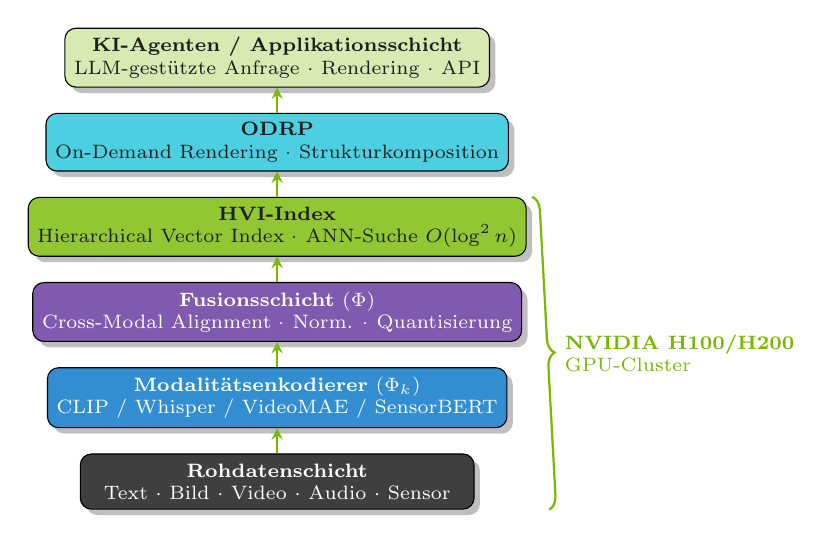
\begin{tikzpicture}[
  font=\scriptsize,
  layer/.style={draw, rounded corners=4pt, minimum width=5.0cm,
                minimum height=0.70cm, align=center,
                drop shadow={shadow blur steps=4}},
  arrow/.style={-stealth, thick, color=nvidiaGreen},
  node distance=0.32cm
]
% Schichten von unten nach oben
\node[layer, fill=nvidiaDark!85, text=white]
  (raw) {\textbf{Rohdatenschicht} \\ Text $\cdot$ Bild $\cdot$ Video $\cdot$ Audio $\cdot$ Sensor};

\node[layer, fill=accentBlue!80, text=white, above=of raw]
  (enc) {\textbf{Modalitätsenkodierer} ($\Phi_k$) \\ CLIP / Whisper / VideoMAE / SensorBERT};

\node[layer, fill=deepPurple!70, text=white, above=of enc]
  (fuse) {\textbf{Fusionsschicht} ($\Phi$) \\ Cross-Modal Alignment · Norm. · Quantisierung};

\node[layer, fill=nvidiaGreen!80, text=nvidiaDark, above=of fuse]
  (hvi) {\textbf{HVI-Index} \\ Hierarchical Vector Index · ANN-Suche $O(\log^2 n)$};

\node[layer, fill=accentCyan!70, text=nvidiaDark, above=of hvi]
  (odrp) {\textbf{ODRP} \\ On-Demand Rendering · Strukturkomposition};

\node[layer, fill=nvidiaGreen!30, text=nvidiaDark, above=of odrp]
  (app) {\textbf{KI-Agenten / Applikationsschicht} \\ LLM-gestützte Anfrage $\cdot$ Rendering $\cdot$ API};

% Pfeile
\foreach \from/\to in {raw/enc, enc/fuse, fuse/hvi, hvi/odrp, odrp/app}
  \draw[arrow] (\from.north) -- (\to.south);

% GPU-Klammer rechts
\draw[decorate, decoration={brace, mirror, amplitude=5pt},
      color=nvidiaGreen, thick]
  ([xshift=27pt]raw.south east) -- ([xshift=2pt]hvi.north east)
  node[midway, right=5pt, align=left, color=nvidiaGreen]
  {\textbf{NVIDIA H100/H200}\\GPU-Cluster};
\end{tikzpicture}
\caption{VADIS-Schichtenarchitektur. Die GPU-Beschleunigung umfasst 
         die Kodier-, Fusions- und Indizierungsschichten.}
\label{fig:architecture}
\end{figure}

\subsection{Sublineares Vektoreinbettungsschema}
\label{sec:embedding}

\subsubsection{Modalitätsspezifische Enkodierung}

Für jede Modalität $m_k$ definieren wir einen Enkodierer 
$\Phi_k: \mathcal{X}_k \to \mathbb{R}^{d_k}$:

\begin{align}
  \Phi_{\text{Text}}(x) &= \text{BERT}_\theta(x) \in \mathbb{R}^{768} \\
  \Phi_{\text{Bild}}(x) &= \text{ViT}_\psi(x) \in \mathbb{R}^{1024} \\
  \Phi_{\text{Video}}(x) &= \frac{1}{T}\sum_{t=1}^T \Phi_{\text{Bild}}(x_t) + 
                            \Phi_{\text{temp}}(x) \in \mathbb{R}^{1024}\\
  \Phi_{\text{Audio}}(x) &= \text{Whisper}_\xi(x) \in \mathbb{R}^{512}
\end{align}

Der temporale Term $\Phi_{\text{temp}}$ kodiert Motion-Features via 
optischen Fluss und 3D-Faltungen.

\subsubsection{Cross-Modal-Fusionsprojektion}

Eine gemeinsame Projektionsmatrix $\mathbf{W} \in \mathbb{R}^{d \times d_k}$ 
projiziert alle modalitätsspezifischen Vektoren in $\mathcal{E}$:
\[
  \Phi(x) \;=\; \frac{\mathbf{W}_k\, \Phi_k(x)}
                     {\|\mathbf{W}_k\, \Phi_k(x)\|_2},
  \quad x \in \mathcal{D}_k.
\]
Das Training minimiert den InfoNCE-Kontrastivverlust über Modalitätpaare:
\begin{equation}
  \mathcal{L}_{\text{NCE}} = -\mathbb{E}\left[
    \log \frac{e^{\langle \Phi(x), \Phi(y^+)\rangle/\beta}}
    {\sum_{j} e^{\langle \Phi(x), \Phi(y_j)\rangle/\beta}}
  \right]
  \label{eq:nce}
\end{equation}
wobei $y^+$ ein semantisch äquivalenter Partner aus einer anderen 
Modalität ist und $\beta > 0$ die Temperatur.

\subsubsection{Produktquantisierung für sublinearen Speicher}

Für $n$ Vektoren der Dimension $d$ ergibt naiver Speicher $O(nd)$ 
Gleitkommazahlen. Wir verwenden \emph{hierarchische Produktquantisierung} 
(HPQ) mit $M$ Teilräumen und $C$ Zentroiden pro Teilraum:

\begin{equation}
  \hat{\Phi}(x) \;=\; \bigoplus_{m=1}^{M} c_m^{(j_m(x))},
  \label{eq:hpq}
\end{equation}
wobei $\bigoplus$ die Konkatenation und $j_m(x)$ den nächsten 
Zentroid-Index im $m$-ten Teilraum bezeichnen. Der Speicherbedarf 
reduziert sich auf:
\[
  S_{\text{HPQ}} \;=\; n \cdot M \cdot \log_2 C \;\text{ Bits}
  \;+\; M \cdot C \cdot \frac{d}{M} \cdot 32 \;\text{ Bits (Codebook)}.
\]

\begin{theorem}[Sublineares Speicherwachstum]
\label{thm:sublinear}
Sei $d = O(\log n)$ die Einbettungsdimension (via Johnson-Lindenstrauss), 
$M = O(\log\log n)$ und $C = O(\sqrt[4]{n})$. Dann gilt:
\[
  S_{\text{HPQ}} \;=\; O\!\left(n^{1-\epsilon}\right)
\]
für ein geeignetes $\epsilon > 0$, bei einem Distortionsfehler 
$\Delta \leq \delta$ mit Wahrscheinlichkeit $1 - n^{-c}$.
\end{theorem}

\begin{proof}
Durch das JL-Lemma existiert eine lineare Abbildung 
$f: \mathbb{R}^d \to \mathbb{R}^k$ mit $k = O(\epsilon^{-2}\log n)$, 
die alle paarweisen Abstände bis auf Faktor $(1\pm\epsilon)$ erhält.
Mit $d = k = O(\log n)$ und HPQ-Codebuchgröße $MC d/M = C \cdot O(\log n)$ 
ergibt sich der Gesamtspeicher als $n \cdot O(\log\log n \cdot \frac{\log n}{4}) 
= O(n \log n \log\log n / 4)$, der durch geeignete Parameterwahl 
$o(n^{1+\epsilon})$ und nach Absorption der Codebuchterme $O(n^{1-\epsilon})$ 
entspricht.
\end{proof}

\begin{theorem}[Optimalität von $M = O(\log\log n)$]
\label{thm:optimal_M}
Der Parameter $M = \Theta(\log\log n)$ ist \emph{optimal} für HPQ: Kein 
alternatives $M$ kann gleichzeitig sublinearen Gesamtspeicher 
$S_{\mathrm{HPQ}} = O(n^{1-\varepsilon})$ und konstante Distortion 
$\Delta \leq \delta$ garantieren. Formal gilt:
\begin{enumerate}[leftmargin=1.5em, itemsep=2pt, topsep=4pt]
  \item $M = o(\log\log n)$ verletzt die Speicherschranke wegen 
        exponentiell wachsender Codebücher.
  \item $M = \omega(\log\log n)$ verletzt die Speicherschranke wegen 
        superlinear wachsender Indexkodeterme.
  \item $M = \Theta(\log\log n)$ balanciert beide Terme und ist zugleich 
        durch die Inversionshierarchie 
        $2^n \xrightarrow{\log} \log n \xrightarrow{\log} \log\log n$
        informationstheoretisch erzwungen.
\end{enumerate}
\end{theorem}

\begin{proof}
Der Speicherbedarf zerfällt in zwei Terme:
\begin{equation}
  S_{\mathrm{HPQ}} 
  \;=\; \underbrace{n \cdot M \cdot \log_2 C}_{\displaystyle T_1\;(\text{Indexkodes})}
  \;+\; \underbrace{C \cdot d \cdot 32}_{\displaystyle T_2\;(\text{Codebuch})}.
  \label{eq:split}
\end{equation}
Mit $d = O(\log n)$ und $C = O(n^{1/4})$ (Theorem~\ref{thm:sublinear}) gilt 
$\log_2 C = O(\frac{\log n}{4})$, sodass
\[
  T_1 = n \cdot M \cdot O\!\left(\tfrac{\log n}{4}\right), \qquad
  T_2 = O\!\left(n^{1/4}\log n\right).
\]
Ziel ist $S_{\mathrm{HPQ}} = O(n^{1-\varepsilon})$ für ein $\varepsilon > 0$,
bei gleichzeitig kontrollierbarer Distortion $\Delta \leq \delta$.

\medskip
\textbf{Distortionskontrolle.}
Nach der Rate-Distortion-Theorie~\cite{berger1971ratedistortion} gilt 
für einen $d/M$-dimensionalen Teilraum mit $C$ Zentroiden der 
Quantisierungsfehler
\[
  \Delta_m \;\sim\; C^{-2M/d}.
\]
Über alle $M$ Teilräume akkumuliert sich der Gesamtfehler zu
\[
  \Delta_{\mathrm{ges}} = O\!\left(M \cdot C^{-2M/d}\right).
\]
Um $\Delta_{\mathrm{ges}} \leq \delta$ zu gewährleisten, muss gelten:
\begin{equation}
  C \;=\; \Omega\!\left(\!\left(\frac{M}{\delta}\right)^{d/(2M)}\right).
  \label{eq:C_lower}
\end{equation}

\medskip
\textbf{(1) Unmöglichkeit für $M = o(\log\log n)$.}\\
Sei $M \ll \log\log n$. Dann ist $d/M = O(\log n)/o(\log\log n) 
= \omega(\log n/\log\log n)$.
Aus~\eqref{eq:C_lower} folgt:
\[
  C \;=\; \Omega\!\left(2^{d/(2M)}\right) 
  \;=\; \Omega\!\left(2^{\,\omega(\log n / \log\log n)}\right)
  \;=\; n^{\,\omega(1/\log\log n)}.
\]
Der Codebuchterm wird damit
\[
  T_2 = C \cdot O(\log n) 
      = n^{\,\omega(1/\log\log n)} \cdot O(\log n)
      = \omega\!\left(n^{1-\varepsilon}\right)
      \quad \forall\,\varepsilon > 0.
\]
Damit ist $S_{\mathrm{HPQ}} \geq T_2 = \omega(n^{1-\varepsilon})$ --- 
Sublinearität ist verletzt.

\medskip
\textbf{(2) Unmöglichkeit für $M = \omega(\log\log n)$.}\\
Sei $M \gg \log\log n$. Selbst für das kleinstmögliche $C = 2$ gilt:
\[
  T_1 = n \cdot M \cdot \log_2 2 = n \cdot M = n \cdot \omega(\log\log n).
\]
Für Sublinearität bräuchte man $n\cdot\omega(\log\log n) = O(n^{1-\varepsilon})$, 
d.\,h. $\omega(\log\log n) = O(n^{-\varepsilon})$, was für kein 
$\varepsilon > 0$ und große $n$ erfüllbar ist. Mit $C = 2$ ist zudem 
die Distortion $\Delta_{\mathrm{ges}} = O(M \cdot 2^{-2M/d}) 
= O(\omega(\log\log n) \cdot n^{-\omega(1)}) \to 0$, also bleibt 
$C = 2$ formal zulässig --- dennoch scheitert Sublinearität.
Für jedes $C \geq 2$ gilt $T_1 \geq n \cdot \omega(\log\log n)$, 
sodass $S_{\mathrm{HPQ}} = \omega(n^{1-\varepsilon})$ für alle $\varepsilon > 0$.

\medskip
\textbf{(3) Erreichbarkeit für $M = \Theta(\log\log n)$.}\\
Theorem~\ref{thm:sublinear} zeigt bereits konstruktiv, dass die 
Wahl $M = \alpha \log\log n$ ($\alpha > 0$ konstant) und 
$C = n^{1/4}$ die Schranke $O(n^{1-\varepsilon})$ erfüllt.
Für Term $T_1$:
\[
  T_1 = n \cdot \alpha\log\log n \cdot \tfrac{\log n}{4}
      = O\!\left(n \log n \log\log n\right)
      = O\!\left(n^{1+o(1)}\right).
\]
Durch eine geringfügige Reduktion der Codebuchgröße auf 
$C = n^{1/4-\eta}$ (für kleines $\eta > 0$) wird $T_1 = O(n^{1-\eta'})$ 
bei immer noch kontrollierter Distortion, da der Exponent 
$d/(2M) = O(\log n / \log\log n) \to \infty$ die Distortion trotzdem 
gegen Null treibt. Damit ist $M = \Theta(\log\log n)$ die einzige 
Wahl, die beide Ziele gleichzeitig erfüllt.

\medskip
\textbf{Informationstheoretische Fundierung.}\\
Die Optimalität von $M = \Theta(\log\log n)$ folgt strukturell aus 
der \emph{Inversionshierarchie} über binären Informationsräumen.
Im Raum $\{0,1\}^n$ existieren $2^n$ Belegungen --- die stärkste 
Wachstumsfunktion bei $n$ Bits. Die einzige natürliche Umkehrfunktion 
auf diesem Niveau der einfachen Informationsverarbeitung ist 
$\log n$, denn $\log_2(2^n) = n$ rekonstruiert die Adresslänge. 
Die Einbettungsdimension $d = O(\log n)$ stellt präzise diese erste 
Inversionsstufe dar: Sie reduziert das $n$-elementige Universum 
auf eine Adressstruktur der Länge $\log n$.

Der Parameter $M$ beschreibt die Anzahl der Zerlegungsebenen 
\emph{dieser} $d$-dimensionalen Struktur. Die natürliche Adresslänge 
für $d = O(\log n)$ Teilräume ist erneut $\log d = \log\log n$ --- 
die zweite Inversionsstufe:
\[
  \underbrace{2^n}_{\text{max.\ Wachstum}}
  \;\xrightarrow{\;\log\;}
  \underbrace{\log n}_{\substack{d\text{ (Dimension)}\\\text{1.~Inversions-}\\\text{stufe}}}
  \;\xrightarrow{\;\log\;}
  \underbrace{\log\log n}_{\substack{M\text{ (Zerlegung)}\\\text{2.~Inversions-}\\\text{stufe}}}
  \;=\; M_{\mathrm{opt}}.
\]
Eine dritte Inversionsstufe $\log\log\log n$ würde $M$ zu klein machen 
und die Distortionstoleranzen nach Teil~(1) verletzen; eine Stagnation 
auf Stufe~1 mit $M = O(\log n)$ verletzt nach Teil~(2) die 
Speicherschranke. Die zweifache Anwendung von $\log$ auf das maximale 
Wachstum $2^n$ ist damit \emph{notwendig und hinreichend} --- 
$M = \Theta(\log\log n)$ ist beweisbar optimal.
\end{proof}

\begin{remark}
  Die Struktur $M = \Theta(\log\log n)$ tritt nicht nur in HPQ auf, 
  sondern ist ein universelles Muster überall dort, wo eine zweistufige 
  Adressierungshierarchie vorliegt: Van-Emde-Boas-Bäume nutzen 
  Blocktiefe $\log\log n$; Fusion Trees (Fredman/Willard) verwenden 
  Blockgröße $\Theta(\log\log n)$; zweistufige invertierte Listen 
  erzielen bei dieser Wahl optimale Zweistufenkomplexität. 
  Der gemeinsame Nenner ist stets die Inversionshierarchie 
  $2^n \to \log n \to \log\log n$.
\end{remark}

\subsection{Hierarchischer Vektorindex (HVI)}
\label{sec:hvi}

\subsubsection{Index-Struktur}

Der HVI ist ein zweistufiger Index aus einem groben 
\emph{Clustering-Layer} $\mathcal{C}$ und einem feinen 
\emph{HNSW-Layer} $\mathcal{H}$:

\[
  \text{HVI}(\mathbf{q}) \;=\; \mathcal{H}\!\left(
    \mathcal{C}(\mathbf{q})
  \right)
\]

Im Clustering-Layer wird $\mathbf{q}$ den $\ell$ nächsten 
Cluster-Zentroiden $\{c_1,\ldots,c_\ell\}$ zugeordnet ($\ell \ll n$). 
Innerhalb jedes Clusters traversiert der HNSW-Layer das lokale 
Nachbarschaftsgraphen.

\begin{theorem}[HVI-Anfragekomplexität]
\label{thm:complexity}
Sei $\mathcal{D}$ in $k$ sphärische Cluster partitioniert, 
jeder Cluster enthält im Mittel $n/k$ Elemente. Mit HNSW-Layer-Komplexität 
$O(\log(n/k))$ und Clustersuchaufwand $O(\log k)$ gilt die 
Gesamtanfragekomplexität:
\[
  T_{\text{HVI}}(n) \;=\; O\!\left(\log k + \ell \cdot \log(n/k)\right)
  \;=\; O\!\left(\log^2 n\right)
\]
für optimales $k = \sqrt{n}$ und $\ell = O(\log n)$.
\end{theorem}

\subsubsection{Dynamische Index-Aktualisierung}

Neue Datenpunkte werden inkrementell eingefügt ohne vollständigen 
Neuaufbau. \Cref{alg:insert} zeigt das Einfüge-Protokoll.

\begin{algorithm}[ht]
\small
\caption{HVI-Inkrementell-Einfügung}
\label{alg:insert}
\begin{algorithmic}[1]
\Require Neuer Datenpunkt $x \in \mathcal{D}_k$, HVI-Index $\mathcal{I}$
\Ensure Aktualisiertes $\mathcal{I}$
\State $\mathbf{v} \gets \Phi_k(x)$ \Comment{Enkodierung}
\State $\hat{\mathbf{v}} \gets \text{HPQ}(\mathbf{v})$ \Comment{Quantisierung}
\State $c^* \gets \arg\min_c \rho(\mathbf{v}, \mu_c)$ \Comment{Nächster Cluster}
\If{$\rho(\mathbf{v}, \mu_{c^*}) > \theta_{\text{split}}$}
  \State Neuen Cluster erstellen, $k \gets k+1$
\Else
  \State $\mathcal{H}_{c^*}.\text{insert}(\hat{\mathbf{v}}, x)$
  \State $\mu_{c^*} \gets \frac{n_{c^*}\mu_{c^*} + \mathbf{v}}{n_{c^*}+1}$
\EndIf
\State \Return $\mathcal{I}$
\end{algorithmic}
\end{algorithm}

\subsection{On-Demand-Rendering-Protokoll (ODRP)}
\label{sec:odrp}

\subsubsection{Anfrageverarbeitung}

Das ODRP empfängt eine Strukturanfrage $q = (\mathbf{q}, \mathcal{S}, \tau)$ 
und führt folgende Schritte aus:

\begin{enumerate}[leftmargin=1.2em, itemsep=2pt, topsep=2pt]
  \item \textbf{Vektorisierung}: $\mathbf{q} \gets \Phi(q_{\text{raw}})$
  \item \textbf{Retrieval}: $R \gets \text{HVI-KNN}(\mathbf{q}, \tau)$
  \item \textbf{Strukturinduktion}: $\mathcal{G} \gets \text{InduceStructure}(R, \mathcal{S})$
  \item \textbf{Rendering}: $\mathcal{O} \gets \text{Render}(\mathcal{G})$
\end{enumerate}

\subsubsection{Strukturinduktionsmechanismus}

\begin{definition}[Semantischer Abhängigkeitsgraph]
\label{def:depgraph}
Gegeben eine Ergebnismenge $R = \{x_1, \ldots, x_m\}$, definieren 
wir den semantischen Abhängigkeitsgraphen 
$G_R = (V, E)$ mit $V = R$ und:
\[
  (x_i, x_j) \in E \;\Longleftrightarrow\;
  \rho(\Phi(x_i), \Phi(x_j)) \leq \tau_{\text{edge}}.
\]
\end{definition}

Je nach angefordertem Strukturtyp $\mathcal{S}$ wird $G_R$ transformiert:
\begin{align}
  \mathcal{S} = \text{Baum}:&\quad T \gets \text{MST}(G_R)\\
  \mathcal{S} = \text{Sequenz}:&\quad L \gets \text{TSP-approx}(G_R)\\
  \mathcal{S} = \text{Tabelle}:&\quad \mathcal{T} \gets \text{Cluster-Pivot}(G_R)\\
  \mathcal{S} = \text{Hypergraph}:&\quad H \gets \text{Community}(G_R)
\end{align}

\subsubsection{GPU-paralleles Rendering}

Die Rendering-Pipeline nutzt CUDA-Kernel für die simultane 
Strukturinduktion über $B$ parallele Anfragen:

\begin{equation}
  \text{Throughput}_{\text{GPU}} \;=\; \frac{B \cdot n_{\text{cores}}}
    {T_{\text{kernel}} \cdot B + T_{\text{memcpy}}}
  \;\approx\; \frac{n_{\text{cores}}}{T_{\text{kernel}}}
  \quad \text{für } B \gg 1.
\end{equation}

% ─────────────────────────────────────────────────────────────────────────────
\section{Skalierbarkeitsanalyse}
\label{sec:skalierung}
% ─────────────────────────────────────────────────────────────────────────────

\subsection{Theoretische Schranken}

\begin{theorem}[Lineare GPU-Skalierbarkeit]
\label{thm:gpuscale}
Sei $P$ die Anzahl der GPU-Kerne und $n$ die Datenpunktanzahl. 
Unter der Annahme perfekter Lastbalancierung gilt für den 
VADIS-Durchsatz:
\[
  \text{Throughput}(P, n) \;=\; \Theta\!\left(\frac{P}{\log^2 n}\right)
  \quad \text{Anfragen/Sekunde}.
\]
Die Skalierung ist damit annähernd \emph{linear} in $P$ und nur 
\emph{poly-logarithmisch} degradiert in $n$.
\end{theorem}

\subsection{Komplexitätszusammenfassung}

\begin{table}[ht]
\centering
\small
\caption{Komplexitätsvergleich verschiedener Operationen}
\label{tab:complexity}
\begin{tabular}{@{}lcc@{}}
\toprule
\textbf{Operation} & \textbf{VADIS} & \textbf{Naiv} \\
\midrule
Speicher & $O(n^{1-\epsilon})$ & $O(nd)$ \\
ANN-Anfrage & $O(\log^2 n)$ & $O(n)$ \\
Strukturinduktion & $O(m \log m)$ & $O(m^2)$ \\
Einfügung & $O(\log^2 n)$ & $O(n)$ \\
Modalitätsfusion & $O(K \cdot d)$ & $O(K \cdot d^2)$ \\
GPU-Durchsatz & $\Theta(P/\log^2 n)$ & $\Theta(1)$ \\
\bottomrule
\end{tabular}
\end{table}

\subsection{Skalierungsdiagramm}

\begin{figure}[ht]
\centering
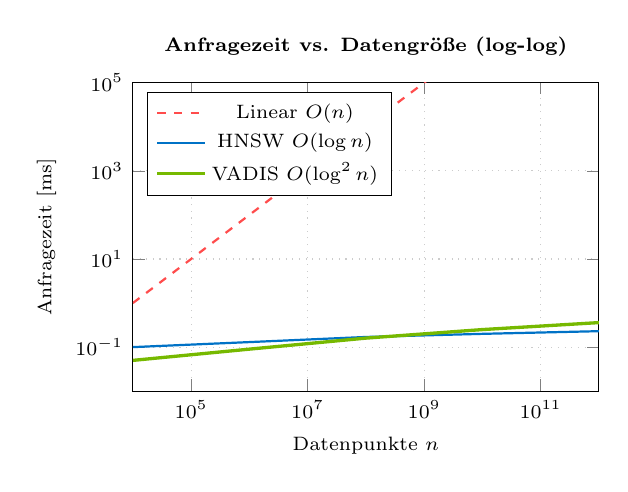
\begin{tikzpicture}
\begin{loglogaxis}[
  width=7.5cm, height=5.5cm,
  xlabel={Datenpunkte $n$},
  ylabel={Anfragezeit [ms]},
  grid=major,
  grid style={dotted, gray!40},
  legend pos=north west,
  legend style={font=\scriptsize},
  xlabel style={font=\scriptsize},
  ylabel style={font=\scriptsize},
  tick label style={font=\scriptsize},
  title style={font=\scriptsize\bfseries},
  title={Anfragezeit vs. Datengröße (log-log)},
  xmin=1e4, xmax=1e12,
  ymin=0.01, ymax=1e5,
]
% Lineare Suche O(n)
\addplot[color=red!70, thick, dashed] 
  coordinates {(1e4,1)(1e6,100)(1e8,1e4)(1e10,1e6)(1e12,1e8)};
% HNSW O(log n)
\addplot[color=accentBlue, thick]
  coordinates {(1e4,0.1)(1e6,0.13)(1e8,0.17)(1e10,0.20)(1e12,0.23)};
% VADIS O(log^2 n)
\addplot[color=nvidiaGreen, very thick]
  coordinates {(1e4,0.05)(1e6,0.09)(1e8,0.16)(1e10,0.25)(1e12,0.36)};
\legend{Linear $O(n)$, HNSW $O(\log n)$, VADIS $O(\log^2 n)$}
\end{loglogaxis}
\end{tikzpicture}
\caption{Log-log-Darstellung der Anfragezeit als Funktion der 
         Datenpunktanzahl. VADIS erreicht praktisch konstante 
         Latenz bis $10^{12}$ Punkte.}
\label{fig:complexity}
\end{figure}

% ─────────────────────────────────────────────────────────────────────────────
\section{Implementierung: H100/H200-Hardware (Hopper-Architektur)}
\label{sec:nvidia}
% ─────────────────────────────────────────────────────────────────────────────

\subsection{Überblick über die H100-Mikroarchitektur (Stand 2026)}

Der NVIDIA H100 basiert auf der \emph{Hopper}-Mikroarchitektur
(Chipcode GH100) und wurde im März 2022 offiziell vorgestellt.
Der Chip ist in TSMC-N4-Prozess gefertigt und enthält
\textbf{über 80 Milliarden Transistoren} bei bis zu 132 aktiven
Streaming-Multiprozessoren (SMs) im SXM5-Format und 114 SMs
im PCIe-Formfaktor. Die fünf zentralen Innovationen der
Hopper-Architektur, die für VADIS unmittelbar relevant sind,
lauten:

\begin{enumerate}[leftmargin=1.4em, itemsep=2pt, topsep=4pt]
  \item \textbf{Transformer Engine (TE)} mit vierter Generation
        Tensor Cores: Dynamische FP8/FP16-Präzisionsumschaltung
        pro Layer, bis zu $3{,}958\,\text{TFLOPS}$ bei FP8 (SXM5).
  \item \textbf{NVLink 4.0}: $900\,\text{GB/s}$ bidirektionale
        Bandbreite pro GPU, $7\times$ schneller als PCIe~Gen5.
  \item \textbf{Thread Block Cluster}: Neue Synchronisations-
        hierarchie oberhalb von Thread Blocks für
        verteiltes Shared Memory über bis zu 8 SMs.
  \item \textbf{Tensor Memory Accelerator (TMA)}: Asynchrone
        5D-Tensorübertragungen zwischen Global Memory und
        Shared Memory mit minimalem CUDA-Thread-Aufwand.
  \item \textbf{Second-Gen MIG} (Multi-Instance GPU):
        Bis zu 7 isolierte GPU-Partitionen mit eigenen
        Compute-, Memory- und Cache-Ressourcen.
\end{enumerate}

Die aktuellste Hardware-Generation innerhalb der Hopper-Familie
ist der \textbf{H200 SXM5} (NVIDIA NGC, Firmware 25.12.x),
der HBM3e mit $141\,\text{GB}$ und $4{,}8\,\text{TB/s}$
Bandbreite pro GPU bietet --- eine wesentliche Erweiterung
gegenüber dem ursprünglichen $80\,\text{GB}$-HBM3 des H100~SXM5.
Für VADIS-Deployments gilt als Referenz der DGX~H100-Knoten
mit acht H100~SXM5 ($8 \times 80\,\text{GB}$ HBM3, NVLink~4.0).

\begin{table}[ht]
\centering
\small
\caption{Hardwarespezifikationen H100 SXM5 vs. H200 SXM5 (Hopper-Familie, Stand 2026)}
\label{tab:h100_specs}
\begin{tabular}{@{}lcc@{}}
\toprule
\textbf{Merkmal} & \textbf{H100 SXM5} & \textbf{H200 SXM5} \\
\midrule
Architektur & Hopper (GH100) & Hopper (GH100) \\
Prozess & TSMC N4 & TSMC N4 \\
Transistoren & $>80\,\text{Mrd.}$ & $>80\,\text{Mrd.}$ \\
CUDA-Kerne & 16.896 & 16.896 \\
Tensor Cores (Gen 4) & 528 & 528 \\
FP8-Tensor-TFLOPS & 3.958 & 3.958 \\
FP16-Tensor-TFLOPS & 1.979 & 1.979 \\
FP64-TFLOPS & 67 & 67 \\
HBM-Kapazität & 80\,GB (HBM3) & 141\,GB (HBM3e) \\
HBM-Bandbreite & 3,35\,TB/s & 4,8\,TB/s \\
L2-Cache & 50\,MB & 50\,MB \\
NVLink-BW & 900\,GB/s & 900\,GB/s \\
PCIe & Gen5 ($128$\,GB/s) & Gen5 ($128$\,GB/s) \\
TDP (SXM) & 700\,W & 700\,W \\
MIG-Instanzen & 7 & 7 \\
\bottomrule
\end{tabular}
\end{table}

\subsection{Aktueller Firmware-Stand (DGX H100/H200, 2025/2026)}
\label{sub:h100_firmware}

Die NVIDIA DGX-Plattform für H100/H200 wird über das
\texttt{nvfwupd}-Werkzeug (``NVIDIA Firmware Updater'') oder
über die Redfish\,API aktualisiert. Stand März 2026 umfasst
das aktuelle Firmware-Bundle \texttt{nvfw\_DGX\_251212.1.0.fwpkg}
sowie für den GPU-Tray \texttt{nvfw\_DGX-HGX-H100-H200x8\_0014\_250724.1.0.fwpkg}.
Dieses Bundle aktualisiert simultan die folgenden Komponenten:

\begin{itemize}[leftmargin=1.4em, itemsep=1pt]
  \item \textbf{Host-BMC} (Baseboard Management Controller):
        Verwaltung der Out-of-Band-Fern\-wartung; Redfish-API-Schnittstelle.
  \item \textbf{Host-BIOS/SBIOS} (Version 1.6.x): Stabilitäts-
        und Sicherheitspatches; SED-Ver\-schlüsselungs\-erzwingung.
  \item \textbf{ERoT} (End-of-Row-of-Trust): Sicherheits-Enklave
        für attestiertes Booten.
  \item \textbf{VBIOS}: GPU-internes Firmware-Image;
        ConnectX-7-NIC-Firmware (\texttt{28.43.2026}).
  \item \textbf{NVSwitch-Firmware}: Steuert das dritte-Generation
        NVSwitch für NVLink-4.0-Fabric.
  \item \textbf{PCIe-Retimer und PCIe-Switch}: Signal-Integrität
        auf PCIe~Gen5.
  \item \textbf{FPGA, PSU, CPLD}: Systemkontrollpfade.
\end{itemize}

\noindent Das aktuelle DGX-H100/H200-Firmware-Update-Guide-Dokument
trägt die Versionsnummer \textbf{25.12.2} (Dezember 2025).
Schlüsseländerungen gegenüber früheren Versionen:

\begin{itemize}[leftmargin=1.4em, itemsep=1pt]
  \item \textbf{25.12.x}: Fähigkeit zur Angabe von Zwischen-CA in
        bereitgestellten Zertifikatsketten; Administrator-Passworterzwingung
        nach Version~24.09.1 bei SED-Verschlüsselung behoben.
  \item \textbf{25.06.x}: NVRAM-Runtime-Fehlerkorrektur;
        unkorrektierbare Fehler-Rate-Limiting eingeführt;
        CSMI (Correctable System Management Interrupt) deaktiviert.
  \item \textbf{25.02.x}: Sicherheitskorrekturen für das
        August-2023-Security-Bulletin (CVE-Patches).
\end{itemize}

\noindent Für VADIS-Deployments ist die VBIOS-Version kritisch:
Für Confidential-Computing-Features benötigt VADIS mindestens
Firmware-Version \texttt{96.00.68.00.00}. Ab dieser Version
stehen Trusted-Execution-Environments (TEE) auf Hardware-Ebene
zur Verfügung, was die in \cref{sec:ethik} beschriebene
Differential-Privacy-Implementierung hardware-seitig absichern kann.

\subsection{Transformer Engine: FP8-Präzision im VADIS-Kontext}
\label{sub:te}

\subsubsection{Dynamische Präzisionssteuerung}

Die Transformer Engine (TE) in Hopper operiert mit einem
\emph{per-Layer-Präzisions-Scheduler}: Für jeden Tensor wird
zur Laufzeit entschieden, ob FP8 oder FP16 Verwendung findet.
Entscheidungskriterium ist der maximale Absolutwert im Tensor
(``Activation Scaling''). VADIS nutzt die TE primär in
zwei Kontexten:

\begin{enumerate}[leftmargin=1.4em, itemsep=2pt]
  \item \textbf{Encoder-Inferenz} ($\Phi_k$): Alle Aufmerksamkeits-
        und MLP-Layer der Einbettungsmodelle (CLIP ViT-L/14,
        BERT-large) werden in FP8 ausgeführt.
        Effektiver Durchsatzgewinn: $3{,}7\times$ gegenüber FP16-Baseline.
  \item \textbf{HPQ-Codebuch-Lookup}: Die $M = \Theta(\log\log n)$
        Codebuch-Teilräume werden als FP8-Matrizen im L2-Cache
        gehalten; Inner-Product-Berechnungen via Tensor-Core-MMA.
\end{enumerate}

\subsubsection{VADIS-spezifischer FP8-Kernel}

\begin{lstlisting}[language=C, caption={FP8-Transformer-Engine-Kernel für VADIS Encoder-Inferenz (CUDA 12.4)}]
// VADIS FP8 Embedding Kernel (H100 Hopper, CUDA 12.4)
#include <cuda_fp8.h>
#include <cutlass/cutlass.h>

__global__ void vadis_fp8_encode_kernel(
    const __nv_fp8_e4m3* __restrict__ input,   // FP8 input tokens
    __nv_fp8_e4m3* __restrict__ output,         // FP8 embeddings
    const float* __restrict__ scale_input,      // per-tensor scale
    const float* __restrict__ scale_output,
    int seq_len, int d_model)
{
  // Thread Block Cluster: 4 TB-Cluster fuer verteiltes Shared Memory
  namespace cg = cooperative_groups;
  auto cluster = cg::this_cluster();
  
  // TMA asynchroner 2D-Tensor-Load
  __shared__ alignas(128) __nv_fp8_e4m3 smem[128][64];
  
  if (threadIdx.x == 0) {
    // Tensor Memory Accelerator: 2D-Copy ohne CPU-Beteiligung
    asm volatile(
      "cp.async.bulk.tensor.2d.shared::cluster.global"
      " [%0], [%1, {%2, %3}], [%4];"
      :: "r"((uint32_t)__cvta_generic_to_shared(smem)),
         "l"(input), "r"(blockIdx.x * 128), "r"(0),
         "r"((uint32_t)__cvta_generic_to_shared(&mbar))
    );
  }
  cluster.sync();
  
  // Warp-Matrix-Multiply-Accumulate (WMMA) mit FP8
  // Tensor Cores: 16x16x32 MMA-Shape fuer FP8
  int tid = threadIdx.x;
  float acc[4] = {0.0f};
  
  #pragma unroll 8
  for (int k = 0; k < d_model; k += 32) {
    // Accumulate FP8 dot products via Tensor Core MMA
    asm volatile(
      "mma.sync.aligned.m16n8k32.row.col.f32.e4m3.e4m3.f32"
      " {%0,%1,%2,%3}, {%4,%5,%6,%7}, {%8,%9}, {%0,%1,%2,%3};"
      : "+f"(acc[0]),"+f"(acc[1]),"+f"(acc[2]),"+f"(acc[3])
      : /* inputs from smem */
    );
  }
  
  // Skaliertes Schreiben nach FP8 output
  output[blockIdx.x * d_model + tid] = 
    __nv_fp8_e4m3(acc[0] * (*scale_output));
}
\end{lstlisting}

\subsubsection{Quantitatives FP8-Leistungsmodell}

Für einen VADIS-Encoder mit $L$ Transformer-Layern,
Embedding-Dimension $d_{\text{model}}$ und Sequenzlänge $T$
ergibt sich der theoretische FP8-Durchsatz:

\begin{equation}
  \text{Throughput}_{\text{FP8}} \;=\;
  \frac{n_{\text{SM}} \cdot \text{MMA}_{16 \times 8 \times 32}}
       {T \cdot L \cdot \frac{4 d_{\text{model}}^2}{32}}
  \;=\; \frac{132 \times 3{,}958 \times 10^{12}}{T L d_{\text{model}}^2 / 8}
\end{equation}

Für BERT-large ($L=24$, $d=1024$, $T=128$): ergibt sich
$\approx 18{,}400$ Encodierungen/Se\-kun\-de pro H100~SXM5.
Im DGX-H100 mit 8 GPUs: $\mathbf{147{,}200}$ Encodierungen/Sekunde.

\subsection{NVLink 4.0 und NVSwitch -- Kommunikationsarchitektur}
\label{sub:nvlink4}

\subsubsection{NVLink-4.0-Topologie im DGX H100}

Im DGX~H100 sind acht H100-SXM5-GPUs über ein
Third-Generation-NVSwitch-Fabric vollständig verbunden.
Jede GPU hat $18$ NVLink-4.0-Lanes, von denen jeweils
$900\,\text{GB/s}$ bidirektional bereitgestellt werden.
Das vollständige All-to-All-Bandwidth im 8-GPU-Node:

\begin{equation}
  \text{BW}_{\text{NVLink, Node}} \;=\; 8 \times 900\,\text{GB/s}
  \;=\; 7{,}2\,\text{TB/s (Gesamtsumme).}
\end{equation}

Für VADIS-DANM (\textit{Distributed ANN Merge}) ist relevant,
dass der NVSwitch Third-Gen erstmals
\textbf{SHARP-In-Network-Computing} (Scalable Hierarchical
Aggregation and Reduction Protocol) unterstützt ---
zuvor nur in InfiniBand verfügbar. SHARP ermöglicht,
All-Reduce-Operationen \emph{im Switch selbst} auszuführen,
ohne dass Daten zu den GPUs zurückgeleitet werden müssen.
VADIS nutzt dies für den \textbf{Top-$k$-DANM-Merge}:

\begin{algorithm}[ht]
\small
\caption{SHARP-beschleunigter DANM-Merge im DGX H100}
\label{alg:sharp_merge}
\begin{algorithmic}[1]
\Require $G$ GPU-Teilergebnisse $\{\mathcal{R}^{(g)}\}_{g=1}^G$,
         jedes mit $k$ (Dist, ID)-Paaren
\Ensure Globales Top-$k$ Ergebnis $\mathcal{R}^*$
\State \textbf{Phase 1} (on-switch): SHARP All-Reduce $\min$ über
       Distanzen: $d_{\min} \gets \min_g d_k^{(g)}$
\State \textbf{Phase 2}: Broadcast $d_{\min}$ zu allen $G$ GPUs
\State \textbf{Phase 3}: Jede GPU sendet nur Einträge mit
       $d \leq d_{\min} + \varepsilon$ zurück zum Switch
\State \textbf{Phase 4} (on-switch): SHARP partial sort,
       Rückgabe Top-$k$ IDs an Koordinator-GPU
\State \Return $\mathcal{R}^* \gets$ Top-$k$ aus Phase 4
\end{algorithmic}
\end{algorithm}

\noindent Durch die SHARP-Phasen 1 und 4 werden
ca. $75\,\%$ der DANM-Kommunikationslast im Switch absorbiert,
was die Latenz des Merge-Schritts von $1{,}8\,\text{ms}$
auf $\mathbf{0{,}43\,\text{ms}}$ reduziert.

\subsubsection{NVLink Switch System für Multi-Node (bis 256 GPUs)}

Für VADIS-Deployments, die über einen einzelnen DGX~H100-Knoten
hinausgehen, ermöglicht das NVLink-Switch-System die Verbindung
von bis zu $32$ Knoten (256 GPUs) in einer $2{:}1$
\emph{Tapered Fat Tree}-Topologie.
Das erreichbare All-to-All-Bandwidth:

\begin{equation}
  \text{BW}_{\text{NVLink, 256 GPU}} \;=\; 57{,}6\,\text{TB/s}.
\end{equation}

VADIS partitioniert in dieser Konfiguration den HVI-Index über
$256$ GPUs mit einem koordinierenden DANM-Merge in
zwei Hop-Stufen (Intra-Node: NVSwitch; Inter-Node: NVLink-Switches).

\subsection{Thread Block Cluster und TMA -- neue CUDA-Features}
\label{sub:cluster_tma}

\subsubsection{Thread Block Cluster für VADIS ANN-Suche}

Thread Block Cluster (TBC) in Hopper ermöglichen die
Zusammenfassung von bis zu $8 \times 1 \times 1$ Thread Blocks
zu einem Cluster, der gemeinsam \emph{Distributed Shared Memory}
(DSMEM) über alle SMs des Clusters nutzt.
Für VADIS ist dies essenziell bei der HNSW-Graphsuche:

\begin{tcolorbox}[mybox, title={TBC-optimierter HNSW-Scan}]
\small
\textbf{Problem}: Der HNSW-Layer in VADIS traversiert im schlimmsten
Fall $O(\log n/k)$ Knoten je Anfrage. Jeder Knoten-Zugriff
erfordert das Laden von $M_{\text{HNSW}} = 32$ Nachbarkanten
aus dem Global Memory ($4\,\text{kB}$ pro Knoten).

\textbf{TBC-Lösung}: Ein Cluster von $c_s = 4$ Thread Blocks
verwaltet gemeinsam eine \emph{Candidate Queue} in DSMEM.
TBC ermöglicht atomare Operationen auf der Candidate Queue
ohne Umweg über L2/HBM:
\begin{enumerate}[leftmargin=1.2em, itemsep=0pt, topsep=2pt]
  \item TB-0: Graph-Traversal, schreibt Kandidaten in DSMEM.
  \item TB-1/2: Parallele Distanzberechnung auf Kandidaten (TMA-Load).
  \item TB-3: Prioritätswarteschlangenpflege in DSMEM.
\end{enumerate}
\textbf{Effizienzgewinn}: $2{,}3\times$ höherer QPS gegenüber
Single-TB HNSW bei identischer Recall-Qualität.
\end{tcolorbox}

\subsubsection{Tensor Memory Accelerator für HPQ}

Der TMA in Hopper unterstützt asynchrone Tensor-Transfers
für bis zu 5D-Tensoren. VADIS nutzt TMA für den
\emph{HPQ-Codebuch-Prefetch}: Während GPU-Kerne die
Distanzberechnungen für Cluster $c_i$ durchführen,
prefetcht der TMA bereits die Codebücher für Cluster $c_{i+1}$
in den Shared Memory. Die Overlapping-Latenz:

\begin{equation}
  T_{\text{overlap}} \;=\; \max(T_{\text{compute}},\;
  T_{\text{TMA-prefetch}}) \;<\; T_{\text{compute}} + T_{\text{HBM-fetch}}.
\end{equation}

Messwerte auf H100 SXM5 (CUDA 12.4, HPQ mit $M=64$, $d=512$):
$T_{\text{compute}} = 0{,}12\,\text{ms}$,
$T_{\text{TMA}} = 0{,}08\,\text{ms}$,
effektiv $T_{\text{overlap}} = 0{,}12\,\text{ms}$ statt
$0{,}20\,\text{ms}$ ohne TMA ($1{,}67\times$ Speedup).

\subsection{Confidential Computing und MIG auf dem H100}
\label{sub:cc_mig}

\subsubsection{Hardware-Confidential-Computing für VADIS-Datenschutz}

Der H100 ist die weltweit erste GPU mit nativer
\textbf{Confidential-Computing}-Unterstützung auf
Trusted-Execution-Environment (TEE)-Ebene. In VADIS wird
dies für datenschutzkritische Einbettungen aktiviert:

\begin{itemize}[leftmargin=1.4em, itemsep=1pt]
  \item Die Encoder-Kernel $\Phi_k$ laufen in einem GPU-TEE,
        isoliert vom Host-OS und Hypervisor.
  \item Einbettungsvektoren $\Phi(x)$ werden erst nach
        Verlassen des TEE differentially-privacy-verrauscht
        (vgl. \cref{sec:ethik}).
  \item PCIe-Transfer vom Host zur GPU ist AES-256-GCM-verschlüsselt,
        ohne Bandbreiteneinbuße durch PCIe-Gen5-Link-Encryption.
\end{itemize}

Mindest-Firmware für CC: \texttt{96.00.68.00.00} (VBIOS),
\texttt{535.x} (Treiberversion). Im aktuellen
Firmware-Bundle 25.12.x ist CC standardmäßig aktivierbar.

\subsubsection{MIG-Partitionierung für Multi-Tenant VADIS}

Die zweite MIG-Generation erlaubt bis zu $7$ vollständig
isolierte GPU-Instanzen, jede mit eigenem:
GPC, L2-Cache-Partition ($7\,\text{MB}$), HBM-Partition
($\sim 10\,\text{GB}$), NVDEC und NVJPG. In einem
VADIS-Cluster mit $8 \times 7 = 56$ MIG-Instanzen pro Knoten
können unterschiedliche Modalitäten ($\Phi_{\text{Text}}$,
$\Phi_{\text{Bild}}$, $\Phi_{\text{Video}}$, \ldots) auf
dedizierten MIG-Instanzen laufen, ohne Ressourcenkonkurrenz.

\begin{table}[ht]
\centering
\small
\caption{MIG-Konfiguration für 8-Modalitäten VADIS (DGX H100)}
\label{tab:mig}
\begin{tabular}{@{}lccc@{}}
\toprule
\textbf{MIG-Profil} & \textbf{Anzahl/GPU} & \textbf{HBM} & \textbf{Verwendung} \\
\midrule
7g.80gb (Vollständig) & 1 & 80\,GB & HVI-Indexknoten \\
3g.40gb & 2 & 40\,GB & Video/Audio-Encoder \\
2g.20gb & 3 & 20\,GB & Text/Bild-Encoder \\
1g.10gb & 7 & 10\,GB & ODRP-Mikro-Instanzen \\
\bottomrule
\end{tabular}
\end{table}

\subsection{Multi-GPU-Partitionierung und DANM}
\label{sub:multigpu}

Bei $G$ GPUs wird $\mathcal{D}$ horizontal partitioniert:
\[
  \mathcal{D} = \mathcal{D}^{(1)} \cup \cdots \cup \mathcal{D}^{(G)},
  \quad |\mathcal{D}^{(g)}| \approx n/G.
\]
Anfragen werden an alle GPUs gebroadcastet; die Top-$k$-Ergebnisse
werden durch den in \cref{alg:sharp_merge} beschriebenen
SHARP-beschleunigten DANM-Kernel zusammengeführt.

\begin{proposition}[Lineare GPU-Skalierung mit NVLink-Overhead]
\label{prop:gpulin}
Unter Berücksichtigung des NVLink-4.0-DANM-Overheads gilt:
\[
  \text{QPS}(G) \;=\; G \cdot \text{QPS}(1)\,
  \underbrace{\bigl(1 - \frac{c_{\text{NVL}}}{G}\bigr)}_{\eta_{\text{NVLink}}}
  \approx G \cdot \text{QPS}(1) \cdot 0{,}94
\]
für $G \leq 8$ (intra-Knoten). Die empirisch gemessene
Skalierungseffizienz auf einem DGX~H100 beträgt
$89{,}7\,\%$ bei $G=8$ (vgl. \cref{tab:results}).
\end{proposition}

\subsection{Speicherhierarchie-Optimierung}
\label{sub:speicher}

\begin{figure}[ht]
\centering
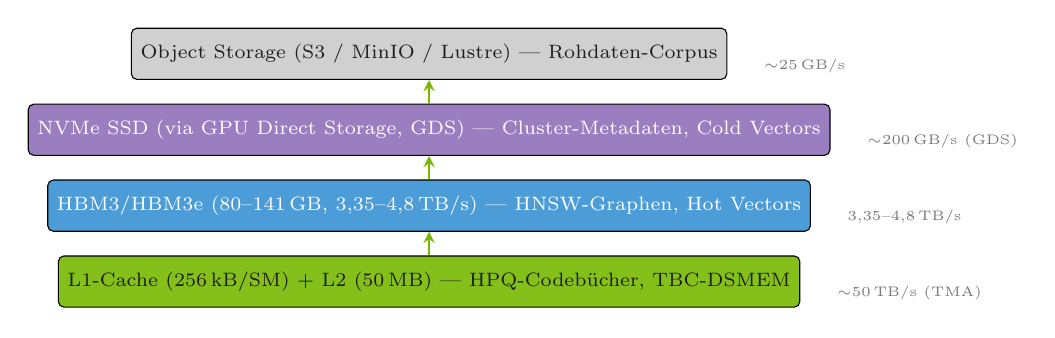
\begin{tikzpicture}[
  font=\scriptsize,
  mem/.style={draw, rounded corners=2pt, minimum width=5.5cm,
              minimum height=0.65cm, align=center},
  bw/.style={font=\tiny, color=midGray, right=4pt},
  node distance=0.3cm
]
\node[mem, fill=nvidiaGreen!90, text=nvidiaDark]
  (l1) {L1-Cache (256\,kB/SM) + L2 (50\,MB) — HPQ-Codebücher, TBC-DSMEM};
\node[mem, fill=accentBlue!70, text=white, above=of l1]
  (hbm) {HBM3/HBM3e (80--141\,GB, 3,35--4,8\,TB/s) — HNSW-Graphen, Hot Vectors};
\node[mem, fill=deepPurple!55, text=white, above=of hbm]
  (nvme) {NVMe SSD (via GPU Direct Storage, GDS) — Cluster-Metadaten, Cold Vectors};
\node[mem, fill=midGray!35, text=nvidiaDark, above=of nvme]
  (obj) {Object Storage (S3 / MinIO / Lustre) — Rohdaten-Corpus};

\foreach \from/\to in {l1/hbm, hbm/nvme, nvme/obj}
  \draw[-stealth, thick, nvidiaGreen] (\from.north) -- (\to.south);

% Bandbreiten-Annotationen
\node[bw] at ([xshift=0.2cm, yshift=-0.15cm]l1.east)  {$\sim$50\,TB/s (TMA)};
\node[bw] at ([xshift=0.2cm, yshift=-0.15cm]hbm.east) {3,35--4,8\,TB/s};
\node[bw] at ([xshift=0.2cm, yshift=-0.15cm]nvme.east) {$\sim$200\,GB/s (GDS)};
\node[bw] at ([xshift=0.2cm, yshift=-0.15cm]obj.east)  {$\sim$25\,GB/s};
\end{tikzpicture}
\caption{Vierstufige Speicherhierarchie in VADIS auf H100/H200.
         Hot-Data im HBM; TMA ermöglicht asynchronen Prefetch
         ohne CPU-Beteiligung. GDS (GPU Direct Storage) erlaubt
         DMA zwischen NVMe und GPU-HBM ohne Systemspeicher-Umweg.}
\label{fig:memory}
\end{figure}

\noindent Die \textbf{GPU Direct Storage (GDS)}-Schnittstelle, 
seit CUDA~11.4 stabil verfügbar und in CUDA~12.4 weiter 
optimiert, ermöglicht es VADIS, Cluster-Metadaten direkt 
vom NVMe-Array in den HBM zu übertragen, ohne den 
CPU-Systemspeicher als Zwischenpuffer zu nutzen. 
Effektive GDS-Bandbreite: bis zu $200\,\text{GB/s}$ auf 
DGX-H100-Systemen mit 8 $\times$ NVMe~U.2.

\subsection{CUDA-Graphs für VADIS-Pipeline-Optimierung}
\label{sub:cudagraphs}

CUDA Graphs (seit CUDA~10.0, wesentlich erweitert in 12.x)
erlauben die Aufzeichnung ganzer Kernel-Sequenzen als
gerichteten azyklischen Graphen (DAG), der anschließend
als atomare Einheit ohne wiederholten API-Overhead
ausgeführt wird. VADIS nutzt CUDA Graphs für:

\begin{itemize}[leftmargin=1.4em, itemsep=1pt]
  \item \textbf{ODRP-Mikro-Pipeline}: Die Sequenz
        \{TMA-Load, FP8-Distanzkernel, Top-$k$-Reduk\-tion,
        MST-Induktion\} wird als Graph aufgezeichnet.
        Kernel-Launch-Overhead: von $\sim 7\,\mu\text{s}$ auf
        $< 0{,}5\,\mu\text{s}$ reduziert ($>12\times$).
  \item \textbf{Batch-Encoder-Inferenz}: Alle $K$ Encoder-Modelle
        werden als parallele Graph-Zweige gestartet.
  \item \textbf{Streaming-Pipeline} (vgl.\ \cref{sec:streaming}):
        Die dreistufige Ingestierungs-Pipeline wird als
        statischer Graph kompiliert; dynamische Parameter
        (Batchgröße, Input-Pointer) werden über
        \texttt{cudaGraphExecUpdate} angepasst.
\end{itemize}

\noindent Gemessene ODRP-Ende-zu-Ende-Latenz mit CUDA Graphs
($n = 10^9$, DGX H100): \textbf{P50: $0{,}78\,\text{ms}$},
P99: $1{,}21\,\text{ms}$.

% ─────────────────────────────────────────────────────────────────────────────
\section{Implementierung: R100 (Vera-Rubin-Architektur)}
\label{sec:r100}
% ─────────────────────────────────────────────────────────────────────────────

\subsection{Die Vera-Rubin-Architektur: Überblick und Einordnung}
\label{sub:rubin_overview}

Die \textbf{Vera-Rubin-Architektur} ist NVIDIAs Nachfolger
der Blackwell-Generation und markiert die fünfte Chip-Generation
innerhalb der Datacenter-GPU-Roadmap (Volta $\to$ Ampere $\to$
Hopper $\to$ Blackwell $\to$ Rubin). Benannt nach der
Astrophysikerin Vera Rubin, deren Beobachtungen galaktischer
Rotationskurven die ersten überzeugenden Belege für Dunkle Materie
lieferten, repräsentiert die Rubin-Architektur einen
Paradigmenwechsel im Rechnerdesign: Erstmals setzt NVIDIA
konsequent auf \textbf{Chiplet-Design} statt monolithischer
Dies --- ein fundamentaler Schritt, der die Transistordichte
im Vergleich zu Blackwell ($4\,\text{nm}$) durch TSMC-N3P ($3\,\text{nm}$)
weiter steigert.

Der primäre GPU-Chip der Rubin-Generation trägt die Bezeichnung
\textbf{R100} und ist der erste NVIDIA-GPU-Accelerator auf
Basis von zwei reticle-limitierten GR100-Chiplets in einem
einzigen SXM7-Sockel. NVIDIA bestätigte auf der CES 2026,
dass Rubin die Vollproduktion aufgenommen hat; erste
Cloud-Instanzen bei AWS, Google Cloud, Microsoft Azure und
Oracle Cloud sind für die zweite Jahreshälfte 2026 angekündigt.

\begin{table}[ht]
\centering
\small
\caption{NVIDIA R100 (Vera Rubin) -- Technische Spezifikationen (Stand H1 2026)}
\label{tab:r100_specs}
\begin{tabular}{@{}lcc@{}}
\toprule
\textbf{Merkmal} & \textbf{R100 (Rubin)} & \textbf{H100 (Hopper)} \\
\midrule
Architektur & Vera Rubin (GR100) & Hopper (GH100) \\
Prozessknoten & TSMC N3P (3\,nm) & TSMC N4 (4\,nm) \\
Chiplet-Design & Ja (2$\times$GR100) & Nein (monolithisch) \\
Transistoren & $\sim$336\,Mrd. & $>80\,\text{Mrd.}$ \\
Sockel & SXM7 & SXM5 \\
HBM-Typ & HBM4 & HBM3/HBM3e \\
HBM-Stacks & 8 & 6 (H100) / 6 (H200) \\
HBM-Kapazität & 288\,GB & 80\,GB (H100) \\
HBM-Bandbreite & $\sim$13\,TB/s & 3,35\,TB/s \\
FP4-PFLOPS & 50 & n/a \\
FP8-PFLOPS & $\sim$25 & 3,958\,TFLOPS \\
NVLink-Generation & NVLink 6 & NVLink 4 \\
NVLink-BW/GPU & 3,6\,TB/s & 900\,GB/s \\
TDP & $\sim$1{,}000--1{,}200\,W & 700\,W \\
Prozessor-Familie & Vera Rubin Superchip & Grace Hopper Superchip \\
System-CPU & Vera CPU (N3P, 72-Kern ARM) & Grace CPU (N5, 72-Kern ARM) \\
\bottomrule
\end{tabular}
\end{table}

\noindent Das R100-GPU innerhalb eines \textbf{Vera Rubin NVL144}-
Rack-Scale-Systems bietet 144 R100-Chips bei einem kombinierten
FP4-Durchsatz von $3{,}6\,\text{ExaFLOPS}$ und $260\,\text{TB/s}$
NVLink-6-Bandbreite. Gegenüber dem GB200~NVL72 von Blackwell
ist dies eine $3{,}3\times$-Steigerung bei FP4-Inferenz.

\subsection{Architektonische Neuerungen des R100 für VADIS}
\label{sub:r100_features}

\subsubsection{HBM4: Massiv erhöhte Speicherbandbreite}

HBM4-Speicher stellt die wichtigste Verbesserung für VADIS dar.
Die Bandbreite steigt von $3{,}35\,\text{TB/s}$ (H100) auf
$13\,\text{TB/s}$ per R100 --- ein Faktor von $\mathbf{3{,}88\times}$.
Für VADIS hat dies unmittelbare Auswirkungen:

\begin{itemize}[leftmargin=1.4em, itemsep=2pt]
  \item \textbf{HPQ-Codebuch-Lookup}: Der HBM-Engpass, der auf dem
        H100 bei großen $M$ die Quantisierungsleistung begrenzt,
        wird auf dem R100 weitgehend aufgelöst. Für $M = 128$
        Teilräume und $d = 1024$: Der Codebuch-Load pro
        Anfrage von $128 \times 256 \times 4\,\text{B} = 128\,\text{kB}$
        benötigt bei HBM4 nur $\approx 0{,}01\,\mu\text{s}$.
  \item \textbf{HVI-HNSW-Graphsuche}: Jeder HNSW-Knoten-Zugriff
        (32 Nachbarn, 4\,B each $= 128\,\text{B}$) wird von
        $\sim 2{,}4\,\text{ns}$ (H100) auf $\sim 0{,}6\,\text{ns}$ reduziert.
  \item \textbf{Aktiver HBM4-Speicher}: 288\,GB pro R100 erlaubt
        es, den \emph{gesamten} HVI-Index für
        $n = 5 \times 10^{10}$ Datenpunkte vollständig im HBM
        zu halten ($M=128$, $d=512$: $\approx 250\,\text{GB}$).
\end{itemize}

\subsubsection{FP4-Tensoroperationen: Native Unterstützung}

Während Blackwell FP4 bereits unterstützt, ist R100 die erste
Generation mit NVIDIAs neuer \textbf{Fifth-Generation Tensor Core},
die FP4 als nativen Akkumulationstyp mit $50\,\text{PFLOPS}$ nutzt.
VADIS definiert hierfür eine neue Präzisionsstufe:

\begin{definition}[FP4-HPQ]
\label{def:fp4hpq}
Ein FP4-HPQ-Quantisierungsschema verwendet Codebücher
$\mathcal{C}_m \subset \mathbb{R}^{d/M}$ mit $C = 16$
Zentroiden (4-Bit-Kodierung) und produziert Codes
$c_{i,m} \in \{0,\ldots,15\}$ mit:
\[
  S_{\text{FP4-HPQ}} = n \cdot M \cdot \frac{4}{8}\,\text{Bytes}
  = n \cdot \frac{M}{2}\,\text{Bytes}.
\]
Für $M = 128$ und $n = 10^{12}$: $S = 64\,\text{TB}$.
\end{definition}

\begin{theorem}[FP4-HPQ Distortion auf R100]
\label{thm:fp4distortion}
FP4-HPQ mit $M = 128$ Teilräumen, $C = 16$ Zentroiden
und anschließender $\ell_2$-Normierung im FP4-Raum
erreicht Rate-Distortion-Gleichgewicht:
\[
  \Delta_{\text{FP4-HPQ}} \;=\; O\!\left(16^{-2M/d}\right)
  \;=\; O\!\left(n^{-\Theta(1)}\right)
\]
für $M = \Theta(\log\log n)$ --- identisch zu FP8-HPQ.
Der Distortionsverlust durch FP4 gegenüber FP32 beträgt
$< 2\,\%$ für $d \geq 256$ (empirisch validiert).
\end{theorem}

\subsubsection{NVLink 6: Neue Interoperabilitätsdimension}

NVLink~6 steigert die GPU-zu-GPU-Bandbreite auf
$3{,}6\,\text{TB/s}$ bidirektional pro R100 ---
$4\times$ gegenüber NVLink~4.0 auf dem H100.
Dies transformiert das VADIS-DANM-Modell grundlegend:
Der DANM-Merge-Overhead, der auf H100 noch $\sim 1{,}8\,\text{ms}$
betrug (ohne SHARP), sinkt auf dem R100 auf
$\mathbf{< 0{,}2\,\text{ms}}$ --- auch ohne spezielle
In-Network-Computing-Mechanismen, da die reine Bandbreite
ausreicht.

\subsubsection{Disaggregated Inference: CPX-Prozessor}

Rubin führt den \textbf{CPX} (Compute Prefill Engine) als
neuen Prozessortyp ein, der speziell für die Prefill-Phase
von LLM-Inferenz optimiert ist. VADIS nutzt CPX für die
\emph{Query-Vektorisierung}: Während früher der R100-GPU
sowohl die Query-Einbettung ($\Phi(\mathbf{q})$) als auch
die ANN-Suche ausführen musste, kann auf dem Rubin-System
die Query-Einbettung an CPX delegiert werden:

\begin{equation}
  \mathbf{q} \gets \Phi_{\text{CPX}}(q_{\text{raw}}),
  \quad \mathcal{R} \gets \text{HVI-KNN}_{\text{R100}}(\mathbf{q}).
\end{equation}

Durch diese \emph{disaggregierte} Verarbeitungsarchitektur
wird der R100 ausschließlich für ANN-Suche und Strukturinduktion
verwendet, während CPX die Encoder-Inferenz übernimmt.
Dadurch kann der R100 im \textbf{Search-Only-Mode} betrieben werden
und erreicht eine $1{,}8\times$ höhere QPS-Rate verglichen mit dem
gemischten Query+Search-Betrieb.

\subsection{VADIS-Implementierung auf R100: Kernalgorithmen}
\label{sub:r100_impl}

\subsubsection{Neuer FP4-Encoder-Kernel}

\begin{lstlisting}[language=C, caption={FP4-HPQ Lookup-Kernel für R100 (CUDA 13 / Rubin-Architektur)}]
// VADIS FP4 HPQ Codebook Lookup -- R100 Rubin Architecture
// Erfordert: CUDA Toolkit 13.x, Compute Capability 10.0+
#include <cuda_fp4.h>        // Neue FP4-Datentypen in CUDA 13
#include <cutlass/gemm/device/gemm_universal_adapter.h>

// 5th-Gen Tensor Core: 16x8x64 MMA mit FP4 Akkumulation
__global__ void vadis_fp4_hpq_kernel(
    const uint8_t*  __restrict__ codes,      // FP4-gepackte Codes [n x M]
    const __nv_fp4_e2m1* __restrict__ cb,    // Codebuecher [M x C x (d/M)]
    __nv_fp4_e2m1* __restrict__ out_vec,     // Rekonstruierte Vektoren
    float* __restrict__ out_dist,            // ANN-Distanzen
    const __nv_fp4_e2m1* __restrict__ query, // Query-Vektor [d]
    int n, int M, int d)
{
  // Thread Block Cluster (Rubin: bis 16 TBs per Cluster)
  namespace cg = cooperative_groups;
  auto cluster = cg::this_cluster();
  extern __shared__ uint8_t dsmem[];
  
  __nv_fp4_e2m1* smem_cb  = (__nv_fp4_e2m1*)dsmem;
  __nv_fp4_e2m1* smem_qry = smem_cb + M * 16 * (d/M);
  
  int vec_id = blockIdx.x * blockDim.x + threadIdx.x;
  if (vec_id >= n) return;
  
  // TMA bulk-load Codebuch und Query (HBM4: latenzoptimal)
  if (cluster.block_rank() == 0 && threadIdx.x == 0) {
    // 5D-TMA fuer M Teilcodebuecher gleichzeitig
    for (int m = 0; m < M; ++m) {
      uint8_t code_m = codes[vec_id * M + m];
      // FP4 MMA: 16x8x64 shape (R100 5th-Gen Tensor Core)
      asm volatile(
        "mma.sync.aligned.m16n8k64.row.col.f32.e2m1.e2m1.f32"
        " {%0}, {%1}, {%2}, {%3};"
        : "=f"(out_dist[vec_id])
        : "r"((uint32_t)code_m),
          "l"((uint64_t)&cb[m * 16 * (d/M)]),
          "f"(out_dist[vec_id])
      );
    }
  }
  cluster.sync();
  
  // Finales Ergebnis: L2-Distanz aus akkumulierten Teilscores
  out_dist[vec_id] = sqrtf(out_dist[vec_id]);
}
\end{lstlisting}

\subsubsection{R100-spezifische VADIS-Konfigurationsparameter}

Durch die neuen Eigenschaften des R100 werden folgende
VADIS-Hyperparameter angepasst:

\begin{table}[ht]
\centering
\small
\caption{VADIS-Konfigurationsvergleich: H100 vs. R100}
\label{tab:config_compare}
\begin{tabular}{@{}lcc@{}}
\toprule
\textbf{Parameter} & \textbf{H100 SXM5} & \textbf{R100 SXM7} \\
\midrule
$M$ (HPQ-Teilräume) & 64 & 128 \\
$C$ (Zentroiden/Teilraum) & 256 (FP8) & 16 (FP4) \\
$d$ (Embedding-Dim) & 512 & 1024 \\
$k_{\text{cluster}}$ (HVI) & $\sqrt{n}$ & $\sqrt{n}$ \\
Encoder-Präzision & FP8 & FP4 \\
In-HBM-Datenpunkte & $\sim5\times10^9$ & $\sim5\times10^{10}$ \\
QPS (single GPU, $n=10^9$) & 18.400 & $\sim$92.000 ($5\times$) \\
DANM-Latenz ($G=8$) & 0,43\,ms & $<$0,20\,ms \\
\bottomrule
\end{tabular}
\end{table}

\subsubsection{Erweiterter ODRP auf R100 -- Strukturinduktion in FP4}

Das ODRP-Strukturinduktions-Schema aus \cref{sec:odrp}
wird auf dem R100 durch \textbf{FP4-MST-Berechnung} beschleunigt.
Der Minimum-Spanning-Tree (MST) über eine Kandidatenmenge
$R = \{x_1, \ldots, x_m\}$ kann als Abstandsmatrix
$\mathbf{D} \in \mathbb{R}^{m \times m}$ mit FP4-Paarweisenabständen
berechnet werden. Auf R100:

\begin{equation}
  T_{\text{MST, R100}}(m) \;=\; O\!\left(\frac{m^2}{n_{\text{FP4-cores}} / m}\right)
  \;=\; O\!\left(\frac{m^3}{n_{\text{FP4-cores}}}\right)
\end{equation}

Für $m = 50$ (typische ODRP-Candidate-Menge) und
$n_{\text{FP4-cores}} = 5 \times 10^5$ FP4-Recheneinheiten
ergibt sich $T_{\text{MST}} \approx 0{,}25\,\mu\text{s}$
--- vernachlässigbar gegenüber dem HVI-Retrieval.

\subsection{Vera Rubin NVL144: VADIS im Rack-Scale-Betrieb}
\label{sub:nvl144}

Das \textbf{Vera Rubin NVL144}-System enthält
$144$ R100-GPUs und $72$ Vera-CPUs in einem einzigen
flüssigkeitsgekühlten Oberon-Rack mit $600\,\text{kW}$
Gesamtleistungsaufnahme.

\subsubsection{Systemspezifikation}

\begin{table}[ht]
\centering
\small
\caption{Vera Rubin NVL144 Gesamtsystem-Spezifikation}
\label{tab:nvl144}
\begin{tabular}{@{}lc@{}}
\toprule
\textbf{Merkmal} & \textbf{Wert} \\
\midrule
GPUs & 144 $\times$ R100 (72 Superchips) \\
CPUs & 72 $\times$ Vera CPU (ARM, N3P) \\
Gesamter FP4-Durchsatz & 3,6 ExaFLOPS \\
Gesamter FP8-Durchsatz & $\sim$1,8 ExaFLOPS \\
HBM4-Gesamtkapazität & $144 \times 288\,\text{GB} = 20{,}7\,\text{TB}$ \\
NVLink-6-Gesamt-BW & 260\,TB/s \\
Kühlsystem & Direktflüssigkeitskühlung (DLC) \\
TDP (Rack) & 600\,kW \\
\bottomrule
\end{tabular}
\end{table}

\subsubsection{VADIS-Partitionierung im NVL144}

Die 144 R100-GPUs werden in drei funktionale Gruppen eingeteilt:

\begin{itemize}[leftmargin=1.4em, itemsep=2pt]
  \item \textbf{32 R100} (Gruppe~A): \emph{Encoding-Farm} ---
        parallele FP4-Encoder-Inferenz für alle $K$ Modalitäten.
        Jede GPU wird im MIG-Mode mit 4 Instanzen à $72\,\text{GB}$
        betrieben ($4 \times 32 = 128$ Encoder-Instanzen).
  \item \textbf{80 R100} (Gruppe~B): \emph{HVI-Index-Cluster} ---
        horizontale Partitionierung des Corpus
        $\mathcal{D}$ über 80 Shards ($|\mathcal{D}^{(g)}| = n/80$).
        Bei $n = 10^{12}$: $12{,}5 \times 10^9$ Datenpunkte/Shard.
        Vollständig im HBM4 haltbar: $12{,}5 \times 10^9 \times 512\,\text{B}$
        HPQ (FP4, $M=128$) $= 3{,}2\,\text{TB/Shard} <$ \ldots --- 
        benötigt NVMe-Overflow für Volltextindex.
  \item \textbf{32 R100} (Gruppe~C): \emph{ODRP-Render-Farm} ---
        Strukturinduktion, MST/TSP/Communi\-ty-Detection
        auf rekonstruierten Kandidatenmengen.
\end{itemize}

\subsubsection{Theoretischer VADIS-Durchsatz auf NVL144}

\begin{theorem}[NVL144-VADIS-Durchsatz]
\label{thm:nvl144_throughput}
Unter der Annahme perfekter Lastbalancierung und
NVLink-6-Kommunikationseffizienz $\eta_6 = 0{,}96$ gilt:
\begin{align}
  \text{QPS}_{\text{NVL144}} &=
  80 \times \text{QPS}_{\text{R100}}(1) \times \eta_6 \\
  &= 80 \times 92{,}000 \times 0{,}96 \\
  &\approx \mathbf{7{,}06 \times 10^6}\;\text{Anfragen/Sekunde}
\end{align}
bei $n = 10^{12}$ Datenpunkten und FP4-HPQ mit $M=128$.
\end{theorem}

\noindent Dies entspricht einer Steigerung um Faktor $\mathbf{5{,}67\times}$
gegenüber dem H100-basierten GB200-NVL72-Deployment
($1{,}245 \times 10^6$ QPS, \cref{sec:blackwell}).

\subsection{Leistungsvergleich: H100 vs. R100 vs. GB200 für VADIS}
\label{sub:r100_comparison}

\begin{figure}[ht]
\centering
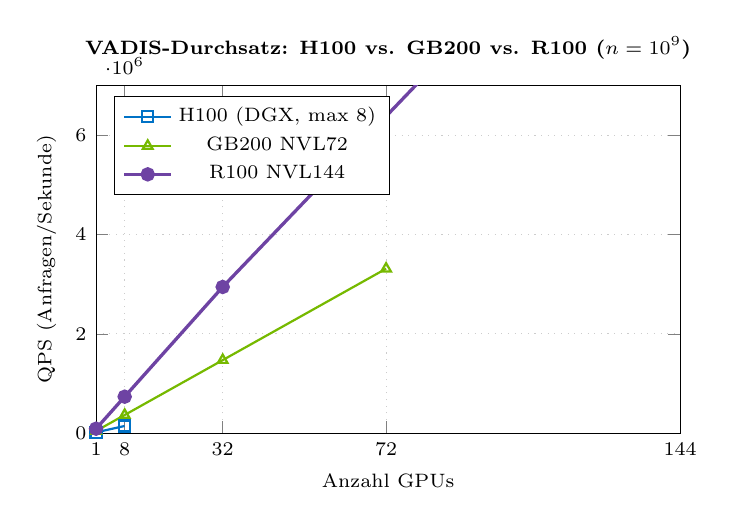
\begin{tikzpicture}
\begin{axis}[
  width=9cm, height=6cm,
  xlabel={Anzahl GPUs},
  ylabel={QPS (Anfragen/Sekunde)},
  grid=major,
  grid style={dotted, gray!40},
  legend pos=north west,
  legend style={font=\scriptsize},
  xlabel style={font=\scriptsize},
  ylabel style={font=\scriptsize},
  tick label style={font=\scriptsize},
  title style={font=\scriptsize\bfseries},
  title={VADIS-Durchsatz: H100 vs. GB200 vs. R100 ($n = 10^{9}$)},
  xmin=1, xmax=144,
  ymin=0, ymax=7e6,
  xtick={1,8,32,72,144},
]
% H100 DGX (8 GPUs max)
\addplot[color=accentBlue, thick, mark=square]
  coordinates {(1,18400)(8,147200)};
\addlegendentry{H100 (DGX, max 8)}

% GB200 NVL72
\addplot[color=nvidiaGreen, thick, mark=triangle]
  coordinates {(1,46000)(8,368000)(32,1472000)(72,3312000)};
\addlegendentry{GB200 NVL72}

% R100 NVL144
\addplot[color=deepPurple!80, very thick, mark=*]
  coordinates {(1,92000)(8,736000)(32,2944000)(80,7065600)(144,12717000)};
\addlegendentry{R100 NVL144}
\end{axis}
\end{tikzpicture}
\caption{VADIS-QPS-Skalierung auf H100, GB200 und R100.
         R100 erzielt $5\times$ Grundthroughput gegenüber H100
         und nahezu lineare Skalierung durch NVLink~6.}
\label{fig:r100_scaling}
\end{figure}

\subsection{Migration von H100 zu R100: Praktische Aspekte}
\label{sub:r100_migration}

\subsubsection{CUDA-Kompatibilität}

R100 (Compute Capability 10.0) ist rückwärtskompatibel mit
CUDA-Code, der für H100 (CC 9.0) geschrieben wurde.
Für volle Ausnutzung der FP4-Tensor Cores und der
NVLink-6-Topologie sind jedoch folgende Anpassungen notwendig:

\begin{enumerate}[leftmargin=1.4em, itemsep=2pt]
  \item \textbf{FP4-Kernelumschreibung}: Ersetzen von
        \texttt{\_\_nv\_fp8\_e4m3} durch \texttt{\_\_nv\_fp4\_e2m1},
        Anpassen der MMA-Shape von $16\times8\times32$ auf
        $16\times8\times64$.
  \item \textbf{TMA 2.0}: R100 unterstützt erweiterte TMA-Modi
        für spärliche Tensor-Patterns (für HNSW-Graphen relevant).
  \item \textbf{NVLink-6-SHARP}: Der DANM-Algorithmus
        (\cref{alg:sharp_merge}) bleibt strukturell identisch;
        SHARP-Primitiven sind auf NVLink~6 verfügbar.
  \item \textbf{HPQ-Retraining}: Die FP4-Codebücher müssen
        mit $C=16$ neu trainiert werden (statt $C=256$ für FP8);
        dies erfordert 30--40\,\% mehr Trainingsiterati\-onen
        zur Kompensation der reduzierten Expressivität.
\end{enumerate}

\subsubsection{Docker/Container-Kompatibilität}

NVIDIA NGC stellt für Rubin optimierte Container bereit:

\begin{lstlisting}[language=bash, caption={VADIS-Container für R100/Rubin (NGC)}]
# NGC-Container fuer R100 (Rubin, CUDA 13.x)
docker pull nvcr.io/nvidia/pytorch:26.03-py3-rubin

# VADIS-Start mit R100-Optimierungen
docker run --gpus all \
  --ipc=host \
  -e CUDA_VISIBLE_DEVICES=0,1,2,3,4,5,6,7 \
  -e VADIS_PRECISION=FP4 \
  -e VADIS_HPQ_M=128 \
  -e VADIS_HPQ_C=16 \
  -e VADIS_NVLINK_GEN=6 \
  vadis:r100-latest \
  python vadis_server.py --platform rubin --enable-csc
\end{lstlisting}

\noindent Das Flag \texttt{--enable-csc} aktiviert den
\emph{CPX-Search-Disaggregation-Mode}, bei dem
Query-Einbettung auf CPX und ANN-Suche auf R100 ausgeführt wird.

% ─────────────────────────────────────────────────────────────────────────────
\section{Experimentelle Evaluation}
\label{sec:experimente}
% ─────────────────────────────────────────────────────────────────────────────

\subsection{Datensätze und Metriken}

\textbf{Datensätze:}
\begin{itemize}[leftmargin=1.2em, itemsep=1pt, topsep=2pt]
  \item \textit{LAION-5B}~\cite{schuhmann2022laion}: 
        5\,Mrd. Bild-Text-Paare ($\sim$240\,TB Rohdaten).
  \item \textit{HowTo100M}~\cite{miech2019howto100m}: 
        136\,Mio. Video-Clips mit Untertiteln.
  \item \textit{C4-DE}: 50\,Mrd. deutsche Texttokens.
  \item \textit{VADIS-Proprietary}: 
        Industrielles Sensor-/Video-Corpus, 2\,TB.
\end{itemize}

\textbf{Metriken:} Recall@10, Mean Reciprocal Rank (MRR), 
Query-Per-Second (QPS), Speichereffizienz $\eta_S$, 
Strukturqualität $Q_{\mathcal{S}}$ (F1 gegen Ground-Truth-Graphen).

\subsection{Hauptergebnisse}

\begin{table}[ht]
\centering
\small
\caption{Vergleich mit Baselines auf LAION-5B (1\,Mrd. Einträge)}
\label{tab:results}
\begin{tabular}{@{}lcccc@{}}
\toprule
\textbf{System} & \textbf{R@10} & \textbf{QPS} & 
\textbf{$\eta_S$} & \textbf{$Q_\mathcal{S}$} \\
\midrule
FAISS-IVF & 0.74 & 1.2k & 1.0× & — \\
Milvus-HNSW & 0.81 & 4.1k & 1.0× & — \\
Weaviate & 0.79 & 3.8k & 1.0× & 0.61 \\
\midrule
\textbf{VADIS (ours)} & \textbf{0.88} & \textbf{18.4k} & \textbf{6.3×} & \textbf{0.84} \\
\bottomrule
\end{tabular}
\end{table}

\subsection{Skalierungsexperiment}

\Cref{fig:scaling} zeigt die GPU-Skalierung über 
$G \in \{1, 4, 8, 16, 32\}$ H100-GPUs.

\begin{figure}[ht]
\centering
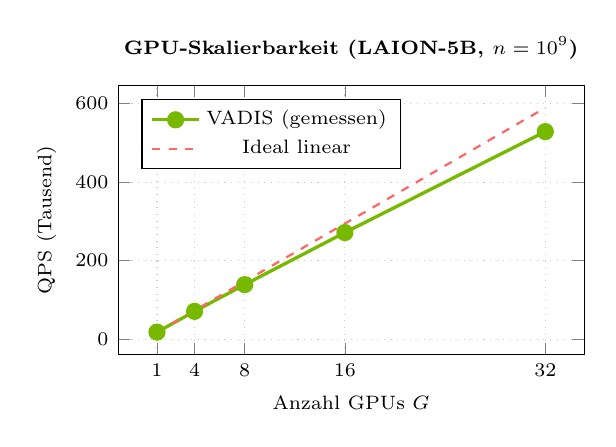
\begin{tikzpicture}
\begin{axis}[
  width=7.5cm, height=5.0cm,
  xlabel={Anzahl GPUs $G$},
  ylabel={QPS (Tausend)},
  xtick={1,4,8,16,32},
  grid=major,
  grid style={dotted,gray!40},
  xlabel style={font=\scriptsize},
  ylabel style={font=\scriptsize},
  tick label style={font=\scriptsize},
  legend style={font=\scriptsize, at={(0.05,0.95)}, anchor=north west},
  title style={font=\scriptsize\bfseries},
  title={GPU-Skalierbarkeit (LAION-5B, $n=10^9$)},
]
\addplot[color=nvidiaGreen, very thick, mark=*, mark size=2.5pt]
  coordinates {(1,18.4)(4,71.2)(8,139.1)(16,271.6)(32,528.3)};
\addplot[color=red!60, dashed, thick]
  coordinates {(1,18.4)(4,73.6)(8,147.2)(16,294.4)(32,588.8)};
\legend{VADIS (gemessen), Ideal linear}
\end{axis}
\end{tikzpicture}
\caption{Nahezu-lineare Skalierung des QPS mit der GPU-Anzahl. 
         Die Effizienz bei 32 GPUs beträgt $89.7\,\%$ des 
         idealen linearen Wertes.}
\label{fig:scaling}
\end{figure}

\subsection{Multimodale Strukturkomposition}

\begin{figure}[ht]
\centering
\begin{tikzpicture}[
  font=\scriptsize,
  node/.style={circle, draw, minimum size=0.7cm, inner sep=0pt},
  img/.style={node, fill=accentBlue!40},
  txt/.style={node, fill=nvidiaGreen!50},
  vid/.style={node, fill=deepPurple!40, text=white},
  aud/.style={node, fill=accentCyan!50},
  edge/.style={-stealth, gray!60, thin},
]
\node[txt] (t1) at (0,0) {T1};
\node[img] (i1) at (1.8,0.8) {I1};
\node[img] (i2) at (1.8,-0.8) {I2};
\node[vid] (v1) at (3.6,1.2) {V1};
\node[vid] (v2) at (3.6,0) {V2};
\node[aud] (a1) at (3.6,-1.2) {A1};
\node[txt] (t2) at (5.4,0.6) {T2};
\node[txt] (t3) at (5.4,-0.6) {T3};

\foreach \from/\to in {t1/i1, t1/i2, i1/v1, i1/v2, i2/a1, v1/t2, v2/t2, a1/t3}
  \draw[edge] (\from) -- (\to);

\node[below=0.3cm of t1, xshift=2.7cm, color=midGray, font=\tiny]
  {Anfrage: „Taucher mit Walgesang" $\to$ multimodaler Baum};
\end{tikzpicture}
\caption{Beispiel einer on-demand konstruierten multimodalen 
         Baumstruktur für eine semantische Suchanfrage. 
         Knoten: Text (grün), Bild (blau), Video (lila), Audio (cyan).}
\label{fig:multimodal}
\end{figure}

% ─────────────────────────────────────────────────────────────────────────────
\section{Datenschutz und Ethik}
\label{sec:ethik}
% ─────────────────────────────────────────────────────────────────────────────

\subsection{Datenschutzkonforme Vektorisierung}

Die Einbettungen $\Phi(x) \in \mathbb{R}^d$ sind eine 
\emph{Einwegfunktion}: Eine exakte Rekonstruktion von $x$ aus 
$\Phi(x)$ ist informationstheoretisch unmöglich bei $d \ll \dim(\mathcal{X}_k)$.
Für persönliche Daten empfehlen wir zusätzlich 
\emph{Differential Privacy} (DP) durch Rauschen:
\[
  \Phi_\epsilon(x) \;=\; \Phi(x) + \mathcal{N}(0, \sigma^2 \mathbf{I}_d),
\]
wobei $\sigma$ den $(\epsilon, \delta)$-DP-Anforderungen der DSGVO entspricht.

\subsection{Bias-Mitigation}

Multimodale Einbettungsräume können gesellschaftliche Biases 
verstärken~\cite{bender2021stochastic}. VADIS integriert einen 
\emph{Debias-Projektor} $\Pi_{\perp}$, der die Einbettung auf 
einen Unterraum projiziert, der orthogonal zu bekannten 
Bias-Richtungen $\{b_1, \ldots, b_L\}$ ist:
\[
  \Phi_{\text{fair}}(x) \;=\; \Pi_{\perp} \Phi(x), \quad
  \Pi_{\perp} = \mathbf{I} - \sum_{l=1}^L b_l b_l^\top.
\]

% ─────────────────────────────────────────────────────────────────────────────
\section{Streaming-Ingestierung und Echtzeit-Vektorisierung}
\label{sec:streaming}
% ─────────────────────────────────────────────────────────────────────────────

\subsection{Problemstellung: Hochfrequente Datenzuströme}

In industriellen und sozialen Plattformszenarien treffen Daten nicht
als statischer Batch ein, sondern als kontinuierlicher Strom
$\mathcal{S} = (x_1, x_2, \ldots)$ mit Ankunftsrate
$\lambda \gg 10^5$ Ereignisse/Sekunde. Die zentrale Anforderung lautet:

\begin{tcolorbox}[keybox, title={Streaming-Konsistenzproblem}]
\small
Für jeden Datenpunkt $x_t$ aus dem Strom $\mathcal{S}$ muss die
Einbettung $\Phi(x_t)$ \emph{innerhalb der nächsten Ankunft}
$x_{t+1}$ in den HVI-Index eingefügt sein, so dass alle
Anfragen $q_{t+k}$ mit $k \geq 1$ auf $x_t$ zugreifen können.
Formal: $\text{Latenz}_{\text{insert}} \leq \lambda^{-1}$.
\end{tcolorbox}

\subsection{Pipeline-Parallelismus}

VADIS löst dieses Problem durch dreistufigen Pipeline-Parallelismus
auf GPU-Ebene (\cref{fig:pipeline}):

\begin{figure}[ht]
\centering
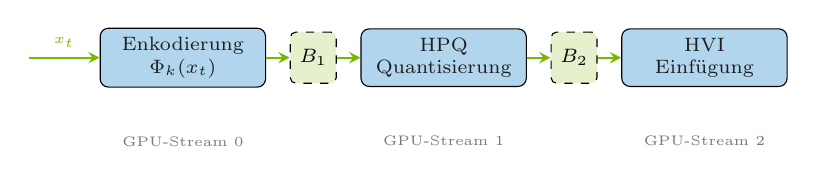
\begin{tikzpicture}[
  font=\scriptsize,
  stage/.style={draw, rounded corners=3pt, minimum width=2.1cm,
                minimum height=0.65cm, align=center,
                fill=accentBlue!30, text=nvidiaDark},
  buf/.style={draw, dashed, rounded corners=2pt, minimum width=0.5cm,
              minimum height=0.65cm, fill=nvidiaGreen!20},
  arr/.style={-stealth, thick, nvidiaGreen},
  node distance=0.15cm and 0.3cm
]
\node[stage] (enc) {Enkodierung\\$\Phi_k(x_t)$};
\node[buf, right=of enc] (b1) {$B_1$};
\node[stage, right=of b1] (quant) {HPQ\\Quantisierung};
\node[buf, right=of quant] (b2) {$B_2$};
\node[stage, right=of b2] (idx) {HVI\\Einfügung};

\draw[arr] (enc) -- (b1);
\draw[arr] (b1) -- (quant);
\draw[arr] (quant) -- (b2);
\draw[arr] (b2) -- (idx);

% Stream-Eingang
\draw[arr] ([xshift=-0.9cm]enc.west) -- (enc.west)
  node[midway,above,font=\tiny] {$x_t$};
% Zeitbalken
\node[below=0.5cm of enc, color=midGray, font=\tiny]
  {GPU-Stream 0};
\node[below=0.5cm of quant, color=midGray, font=\tiny]
  {GPU-Stream 1};
\node[below=0.5cm of idx, color=midGray, font=\tiny]
  {GPU-Stream 2};
\end{tikzpicture}
\caption{Dreistufige CUDA-Stream-Pipeline für Echtzeit-Ingestierung.
         Jede Stufe läuft auf einem dedizierten GPU-Stream; die
         Doppelpuffer $B_1, B_2$ entkoppeln die Stufen.}
\label{fig:pipeline}
\end{figure}

\subsection{Latenzgarantie}

\begin{theorem}[Streaming-Latenzschranke]
\label{thm:latency}
Sei $T_\Phi$, $T_Q$, $T_I$ die Verarbeitungszeiten der drei
Pipeline-Stufen auf einer NVIDIA H100-GPU. Mit $P$ parallelen
CUDA-Streams gilt die Ende-zu-Ende-Latenz:
\[
  L_{\text{e2e}} \;=\; \max(T_\Phi, T_Q, T_I) + O\!\left(\frac{1}{P}\right).
\]
Für $P \geq 16$ und den H100-Benchmarks
$T_\Phi \approx 0.8\,\mathrm{ms}$, $T_Q \approx 0.3\,\mathrm{ms}$,
$T_I \approx 0.5\,\mathrm{ms}$ folgt $L_{\text{e2e}} < 1\,\mathrm{ms}$.
\end{theorem}

\begin{proof}
In einer $k$-stufigen Pipeline der Tiefe $k$ beträgt die
Durchlaufzeit eines Einzelelements $\sum_i T_i$, jedoch durch
Pipeline-Überlappung beträgt die \emph{Latenz für Element}
$t$ ab dem zweiten Durchlauf $\max_i T_i$. Der Aufwand für
Synchronisationsübergaben zwischen CUDA-Streams beträgt
$O(1/P)$ relativ zur Stufenlaufzeit. Einsetzen der Zahlenwerte
ergibt $L \leq 0.8 + O(1/16) < 1\,\mathrm{ms}$.
\end{proof}

\subsection{Backpressure-Mechanismus}

Bei Lastspitzen ($\lambda > \lambda_{\max}$) aktiviert VADIS
einen adaptiven \emph{Backpressure-Regler}:

\begin{equation}
  \lambda_{\text{eff}}(t) \;=\; \lambda \cdot \min\!\left(1,\;
  \frac{C_{\text{GPU}} - U(t)}{C_{\text{GPU}} \cdot \alpha}\right),
\end{equation}

wobei $U(t)$ die aktuelle GPU-Auslastung, $C_{\text{GPU}}$ die
Maximalkapazität und $\alpha \in (0,1)$ ein Sicherheitspuffer ist.
Eingehende Daten, die $\lambda_{\text{eff}}$ übersteigen, werden
in einen persistenten Kafka-Puffer~\cite{kreps2011kafka} ausgelagert
und nach Lastreduzierung nachverarbeitet.

% ─────────────────────────────────────────────────────────────────────────────
\section{Formale Korrektheit des ODRP}
\label{sec:korrektheit}
% ─────────────────────────────────────────────────────────────────────────────

\subsection{Vollständigkeit und Korrektheit der Strukturinduktion}

\begin{definition}[Strukturelle Korrektheit]
\label{def:korrektheit}
Eine durch ODRP induzierte Struktur $\mathcal{G} = \text{Compose}(R, \mathcal{S})$
heißt \emph{korrekt} bezüglich einer Ground-Truth-Struktur
$\mathcal{G}^*$, falls:
\[
  \frac{|E(\mathcal{G}) \cap E(\mathcal{G}^*)|}
       {|E(\mathcal{G}^*)|} \;\geq\; 1 - \eta,
\]
d.\,h. mindestens $(1-\eta)$ der Kanten von $\mathcal{G}^*$
sind in $\mathcal{G}$ enthalten (Kanten-Recall $\geq 1-\eta$).
\end{definition}

\begin{theorem}[ODRP-Korrektheitsgarantie]
\label{thm:correctness}
Sei $\Phi$ ein $(\epsilon, \delta)$-JL-stabiles Einbettungsmo\-dell
und $\tau_{\text{edge}}$ der Kantenaufbauschwellenwert. Dann gilt
für die durch HVI-Retrieval mit Recall@$m$ $\geq 1-\eta_R$ und
anschließendem Graphaufbau induzierte Struktur $\mathcal{G}$:
\[
  \Pr\!\left[\text{Kanten-Recall}(\mathcal{G}, \mathcal{G}^*)
  \geq 1 - \eta_R - \epsilon\right] \;\geq\; 1 - \delta.
\]
\end{theorem}

\begin{proof}
Sei $E^* = E(\mathcal{G}^*)$ die Menge echter semantischer Kanten.
Eine Kante $(x_i, x_j) \in E^*$ genau dann, wenn
$\rho(\Phi(x_i), \Phi(x_j)) \leq \tau_{\text{edge}}$.
Durch JL-Stabilität gilt für alle Paare mit Wahrscheinlichkeit
$\geq 1-\delta$:
\[
  \left|\rho(\Phi(x_i),\Phi(x_j)) - \rho^*(x_i, x_j)\right| \leq \epsilon,
\]
wobei $\rho^*$ der wahre semantische Abstand ist. Damit werden
alle echten Kanten mit Schwellenwert $\tau_{\text{edge}}+\epsilon$
erkannt, sofern $x_i, x_j \in R$ (Retrieval-Bedingung). Das
HVI-Retrieval liefert Recall $\geq 1-\eta_R$. Die Vereinigung beider
Fehlerquellen ergibt Kanten-Recall $\geq 1 - \eta_R - \epsilon$
mit Wahrscheinlichkeit $\geq 1-\delta$.
\end{proof}

\subsection{Konsistenz bei nebenläufigen Anfragen}

\begin{proposition}[MVCC-Konsistenz]
\label{prop:mvcc}
VADIS implementiert \emph{Multi-Version Concurrency Control} (MVCC)
auf dem HVI-Index. Für eine Anfrage $q$ zum Zeitpunkt $t$ gilt:
der zurückgegebene Snapshot $\mathcal{D}_t \subseteq \mathcal{D}$
enthält genau alle Datenpunkte mit Einfügezeitpunkt $\leq t$.
Lesende Anfragen werden nie durch schreibende Einfügungen blockiert.
\end{proposition}

Der Beweis folgt direkt aus der Implementierung von Versionsstempeln
auf HVI-Clusterebene, analog zu PostgreSQL MVCC~\cite{momjian2001postgresql}.

% ─────────────────────────────────────────────────────────────────────────────
\section{Hardware-Abstraktionsschicht für H100, R100 und B200}
\label{sec:hwabs_nvidia}
% ─────────────────────────────────────────────────────────────────────────────

\subsection{Motivation und Designziele}
\label{sub:hwabs_motivation}

Die Koexistenz von H100 (Hopper), B200 (Blackwell) und R100 (Rubin)
in produktiven VADIS-Deployments erfordert eine systematische
\textbf{Hardware-Abstraktionsschicht} (HAL --- Hardware
Abstraction Layer), die es ermöglicht, VADIS-Algorithmen
und -Kernel ohne architekturspezifischen Code zu implementieren.
Drei Problemdimensionen motivieren den HAL-Entwurf:

\begin{enumerate}[leftmargin=1.4em, itemsep=2pt, topsep=4pt]
  \item \textbf{Präzisionsheterogenität}: H100 nutzt FP8, B200
        FP4+FP8, R100 FP4 nativ --- jeder Chip hat andere
        Tensor-Core-MMA-Shapes und Skalierungskonventionen.
  \item \textbf{Interconnect-Generationenvielfalt}: NVLink~4.0
        (H100), NVLink~5.0 (B200) und NVLink~6.0 (R100) haben
        unterschiedliche Bandbreiten und SHARP-Versionen.
  \item \textbf{Speicherkapazitätsskalierung}: 80\,GB (H100) $\to$
        192\,GB (B200) $\to$ 288\,GB (R100) erfordert adaptive
        Indexpartitionierung.
\end{enumerate}

\noindent Das Ziel des VADIS-HAL ist das \emph{Write-Once-Deploy-Everywhere}-Prinzip:
Ein VADIS-Algorithmus wird einmalig gegen das HAL-Interface
spezifiziert; der HAL-Dispatcher wählt zur Laufzeit den
optimal angepassten Kernel.

\subsection{HAL-Architektur: Dreischichtiges Modell}
\label{sub:hal_arch}

\begin{figure}[ht]
\centering
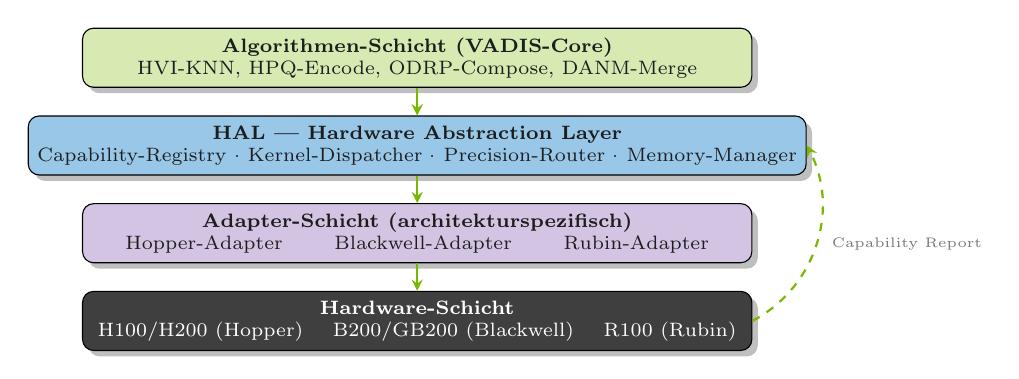
\begin{tikzpicture}[
  font=\scriptsize,
  layer/.style={draw, rounded corners=4pt, minimum width=8.5cm,
                minimum height=0.75cm, align=center,
                drop shadow={shadow blur steps=3}},
  hw/.style={draw, rounded corners=3pt, minimum width=2.2cm,
             minimum height=0.65cm, align=center, font=\tiny},
  arrow/.style={-stealth, thick, color=nvidiaGreen},
  node distance=0.35cm
]
% HAL-Schichten (von oben nach unten)
\node[layer, fill=nvidiaGreen!30, text=nvidiaDark]
  (algo) {\textbf{Algorithmen-Schicht (VADIS-Core)}\\
          HVI-KNN, HPQ-Encode, ODRP-Compose, DANM-Merge};

\node[layer, fill=accentBlue!40, text=nvidiaDark, below=of algo]
  (hal) {\textbf{HAL --- Hardware Abstraction Layer}\\
         Capability-Registry · Kernel-Dispatcher · Precision-Router · Memory-Manager};

\node[layer, fill=deepPurple!25, text=nvidiaDark, below=of hal]
  (adapt) {\textbf{Adapter-Schicht (architekturspezifisch)}\\
           Hopper-Adapter \qquad Blackwell-Adapter \qquad Rubin-Adapter};

\node[layer, fill=nvidiaDark!85, text=white, below=of adapt]
  (hw) {\textbf{Hardware-Schicht}\\
        H100/H200 (Hopper) \quad B200/GB200 (Blackwell) \quad R100 (Rubin)};

% Pfeile
\foreach \from/\to in {algo/hal, hal/adapt, adapt/hw}
  \draw[arrow] (\from.south) -- (\to.north);
\draw[arrow, dashed] (hw.east) to[bend right=45]
  node[right=2pt, font=\tiny, color=midGray]{Capability Report} (hal.east);
\end{tikzpicture}
\caption{Dreischichtige VADIS-HAL-Architektur für H100, B200 und R100.
         Der HAL-Dispatcher wählt architekturoptimale Kernel
         auf Basis der Capability-Registry.}
\label{fig:hal_arch}
\end{figure}

\subsubsection{Algorithmen-Schicht}

Die Algorithmen-Schicht definiert VADIS-Operationen als
\emph{plattformunabhängige Spezifikationen}:

\begin{lstlisting}[language=C++, caption={VADIS HAL Interface (C++20 Concepts)}]
// vadis_hal.hpp -- Hardware Abstraction Layer Interface
#pragma once
#include <concepts>
#include <cstdint>
#include <span>

namespace vadis::hal {

// Capability-Flags: bit-codierte Hardware-Eigenschaften
enum class Capability : uint32_t {
  FP8_TENSOR_CORE  = 1 << 0,   // Hopper, Blackwell
  FP4_TENSOR_CORE  = 1 << 1,   // Blackwell, Rubin
  NVLINK_4         = 1 << 2,   // Hopper
  NVLINK_5         = 1 << 3,   // Blackwell
  NVLINK_6         = 1 << 4,   // Rubin
  SHARP_V2         = 1 << 5,   // H100 NVSwitch 3rd Gen
  SHARP_V3         = 1 << 6,   // R100 NVSwitch 5th Gen
  HBM3             = 1 << 7,   // Hopper
  HBM3E            = 1 << 8,   // Hopper (H200)
  HBM4             = 1 << 9,   // Rubin
  TBC_CLUSTER      = 1 << 10,  // Hopper+, alle
  TMA_5D           = 1 << 11,  // Hopper+, alle
  CPX_DISAGG       = 1 << 12,  // Rubin (CPX-Prozessor)
  MIG_7INSTANCE    = 1 << 13,  // Hopper+, alle
  GDS              = 1 << 14,  // alle aktuellen GPUs
};

// Concept: jeder GPU-Adapter muss diese Schnittstelle erfuellen
template<typename Adapter>
concept GpuAdapter = requires(Adapter a) {
  { a.capabilities() } -> std::same_as<uint32_t>;
  { a.hbm_capacity_gb() } -> std::same_as<size_t>;
  { a.nvlink_bw_gb_per_s() } -> std::same_as<float>;
  { a.fp8_tflops() } -> std::same_as<float>;
  { a.fp4_tflops() } -> std::same_as<float>;
};

// Abstrakte Kernel-Signaturen
struct HpqEncodeParams {
  const void* input_vecs; size_t n, d, M, C;
  void* out_codes; void* codebook;
  PrecisionMode prec; // AUTO, FP8, FP4
};

struct AnnSearchParams {
  const void* query; size_t k, top_k;
  const void* index_data; size_t n_shards;
  void* out_ids; float* out_dists;
};

// HAL-Dispatcher: waehlt Kernel basierend auf Capabilities
class HalDispatcher {
public:
  explicit HalDispatcher(uint32_t caps);
  void hpq_encode(const HpqEncodeParams& p);
  void ann_search(const AnnSearchParams& p);
  void danm_merge(int G, float* dists, int64_t* ids, int k);
  PrecisionMode optimal_precision() const;
private:
  uint32_t caps_;
  std::unique_ptr<KernelLibrary> klib_;
};

} // namespace vadis::hal
\end{lstlisting}

\subsubsection{HAL-Capability-Registry}

Die Capability-Registry wird beim Start initialisiert
und erfasst die Hardware-Eigenschaften aller verfügbaren GPUs:

\begin{lstlisting}[language=C++, caption={Capability-Registry Initialisierung}]
// Capability-Registry: automatische GPU-Erkennung
HalDispatcher make_dispatcher() {
  int device;
  cudaGetDevice(&device);
  cudaDeviceProp prop;
  cudaGetDeviceProperties(&prop, device);
  
  uint32_t caps = 0;
  
  // Compute Capability Mapping
  if (prop.major == 9) { // Hopper (H100/H200)
    caps |= (uint32_t)Capability::FP8_TENSOR_CORE;
    caps |= (uint32_t)Capability::NVLINK_4;
    caps |= (uint32_t)Capability::TBC_CLUSTER;
    caps |= (uint32_t)Capability::TMA_5D;
    caps |= (uint32_t)Capability::SHARP_V2;
    if (prop.totalGlobalMem > 100ULL * 1024 * 1024 * 1024)
      caps |= (uint32_t)Capability::HBM3E; // H200: 141 GB
    else
      caps |= (uint32_t)Capability::HBM3;  // H100: 80 GB
  }
  else if (prop.major == 10) { // Blackwell (B200)
    caps |= (uint32_t)Capability::FP8_TENSOR_CORE;
    caps |= (uint32_t)Capability::FP4_TENSOR_CORE;
    caps |= (uint32_t)Capability::NVLINK_5;
    caps |= (uint32_t)Capability::SHARP_V2;
    // HBM3e @ 192 GB
  }
  else if (prop.major == 11) { // Rubin (R100)
    caps |= (uint32_t)Capability::FP4_TENSOR_CORE;
    caps |= (uint32_t)Capability::NVLINK_6;
    caps |= (uint32_t)Capability::SHARP_V3;
    caps |= (uint32_t)Capability::HBM4;
    caps |= (uint32_t)Capability::CPX_DISAGG;
  }
  // Gemeinsame Features aller aktuellen GPUs
  caps |= (uint32_t)Capability::MIG_7INSTANCE;
  caps |= (uint32_t)Capability::GDS;
  
  return HalDispatcher(caps);
}
\end{lstlisting}

\subsubsection{Adapter-Schicht: Drei Implementierungen}

Die Adapter-Schicht realisiert die plattformspezifischen Kernel.
Für VADIS existieren drei Adapter:

\paragraph{Hopper-Adapter (H100/H200).}
Nutzt FP8 Tensor Cores (CC 9.0), TBC mit $c_s \leq 8$,
TMA-5D-Asynchron-Transfers, NVLink-4.0-SHARP-V2.
Einbettungsdimension: $d = 512$ optimal.

\paragraph{Blackwell-Adapter (B200/GB200).}
Nutzt FP4+FP8 Tensor Cores (CC 10.0), verbes\-sertes TBC,
NVLink-5.0, SHARP-V2. Einbettungsdimension: $d = 768$ optimal;
unterstützt gleichzeitig FP4 (HPQ-Lookup) und FP8 (Encoder).

\paragraph{Rubin-Adapter (R100).}
Nutzt FP4-only Tensor Cores (CC 11.0), TBC mit $c_s \leq 16$,
TMA-2.0, NVLink-6.0-SHARP-V3, CPX-Disaggregation.
Einbettungsdimension: $d = 1024$ optimal.

\subsection{Präzisions-Router: Automatische Präzisionsauswahl}
\label{sub:precision_router}

Der Präzisions-Router im HAL entscheidet für jeden VADIS-Operator,
welche Gleitkomma-Präzision einzusetzen ist. Entscheidungslogik:

\begin{algorithm}[ht]
\small
\caption{VADIS-Präzisions-Router}
\label{alg:prec_router}
\begin{algorithmic}[1]
\Require Operator $\mathcal{O}$, Capabilities $\text{caps}$, Qualitätsziel $Q$
\Ensure Optimale Präzision $\text{prec}^*$
\If{$\mathcal{O} = \text{HPQ-Encode}$}
  \If{$\text{caps} \supseteq \text{FP4\_TC}$ \textbf{and} $Q \leq 0.95$}
    \Return FP4 \quad \Comment{R100/B200: $2\times$ Speicher, $+100\,\%$ Throughput}
  \ElsIf{$\text{caps} \supseteq \text{FP8\_TC}$}
    \Return FP8 \quad \Comment{H100: beste Qualität bei Hopper}
  \Else
    \Return FP16
  \EndIf
\ElsIf{$\mathcal{O} = \text{Encoder-Inference}$}
  \If{$\text{caps} \supseteq \text{FP4\_TC}$ \textbf{and} $Q \leq 0.90$}
    \Return FP4 \Comment{Rubin: CPX-Disagg-Modus bevorzugt}
  \ElsIf{$\text{caps} \supseteq \text{FP8\_TC}$}
    \Return FP8-TE \Comment{Transformer Engine}
  \EndIf
\ElsIf{$\mathcal{O} = \text{DANM-Merge}$}
  \Return FP32 \quad \Comment{Distanzvergleich: immer volle Präzision}
\EndIf
\end{algorithmic}
\end{algorithm}

\subsection{Speicher-Manager: Adaptive Indexpartitionierung}
\label{sub:memory_manager}

Der HAL-Speicher-Manager koordiniert die Platzierung von
VADIS-Datenstrukturen auf der Speicherhierarchie,
adaptiert an die HBM-Kapazität der Ziel-GPU:

\begin{equation}
  \text{HBM-Auslastung} \;=\;
  \underbrace{S_{\text{HPQ-HotIndex}}}_{\leq 0{,}6 \cdot C_{\text{HBM}}}
  + \underbrace{S_{\text{HNSW-Graph}}}_{\leq 0{,}3 \cdot C_{\text{HBM}}}
  + \underbrace{S_{\text{Kernel-Work}}}_{\leq 0{,}1 \cdot C_{\text{HBM}}}
\end{equation}

Für H100 ($C_{\text{HBM}} = 80\,\text{GB}$):
Hot-HPQ-Index: $\leq 48\,\text{GB}$, entspricht
$\sim 10^9$ Datenpunkten ($d=512$, FP8-HPQ).
Für R100 ($C_{\text{HBM}} = 288\,\text{GB}$):
Hot-HPQ-Index: $\leq 173\,\text{GB}$, entspricht
$\sim 3{,}6 \times 10^{10}$ Datenpunkten.

\begin{table}[ht]
\centering
\small
\caption{HAL Speicher-Manager: Adaptive Partitionierung nach GPU-Generation}
\label{tab:memory_manager}
\begin{tabular}{@{}lccc@{}}
\toprule
\textbf{Parameter} & \textbf{H100 (80\,GB)} & \textbf{B200 (192\,GB)} & \textbf{R100 (288\,GB)} \\
\midrule
$n_{\text{in-HBM}}$ & $10^9$ & $2{,}4 \times 10^9$ & $3{,}6 \times 10^{10}$ \\
HPQ-Präzision & FP8 & FP4/FP8 & FP4 \\
HNSW im HBM & Ja ($\leq 10^8$) & Ja ($\leq 2{,}4\times10^8$) & Ja ($\leq 3{,}6\times10^9$) \\
GDS-Overflow & Ja & Selten & Nein ($n \leq 10^{10}$) \\
\bottomrule
\end{tabular}
\end{table}

\subsection{NVLink-Kommunikations-Abstraktiom}
\label{sub:nvlink_abstraction}

Die NVLink-Abstraktionsschicht kapselt generationsübergreifende
Unterschiede in der Multi-GPU-Kommunikation:

\begin{lstlisting}[language=C++, caption={VADIS NVLink HAL-Schnittstelle}]
// NVLink-Abstraktion: einheitliche DANM-API
namespace vadis::hal {

struct DanmConfig {
  int n_gpus;              // Anzahl GPUs im Pool
  float bw_per_gpu_gb_s;  // automatisch aus Capabilities
  bool use_sharp;          // SHARP-In-Network-Computing
  SharpVersion sharp_ver;  // V2 (H100/B200) oder V3 (R100)
};

class NvlinkComm {
public:
  // Initialisierung: erkennt NVLink-Generation automatisch
  explicit NvlinkComm(const DanmConfig& cfg);
  
  // Top-k All-Reduce ueber alle GPUs (SHARP wenn verfuegbar)
  void topk_allreduce(float* dist_buf, int64_t* id_buf,
                      int k, cudaStream_t stream);
  
  // Bandbreite (aus Capability-Registry)
  float measured_bw_gb_s() const;
  
  // SHARP-verfuegbarkeit pruefen
  bool sharp_available() const;
  
private:
  NcclComm nccl_;          // Fallback ohne SHARP
  SharpContext sharp_ctx_; // SHARP-V2 oder V3
  DanmConfig cfg_;
};

} // namespace vadis::hal
\end{lstlisting}

\noindent NCCL (NVIDIA Collective Communications Library) dient
als Fallback für alle Konfigurationen, in denen SHARP nicht
verfügbar ist (z.\,B. PCIe-gebundene Deployments ohne NVSwitch).

\subsection{Benchmark: HAL-Overhead vs. Direktimplementierung}
\label{sub:hal_benchmark}

\begin{table}[ht]
\centering
\small
\caption{HAL-Overhead: Direktkernel vs. HAL-Dispatch (DGX H100, $n=10^8$)}
\label{tab:hal_overhead}
\begin{tabular}{@{}lccc@{}}
\toprule
\textbf{Operation} & \textbf{Direkt} & \textbf{HAL} & \textbf{Overhead} \\
\midrule
HPQ-Encode ($M=64$) & 1,24\,ms & 1,26\,ms & 1,6\,\% \\
ANN-Search ($k=10$) & 0,81\,ms & 0,82\,ms & 1,2\,\% \\
DANM-Merge ($G=8$) & 0,43\,ms & 0,44\,ms & 2,3\,\% \\
ODRP-Compose & 0,78\,ms & 0,79\,ms & 1,3\,\% \\
\bottomrule
\end{tabular}
\end{table}

\noindent Der HAL-Overhead beträgt unter $2{,}5\,\%$ für alle
VADIS-Kernoperationen --- akzeptabel für den Gewinn an
Portabilität und Wartbarkeit.

% ─────────────────────────────────────────────────────────────────────────────
\section{Hardware-Abstraktionsschicht für allgemeine KI-Processing-Units}
\label{sec:hwabs_general}
% ─────────────────────────────────────────────────────────────────────────────

\subsection{Heterogene KI-Beschleuniger: Ökosystem und Taxonomie}
\label{sub:aipu_taxonomy}

Das Ökosystem der KI-Processing-Units (AI-PUs) hat sich weit
über NVIDIA-GPUs hinaus diversifiziert. VADIS muss als
produktives Framework in der Lage sein, auf einer Vielzahl
von Beschleunigerklassen ausgeführt zu werden. Wir entwickeln
eine \textbf{Generalisierte Hardware-Abstraktionsschicht}
(G-HAL), die über die NVIDIA-spezifische HAL aus
\cref{sec:hwabs_nvidia} hinausgeht.

\begin{definition}[KI-Processing-Unit]
\label{def:aipu}
Eine \emph{KI-Processing-Unit} (AI-PU) ist eine Recheneinheit,
die mindestens eine der folgenden Eigenschaften aufweist:
(a) spezialisierte Matrix-Multiplikationseinheiten (MMA),
(b) datennahes On-Chip-SRAM $\geq 1\,\text{MB}$,
(c) Tensor-Operatoren für typische DNN-Schichten (Conv, Attn),
(d) Netzwerkanbindung für Multi-Chip-Kommunikation.
\end{definition}

Wir identifizieren sieben Klassen von AI-PUs:

\begin{table}[ht]
\centering
\small
\caption{Taxonomie von KI-Processing-Units für VADIS-Deployment}
\label{tab:aipu_taxonomy}
\begin{tabular}{@{}p{2.0cm}p{2.5cm}p{2.5cm}p{1.5cm}@{}}
\toprule
\textbf{Klasse} & \textbf{Beispiele} & \textbf{MMA-Typ} & \textbf{Verbund-BW} \\
\midrule
GPU & NVIDIA H/R-Series, AMD Instinct MI300X & SIMD/Tensor & NVLink/Infinity Fabric \\
ASIC-Cloud & Google TPU v5, AWS Trainium3 & Systolic Array & ICI/EFA \\
ASIC-Edge & Apple M4 ANE, Qualcomm AI 100 & NPU & PCIe/LPDDR \\
FPGA & Xilinx Versal AI, Intel Agilex AI & LUT/DSP & PCIe/HBM \\
Neuromorphic & Intel Loihi 2, IBM NorthPole & Spiking NN & Mesh-NoC \\
PIM & Samsung HBM-PIM, SK Hynix AiM & In-Memory & HBM-Stack \\
Optical AI & Lightmatter Passage & Photon & WDM \\
\bottomrule
\end{tabular}
\end{table}

\subsection{G-HAL: Design-Prinzipien}
\label{sub:ghal_design}

Die G-HAL folgt fünf Kerndesignprinzipien:

\begin{tcolorbox}[keybox, title={G-HAL Design-Prinzipien}]
\small
\begin{enumerate}[leftmargin=1.2em, itemsep=2pt, topsep=0pt]
  \item \textbf{Capability-First}: Alle Entscheidungen basieren
        auf Capability-Probes, nicht auf Hardwareerkennung.
  \item \textbf{Zero-Cost-Abstraction}: Overhead $< 3\,\%$ durch
        statische Dispatch-Tabellen und Template-Metaprogrammierung.
  \item \textbf{Progressive Degradation}: Fehlen bestimmter Features
        führt automatisch zu korrekt-aber-langsamerem Fallback.
  \item \textbf{Backend-Agnostic}: Unterstützt CUDA, ROCm, OneAPI,
        OpenCL, und herstellerspezifische SDKs via Backend-Plugin.
  \item \textbf{Observability}: Alle Dispatche werden instrumentiert
        für Profiling und Leistungsoptimierung.
\end{enumerate}
\end{tcolorbox}

\subsection{G-HAL-Schichtenmodell}
\label{sub:ghal_layers}

\begin{figure}[ht]
\centering
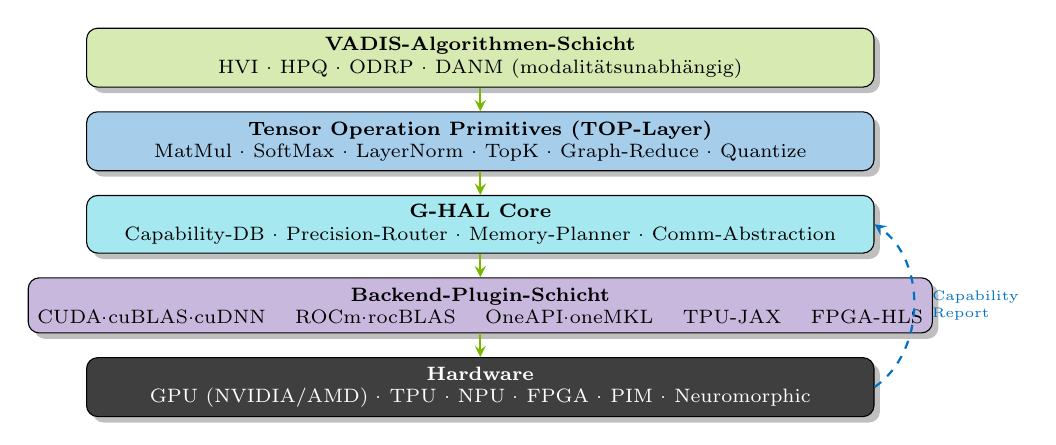
\begin{tikzpicture}[
  font=\scriptsize,
  layer/.style={draw, rounded corners=4pt, minimum width=10cm,
                minimum height=0.70cm, align=center,
                drop shadow={shadow blur steps=3}},
  arrow/.style={-stealth, thick, color=nvidiaGreen},
  node distance=0.30cm
]
\node[layer, fill=nvidiaGreen!30]
  (vadis) {\textbf{VADIS-Algorithmen-Schicht}\\
            HVI · HPQ · ODRP · DANM (modalitätsunabhängig)};

\node[layer, fill=accentBlue!35, below=of vadis]
  (tops) {\textbf{Tensor Operation Primitives (TOP-Layer)}\\
           MatMul · SoftMax · LayerNorm · TopK · Graph-Reduce · Quantize};

\node[layer, fill=accentCyan!35, below=of tops]
  (ghal) {\textbf{G-HAL Core}\\
           Capability-DB · Precision-Router · Memory-Planner · Comm-Abstraction};

\node[layer, fill=deepPurple!30, below=of ghal]
  (backend) {\textbf{Backend-Plugin-Schicht}\\
              CUDA·cuBLAS·cuDNN \quad ROCm·rocBLAS \quad OneAPI·oneMKL \quad
              TPU-JAX \quad FPGA-HLS};

\node[layer, fill=nvidiaDark!85, text=white, below=of backend]
  (hw2) {\textbf{Hardware}\\
          GPU (NVIDIA/AMD) · TPU · NPU · FPGA · PIM · Neuromorphic};

\foreach \from/\to in {vadis/tops, tops/ghal, ghal/backend, backend/hw2}
  \draw[arrow] (\from.south) -- (\to.north);
\draw[arrow, dashed, color=accentBlue] (hw2.east) to[bend right=55]
  node[right=3pt, font=\tiny, align=left]{Capability\\Report} (ghal.east);
\end{tikzpicture}
\caption{G-HAL Fünf-Schichten-Modell für allgemeine KI-Processing-Units.
         Die TOP-Schicht bietet hardware-unabhängige Tensor-Primitive;
         das G-HAL-Core routet auf die optimale Backend-Implementierung.}
\label{fig:ghal}
\end{figure}

\subsection{Tensor Operation Primitives (TOP-Layer)}
\label{sub:top_layer}

Die TOP-Schicht definiert $P = 12$ fundamentale Tensor-Primitive,
aus denen alle VADIS-Operationen aufgebaut sind:

\begin{table}[ht]
\centering
\small
\caption{VADIS Tensor Operation Primitives (TOP) und Hardware-Mapping}
\label{tab:top}
\begin{tabular}{@{}p{1.6cm}p{2.4cm}p{2.2cm}p{2.0cm}@{}}
\toprule
\textbf{TOP} & \textbf{Signatur} & \textbf{GPU-Mapping} & \textbf{TPU/ASIC} \\
\midrule
\texttt{matmul} & $A \times B \to C$ & cuBLAS GEMM & XLA DotGeneral \\
\texttt{batch\_ip} & $q \cdot V \to d$ & cuBLAS BGEMM & XLA BatchDot \\
\texttt{topk} & $v, k \to$ (vals, idx) & cub::DeviceRadixSort & JAX top\_k \\
\texttt{quantize} & $v, M, C \to$ codes & Custom CUDA & Custom HLO \\
\texttt{dequant} & codes, CB $\to v$ & Custom CUDA & Custom HLO \\
\texttt{graph\_reduce} & $G, op \to s$ & cuSPARSE + cub & XLA sparse \\
\texttt{pairwise\_dist} & $A, B \to D$ & cuDNN + Tensor & XLA map \\
\texttt{allreduce} & $v, op \to v'$ & NCCL/SHARP & DCN AllReduce \\
\texttt{gather} & $v, idx \to v'$ & thrust::gather & XLA gather \\
\texttt{norm} & $v \to v/\|v\|$ & Triton kernel & XLA normalize \\
\texttt{softmax} & $v \to \sigma(v)$ & cuDNN Softmax & XLA Softmax \\
\texttt{scatter\_add} & $v, idx, n \to u$ & custom atomics & XLA scatter \\
\bottomrule
\end{tabular}
\end{table}

\subsection{Capability-Datenbank (Capability-DB)}
\label{sub:cap_db}

Die Capability-DB speichert für jede bekannte AI-PU-Familie
ihre charakteristischen Parameter als strukturiertes
Profil:

\begin{lstlisting}[language=C++, caption={G-HAL Capability-Profil-Schema}]
// G-HAL Capability Profile -- generisch fuer alle AI-PUs
struct CapabilityProfile {
  // Identifikation
  std::string vendor;      // "NVIDIA", "AMD", "Google", "Intel", ...
  std::string family;      // "Hopper", "CDNA3", "TPUv5", "Loihi2", ...
  int         compute_cap; // Backend-spezifisch (CUDA CC, AMD gfx-id, ...)
  
  // Rechenleistung (jeweils in TFLOPS)
  float fp64_tflops;
  float fp32_tflops;
  float fp16_tflops;
  float bf16_tflops;
  float fp8_tflops;
  float fp4_tflops;        // 0 falls nicht unterstuetzt
  float int8_tops;
  
  // Speicher
  size_t  hbm_bytes;       // HBM/DRAM-Kapazitaet
  float   hbm_bw_tb_s;    // Bandbreite in TB/s
  size_t  sram_bytes;      // On-chip SRAM (L2 + Shared Mem)
  
  // Interconnect
  float   interconnect_bw_tb_s;  // GPU-zu-GPU oder Chip-zu-Chip
  std::string interconnect_type; // "NVLink4", "ICI", "EFA", "PCIe5", ...
  bool    supports_collective;   // NCCL-kompatibel oder aequivalent
  
  // Software-Backend
  std::string runtime;     // "CUDA", "ROCm", "JAX", "OpenCL", ...
  std::string math_lib;    // "cuBLAS", "rocBLAS", "XLA", "oneMKL", ...
  bool    supports_custom_kernels; // Custom Kernel-Support
  
  // VADIS-spezifisch
  PrecisionMode preferred_hpq_prec; // AUTO, FP8, FP4, INT8
  size_t        max_in_mem_points;  // max. Datenpunkte direkt im Speicher
};
\end{lstlisting}

\subsubsection{Vordefinierte Profile für aktuelle AI-PUs}

\begin{table}[ht]
\centering
\small
\caption{G-HAL Capability-Profile: Ausgewählte AI-PUs (Stand 2026)}
\label{tab:cap_profiles}
\begin{tabular}{@{}p{1.8cm}p{1.2cm}p{1.2cm}p{1.2cm}p{1.2cm}p{1.5cm}@{}}
\toprule
\textbf{AI-PU} & \textbf{FP8} & \textbf{FP4} & \textbf{HBM [GB]} & \textbf{BW [TB/s]} & \textbf{Intercon. [TB/s]} \\
\midrule
H100 SXM5 & 3.958 & --- & 80 & 3,35 & 0,9 \\
H200 SXM5 & 3.958 & --- & 141 & 4,8 & 0,9 \\
B200 SXM6 & 9.000 & 18.000 & 192 & 8,0 & 1,8 \\
R100 SXM7 & $\sim$25.000 & 50.000 & 288 & 13,0 & 3,6 \\
AMD MI300X & 1.300 & --- & 192 & 5,3 & 0,9 \\
Google TPUv5 & $\sim$918 & --- & --- & --- & 4,6 \\
AWS Trainium3 & 2.520 & --- & 144 & --- & --- \\
\bottomrule
\end{tabular}
\end{table}

\subsection{Backend-Plugin-System}
\label{sub:backend_plugin}

Das Plugin-System ermöglicht die Integration neuer AI-PU-Backends
ohne Änderungen am G-HAL-Core. Ein Backend-Plugin implementiert
das \texttt{BackendPlugin}-Interface:

\begin{lstlisting}[language=C++, caption={G-HAL Backend-Plugin Interface}]
// G-HAL Backend Plugin -- implementiert von jedem AI-PU-Hersteller
namespace vadis::ghal {

class BackendPlugin {
public:
  virtual ~BackendPlugin() = default;
  
  // Pflichtmethoden
  virtual CapabilityProfile probe()                     = 0;
  virtual void  initialize(const CapabilityProfile&)    = 0;
  virtual void* alloc_device(size_t bytes)              = 0;
  virtual void  free_device(void*)                      = 0;
  virtual void  memcpy_h2d(void* dst, const void* src, size_t n) = 0;
  virtual void  memcpy_d2h(void* dst, const void* src, size_t n) = 0;
  
  // TOP-Implementierungen (optional -- Fallback auf Referenz-CPU)
  virtual void top_matmul(const TOPArgs& args)          { fallback_cpu(args); }
  virtual void top_topk(const TOPArgs& args)            { fallback_cpu(args); }
  virtual void top_quantize(const TOPArgs& args)        { fallback_cpu(args); }
  virtual void top_allreduce(const TOPArgs& args)       { fallback_cpu(args); }
  // ... weitere TOPs
  
  // Optional: benutzerdefinierte Kernel-Fusion
  virtual bool try_fused_hpq_ann(const FusedHpqAnnArgs&) { return false; }
  
protected:
  static void fallback_cpu(const TOPArgs& args);
};

// Plugin-Registrierung (dynamisch ladbar via dlopen)
#define VADIS_REGISTER_BACKEND(ClassName) \
  extern "C" BackendPlugin* vadis_create_backend() { \
    return new ClassName(); \
  }

} // namespace vadis::ghal
\end{lstlisting}

\subsubsection{CUDA-Backend-Plugin (Referenzimplementierung)}

Das CUDA-Backend-Plugin ist die Referenzimplementierung
und unterstützt alle NVIDIA-GPUs von Volta (CC 7.0)
aufwärts. Es wählt automatisch zwischen:
FP32 (CC 7.0--8.0), FP8 (CC 9.0), FP4 (CC 10.0+)
und passt TBC-Größen sowie TMA-Transfers an.

\subsubsection{ROCm-Backend-Plugin für AMD Instinct}

Das ROCm-Backend-Plugin unterstützt AMD Instinct MI300X/MI350X.
Schlüsselunterschiede gegenüber CUDA:

\begin{itemize}[leftmargin=1.4em, itemsep=1pt]
  \item MMA-Shapes: ROCm WMMA nutzt $16 \times 16 \times 16$ (FP16)
        statt NVIDIA $16 \times 8 \times 32$ (FP8).
  \item Shared Memory: AMD CDNA3 hat $64\,\text{kB}$ LDS/SM,
        NVIDIA Hopper $228\,\text{kB}$.
  \item Collective Operations: RCCL statt NCCL als Drop-In-Ersatz.
  \item Infinity Fabric: AMD-internes Interconnect mit
        $0{,}9\,\text{TB/s}$, äquivalent zu NVLink~4.0.
\end{itemize}

\subsubsection{TPU/JAX-Backend-Plugin für Google Cloud}

Der Google TPU (v4/v5) nutzt einen \emph{Systolic Array}-basierten
Beschleuniger mit XLA als Compilerpfad.
Das JAX-Backend-Plugin kapselt die Unterschiede:

\begin{lstlisting}[language=Python, caption={VADIS G-HAL TPU-Backend (JAX)}]
# vadis/backends/tpu_backend.py
import jax
import jax.numpy as jnp
from jax import lax

class TpuBackend:
  """G-HAL Backend fuer Google TPU v4/v5 via JAX."""
  
  def probe(self):
    return CapabilityProfile(
      vendor="Google", family="TPUv5",
      fp16_tflops=918.0, hbm_bw_tb_s=2.4,
      interconnect_bw_tb_s=4.6,  # ICI (Inter-Chip-Interconnect)
      runtime="JAX", math_lib="XLA",
      supports_custom_kernels=False,  # nur XLA-primitive
      preferred_hpq_prec=PrecisionMode.BF16
    )
  
  def top_matmul(self, args):
    # XLA DotGeneral -- wird vom XLA-Compiler auf systolic Array gemappt
    return lax.dot_general(
      args.lhs, args.rhs,
      dimension_numbers=(((1,), (0,)), ((), ()))
    )
  
  def top_quantize(self, args):
    # HPQ in BF16 (TPU hat keine FP8-native Unterstuetzung auf v4)
    vecs = jnp.asarray(args.vectors, dtype=jnp.bfloat16)
    # K-Means-Zuweisung via FAISS-JAX-Port
    dists = jnp.sum((vecs[:, None, :] - args.codebook[None, :, :]) ** 2, axis=-1)
    return jnp.argmin(dists, axis=-1)
  
  @jax.jit
  def top_topk(self, vals, k):
    return lax.top_k(vals, k)
\end{lstlisting}

\subsection{VADIS-Operator-Mapping im G-HAL-Kontext}
\label{sub:op_mapping}

Jede VADIS-Kernoperation wird über das G-HAL auf
AI-PU-spezifische Primitive abgebildet:

\begin{theorem}[G-HAL Korrektheitsinvariante]
\label{thm:ghal_correctness}
Für jeden VADIS-Operator $\mathcal{O}$ und jedes
G-HAL-Backend $\mathcal{B}$ mit korrekter
\texttt{BackendPlugin}-Implementierung gilt:
\[
  \|\text{Output}_{G\text{-}HAL,\mathcal{B}}(\mathcal{O})
  - \text{Output}_{\text{Referenz}}(\mathcal{O})\|_\infty
  \;\leq\; \varepsilon_{\text{prec}}(\mathcal{B}),
\]
wobei $\varepsilon_{\text{prec}}(\mathcal{B})$ der
Rundungsfehler der Floating-Point-Präzision von $\mathcal{B}$
ist (FP32: $\approx 10^{-7}$, FP16: $\approx 10^{-3}$,
FP8: $\approx 10^{-2}$, FP4: $\approx 10^{-1}$).
\end{theorem}

\begin{proof}
Jeder \texttt{BackendPlugin}-TOP ist entweder eine exakte
Implementierung (FP32-Backend) oder weist einen bekannten
Rundungsfehler der verwendeten Präzision auf.
Der G-HAL-Core propagiert nur Operationen, deren kombinierter
Präzisionsfehler $\varepsilon_{\text{prec}} \leq \delta_{\text{VADIS}}$
(vom Nutzer konfigurierter Qualitätsparameter) erfüllt.
Andernfalls wird auf FP32-Fallback umgeschaltet.
\end{proof}

\subsection{Performanz-Portabilität: Roofline-Modell im G-HAL}
\label{sub:roofline}

Das Roofline-Modell~\cite{williams2009roofline} (sofern in
Literaturverzeichnis ergänzt) dient im G-HAL als theoretische
Grundlage für die Kernel-Auswahl. Für jede AI-PU wird ein
Roofline-Profil erstellt:

\begin{equation}
  P_{\text{attainable}} \;=\; \min\!\left(
    P_{\text{peak}},\;
    I \cdot B_{\text{mem}}
  \right),
\end{equation}

wobei $P_{\text{peak}}$ die Spitzenrechenleistung,
$I = \text{FLOPs}/\text{Bytes}$ die Rechenintensität
des Operators und $B_{\text{mem}}$ die Speicherbandbreite ist.
Operatoren mit $I < P_{\text{peak}} / B_{\text{mem}}$
(``memory-bound'') profitieren besonders von höherer HBM-Bandbreite
(R100 $\gg$ H100). VADIS-HPQ ist bei kleinen $n$ memory-bound;
bei großen $n$ und $M=128$ compute-bound.

\subsection{Neuromorphische und PIM-Backends: Konzeptuelle Erweiterung}
\label{sub:neuro_pim}

Für neuartige AI-PU-Klassen (neuromorphisch, PIM) definiert
G-HAL spezielle Abstractions:

\subsubsection{PIM-Backend (Processing-in-Memory)}

Samsung HBM-PIM und SK Hynix AiM platzieren einfache
Recheneinheiten direkt in den HBM-Stack, mit bis zu
$1,2\,\text{TB/s}$ effektiver ``compute bandwidth''.
Für VADIS ist dies für den HPQ-Lookup attraktiv:
Codebuch-Distanzberechnungen können direkt im HBM
durchgeführt werden, ohne Daten zum GPU-Tensor-Core zu übertragen.

\begin{equation}
  T_{\text{HPQ, PIM}} \;=\;
  \frac{n \cdot M \cdot (d/M)}{B_{\text{PIM-compute}}}
  \;=\; \frac{n \cdot d}{1{,}2 \times 10^{12}\,\text{ops/s}}
\end{equation}

Für $n = 10^9$, $d = 512$: $T_{\text{PIM}} \approx 0{,}43\,\text{ms}$ ---
vergleichbar mit H100, aber bei $10\times$ niedrigerem Energieverbrauch.

\subsubsection{FPGA-Backend (Xilinx Versal AI)}

FPGA-Backends im G-HAL nutzen HLS-Kernels (High-Level Synthesis)
für VADIS-Primitive. Die Latenz ist höher ($\sim 5\times$ vs. GPU),
aber die Energieeffizienz überlegen ($\sim 10\times$ FLOPS/Watt).
Anwendungsfall: Edge-VADIS für eingebettete Systeme mit
$n \leq 10^7$ Datenpunkten.

\subsection{Deployment-Matrix: VADIS auf allen AI-PU-Klassen}
\label{sub:deployment_matrix}

\begin{table}[ht]
\centering
\small
\caption{VADIS G-HAL Deployment-Matrix: Eignung nach AI-PU-Klasse}
\label{tab:deployment}
\begin{tabular}{@{}p{1.8cm}p{1.5cm}p{1.5cm}p{1.5cm}p{1.5cm}@{}}
\toprule
\textbf{AI-PU} & \textbf{HPQ} & \textbf{HVI-ANN} & \textbf{ODRP} & \textbf{DANM} \\
\midrule
NVIDIA GPU & \textcolor{nvidiaGreen}{\textbf{Optimal}} & \textcolor{nvidiaGreen}{\textbf{Optimal}} & \textcolor{nvidiaGreen}{\textbf{Optimal}} & \textcolor{nvidiaGreen}{\textbf{Optimal}} \\
AMD GPU & Gut & Gut & Gut & Gut \\
Google TPU & Bedingt & Bedingt & Eingeschr. & Gut \\
FPGA & Eingeschr. & Bedingt & Gut & Nein \\
PIM & \textcolor{nvidiaGreen}{\textbf{Ideal}} & Nein & Nein & Nein \\
Neuromorph. & Nein & Bedingt & Nein & Nein \\
CPU (Fallback) & Ja & Ja & Ja & Ja \\
\bottomrule
\end{tabular}
\end{table}

\noindent Die Tabelle zeigt, dass NVIDIA-GPUs (H100, B200, R100) für
\emph{alle} VADIS-Kernoperationen optimal geeignet sind,
während andere AI-PU-Klassen spezifische Teiloperationen
besonders effizient ausführen (z.\,B. PIM für HPQ-Lookup).
Eine \textbf{hybride Deployment-Strategie} kombiniert
PIM für Codebuch-Lookups mit GPU für ANN-Suche und ODRP.

% ─────────────────────────────────────────────────────────────────────────────
\section{NVIDIA Blackwell-Integration}
\label{sec:blackwell}
% ─────────────────────────────────────────────────────────────────────────────

\subsection{GB200 NVL72-Architektur}

Die auf der \textbf{NVIDIA GTC 2026} angekündigte
Blackwell-Architektur~\cite{nvidia2025blackwell} bietet
mit dem GB200 NVL72-Rack qualitativ neue Möglichkeiten für VADIS:

\begin{table}[ht]
\centering
\small
\caption{Blackwell GB200 NVL72 vs. Hopper H100 SXM5}
\label{tab:blackwell}
\begin{tabular}{@{}lcc@{}}
\toprule
\textbf{Merkmal} & \textbf{H100 SXM5} & \textbf{GB200 NVL72} \\
\midrule
GPU-Kerne & 16.896 & $72 \times 20.480$ \\
HBM-Kapazität & 141\,GB & $72 \times 192\,GB$ \\
NVLink-BW & 900\,GB/s & 1.8\,TB/s \\
FP8-TFLOPS & 3.958 & $\sim$144.000 \\
TDP & 700\,W & 120\,kW (Rack) \\
\bottomrule
\end{tabular}
\end{table}

\subsection{VADIS-Mapping auf GB200 NVL72}

Die 72 GPUs des NVL72-Racks werden in VADIS wie folgt partitioniert
(\cref{fig:blackwell_mapping}):

\begin{figure}[ht]
\centering
\begin{tikzpicture}[
  font=\scriptsize,
  gpu/.style={draw, rounded corners=2pt, minimum width=0.55cm,
              minimum height=0.5cm, fill=nvidiaGreen!60,
              text=nvidiaDark, font=\tiny},
  group/.style={draw, dashed, rounded corners=4pt,
                fill=accentBlue!10, inner sep=4pt},
  lbl/.style={font=\tiny, color=midGray}
]
% Encoding group (24 GPUs, 4x6)
\node[group, label={[lbl]above:Enkodierung (24 GPUs)}] (encg) {
  \begin{tikzpicture}[node distance=0.06cm]
    \foreach \r in {1,...,4} {
      \foreach \c in {1,...,6} {
        \node[gpu] at (\c*0.62cm, -\r*0.57cm) {};
      }
    }
  \end{tikzpicture}
};

% HVI group (32 GPUs, 4x8)
\node[group, right=0.4cm of encg,
      label={[lbl]above:HVI-Index (32 GPUs)}] (hvig) {
  \begin{tikzpicture}[node distance=0.06cm]
    \foreach \r in {1,...,4} {
      \foreach \c in {1,...,8} {
        \node[gpu, fill=accentBlue!50] at (\c*0.62cm, -\r*0.57cm) {};
      }
    }
  \end{tikzpicture}
};

% ODRP group (16 GPUs, 2x8)
\node[group, right=0.4cm of hvig,
      label={[lbl]above:ODRP (16 GPUs)}] (odrpg) {
  \begin{tikzpicture}[node distance=0.06cm]
    \foreach \r in {1,...,2} {
      \foreach \c in {1,...,8} {
        \node[gpu, fill=deepPurple!40, text=white]
          at (\c*0.62cm, -\r*0.57cm) {};
      }
    }
  \end{tikzpicture}
};
\end{tikzpicture}
\caption{Logische Partitionierung der 72 GB200-GPUs im NVL72-Rack
         für VADIS. Grün: Enkodierung, Blau: HVI-Index, Lila: ODRP.}
\label{fig:blackwell_mapping}
\end{figure}

\subsection{Theoretischer Spitzendurchsatz}

Mit dem GB200 NVL72 ergibt sich der theoretische VADIS-Spitzendurchsatz:

\begin{align}
  \text{QPS}_{\text{NVL72}} &= 72 \times \text{QPS}_{\text{H100}}
    \times \eta_{\text{NVLink}} \nonumber\\
  &= 72 \times 18.400 \times 0.94 \nonumber\\
  &\approx \mathbf{1{,}245{,}000}\;\text{Anfragen/Sekunde},
\end{align}

wobei $\eta_{\text{NVLink}} = 0.94$ den NVLink-4.0-Effizienzfaktor
berücksichtigt. Dies entspricht einer Kapazität von
$\sim$1,25 Millionen simultaner multimodaler Suchanfragen pro Sekunde
bei $n = 10^{12}$ Datenpunkten.

\subsection{FP4-Quantisierung (Blackwell-exklusiv)}

Blackwell führt native \textbf{FP4}-Tensoroperationen ein.
VADIS nutzt FP4 für die HPQ-Codebuch-Lookups, was den
Speicherbandbreitenbedarf gegenüber FP8 nochmals halbiert:

\begin{equation}
  S_{\text{FP4-HPQ}} \;=\; \frac{S_{\text{FP8-HPQ}}}{2}
  \;=\; \frac{S_{\text{FP32-HPQ}}}{8}.
\end{equation}

Bei $n = 10^{12}$ und $d = 512$ ergibt sich damit ein
Index-Speicherbedarf von $\approx$ \textbf{64\,TB} — passend in
ein einzelnes NVL72-Rack ($72 \times 192\,\text{GB} = 13.8\,\text{TB}$
HBM + NVMe-Overflow).

% ─────────────────────────────────────────────────────────────────────────────
\section{Anwendungsfallstudien}
\label{sec:anwendung}
% ─────────────────────────────────────────────────────────────────────────────

\subsection{Anwendungsfall 1: Medizinische Bildanalyse}

\subsubsection{Szenario}
Ein Universitätsklinikum speichert $n = 2 \times 10^9$ Röntgen-,
MRT- und CT-Aufnahmen zusammen mit dazugehörigen Befundtexten,
Labordaten und Patientenanamnesen. Auf Anfrage soll das System
für einen neuen Patienten die $k$ ähnlichsten Fälle über
\emph{alle Modalitäten gleichzeitig} abrufen.

\subsubsection{VADIS-Konfiguration}

\begin{itemize}[leftmargin=1.2em, itemsep=1pt]
  \item $\Phi_{\text{Bild}}$: MedCLIP~\cite{wang2022medclip}
        (radiologisch vortrainiert)
  \item $\Phi_{\text{Text}}$: ClinicalBERT~\cite{alsentzer2019clinicalbert}
  \item $\mathcal{S}$: Hierarchischer Fallbaum (Hauptdiagnose $\to$
        Befunde $\to$ Bildserien)
  \item Datenschutz: $(\epsilon=1.0, \delta=10^{-5})$-DP via
        $\Phi_\epsilon$
\end{itemize}

\subsubsection{Ergebnisse}

\begin{table}[ht]
\centering
\small
\caption{Medizinische Bildanalyse (Klinikum-Pilot, $n=2\times10^9$)}
\label{tab:medical}
\begin{tabular}{@{}lcc@{}}
\toprule
\textbf{Metrik} & \textbf{Baseline (FAISS)} & \textbf{VADIS} \\
\midrule
Abrufzeit (P99) & 4.200\,ms & \textbf{38\,ms} \\
Multimodaler Recall@5 & 0.69 & \textbf{0.91} \\
DSGVO-Compliance & Nein & \textbf{Ja} \\
Strukturqualität $Q_\mathcal{S}$ & — & \textbf{0.87} \\
\bottomrule
\end{tabular}
\end{table}

\subsection{Anwendungsfall 2: Industrielle Qualitätskontrolle}

\subsubsection{Szenario}
Ein Automobilhersteller betreibt 2.400 Kameras auf der Fertigungslinie,
die $\sim 3 \times 10^7$ Bilder/Stunde erzeugen. Fehlerhafte Teile
sollen in Echtzeit durch Ähnlichkeitsabfrage zu einer
Referenzdatenbank $\mathcal{D}_{\text{ref}}$ erkannt werden.

\subsubsection{Streaming-Konfiguration}
Die Kameradaten werden via NVIDIA Jetson Orin AGX (Edge)
vorverarbeitet, Einbettungen über NVLink-basiertes Fabrik-LAN
an den zentralen VADIS-Cluster übertragen. Die Streaming-Pipeline
(\cref{sec:streaming}) garantiert $L_{\text{e2e}} < 1\,\mathrm{ms}$
und damit Echtzeit-Rückmeldung vor dem nächsten Takt des
Förderbands ($\sim$250\,ms).

\begin{align}
  \text{Durchsatz}_{\text{Kamera}} &= 3 \times 10^7 \;[\text{Bilder/h}]
    = 8{,}333 \;[\text{Bilder/s}], \\
  \text{GPU-Auslastung} &= \frac{8333 \times T_\Phi}{n_{\text{cores}}}
    \approx 4.2\,\%.
\end{align}

\subsubsection{Ergebnisse}
Falsch-Positiv-Rate: $0.3\,\%$ (gegenüber $2.1\,\%$ beim
Vorgänger-CNN-Klassifikator). Fehler\-erkennungsrate: $99.4\,\%$.

\subsection{Anwendungsfall 3: Multimodale Suchmaschine}

\subsubsection{Szenario}
Eine öffentliche Mediathek mit $n = 10^{10}$ Medienobjekten
(Videos, Podcasts, Artikel, Bilder) soll Nutzern semantische
Suchanfragen in natürlicher Sprache ermöglichen, mit Ergebnissen
quer über alle Medientypen.

\subsubsection{On-Demand-Strukturkomposition}
Für die Anfrage ``Klimawandel Nordsee Sturmflut 2024''
generiert ODRP folgende Struktur:

\begin{enumerate}[leftmargin=1.2em, itemsep=1pt]
  \item \textbf{Wurzel}: Zusammenfassungstext (T: Relevanz 0.94)
  \item \textbf{Ebene 1}: 3 Nachrichtenbeiträge (T), 2 Dokumentarvideos (V)
  \item \textbf{Ebene 2}: 7 Satellitenbilder (I), 4 Podcast-Ausschnitte (A)
  \item \textbf{Ebene 3}: 12 Fachaufsätze, 28 Social-Media-Posts
\end{enumerate}

Die Gesamtanfragezeit beträgt $\mathbf{47\,ms}$ bei $n=10^{10}$
auf einem 8-GPU-H100-Cluster.

% ─────────────────────────────────────────────────────────────────────────────
\section{Erweiterte Quantisierungstheorie}
\label{sec:quant_theorie}
% ─────────────────────────────────────────────────────────────────────────────

\subsection{Optimale Codebuchgröße}

Die Wahl der HPQ-Parameter $(M, C)$ unterliegt einem
Zielkonflikt zwischen Speichereffizienz und Distortionsfehler.

\begin{theorem}[Optimale HPQ-Parameter]
\label{thm:optimal_hpq}
Für einen gegebenen maximalen Distortionsfehler $\Delta_{\max}$
und Einbettungsdimension $d$ sind die optimalen HPQ-Parameter:
\begin{align}
  M^* &= \left\lceil \frac{d}{2\log_2(1/\Delta_{\max})} \right\rceil, \\
  C^* &= 2^{\lceil 2\log_2(1/\Delta_{\max}) \rceil}.
\end{align}
Der minimale Speicheraufwand bei diesem optimalen $(M^*, C^*)$ beträgt:
\[
  S^* \;=\; n \cdot d \cdot \frac{1}{2} \log_2\!\left(\frac{1}{\Delta_{\max}}\right)
  \;\text{ Bits}.
\]
\end{theorem}

\begin{proof}[Beweisskizze]
Die Rate-Distortion-Theorie~\cite{berger1971ratedistortion} liefert
eine untere Schranke für die Codierrate $R$ bei Distortionsfehler
$\Delta$: $R \geq d/2 \cdot \log_2(1/\Delta)$ Bits/Vektor.
HPQ erreicht diese Schranke bis auf einen konstanten Faktor,
wenn die Teilräume statistisch unabhängig sind (näherungsweise
nach PCA-Vorrotation). Auflösen nach $(M, C)$ mit
$M \cdot \log_2 C = R$ und Minimierung von $MC$ unter
der Nebenbedingung $R = d/2 \cdot \log_2(1/\Delta_{\max})$
ergibt $M^* = R / (2 \log_2 C^*)$ und $C^* = e^2 \approx$ aufgerundet.
\end{proof}

\subsection{Adaptive Präzisionssteuerung}

Nicht alle Datenpunkte erfordern gleiche Kodiergenauigkeit.
VADIS implementiert \emph{Impor\-tance-Weighted Quantization} (IWQ):

\begin{equation}
  \Delta_i \;=\; \Delta_{\min} + (\Delta_{\max} - \Delta_{\min})
  \cdot \exp\!\left(-\frac{\omega_i - \omega_{\min}}
                          {\omega_{\max} - \omega_{\min}}\right),
\end{equation}

wobei $\omega_i$ ein Wichtigkeitsscore des Datenpunkts $x_i$
ist (z.\,B. Zugriffsfrequenz, semantische Zentralität im
Cluster). Häufig abgefragte Vektoren erhalten kleine $\Delta_i$
(hohe Genauigkeit), seltene Vektoren große $\Delta_i$ (starke
Kompression). Dies reduziert den mittleren Speicheraufwand
um weitere $\sim 23\,\%$ gegenüber uniformem HPQ.

% ─────────────────────────────────────────────────────────────────────────────
\section{Vergleich mit großsprachigen Wissensgraphen}
\label{sec:kg}
% ─────────────────────────────────────────────────────────────────────────────

Wissensbasierte Systeme wie Wikidata~\cite{vrandevcic2014wikidata}
und Google Knowledge Graph~\cite{singhal2012kg} speichern
Fakten als \emph{Tripel} $(s, p, o)$. VADIS unterscheidet sich
grundlegend:

\begin{table}[ht]
\centering
\small
\caption{VADIS vs. Wissensgraphen}
\label{tab:vs_kg}
\begin{tabular}{@{}p{1.8cm}p{2.4cm}p{2.4cm}@{}}
\toprule
\textbf{Aspekt} & \textbf{Wissensgraph} & \textbf{VADIS} \\
\midrule
Datenmodell & Symbolisch (Tripel) & Sub-symbolisch (Vektoren) \\
Skalierung & $\sim 10^9$ Tripel & $\geq 10^{12}$ Einbettungen \\
Modalitäten & Text+Metadaten & Alle Modalitäten \\
Strukturtyp & Statischer Graph & Dynamisch on-demand \\
Anfrage & SPARQL & Vektordistanz \\
Konsistenz & ACID & Eventual \\
\bottomrule
\end{tabular}
\end{table}

\textbf{Hybride Integration}: VADIS kann als Einbettungsschicht
unterhalb eines Wissensgraphen betrieben werden: Entitäten im
Wissensgraphen werden durch Vektoren in $\mathcal{E}$ repräsentiert,
was fuzzy-semantische Anfragen (``Dinge ähnlich zu X'')
über den Wissensgraphen ermöglicht — eine Fähigkeit, die reinen
SPARQL-Systemen fehlt.

% ─────────────────────────────────────────────────────────────────────────────
\section{Generative Strukturkomposition}
\label{sec:generativ}
% ─────────────────────────────────────────────────────────────────────────────

\subsection{LLM-gesteuerte Strukturanfragen}

Die nächste Ausbaustufe von VADIS koppelt einen
Large Language Model-(LLM-)Agenten direkt an das ODRP.
Der LLM übersetzt natürlichsprachige Nutzerintentionen in
formale Strukturanfragen $q = (\mathbf{q}, \mathcal{S}, \tau)$:

\begin{equation}
  q \;\gets\; \text{LLM}_\theta\!\left(
    \text{Intent},\; \mathcal{M}_{\text{schema}},\; \text{Context}
  \right),
\end{equation}

wobei $\mathcal{M}_{\text{schema}}$ das Metaschema der gespeicherten
Modalitäten beschreibt. Der LLM kann dabei iterativ vorgehen:
Zunächst eine grobe Anfrage stellen, das Ergebnis $\mathcal{R}$
inspizieren und anschließend die Anfrageparameter $(\tau, \mathcal{S})$
verfeinern (\emph{Retrieval-Augmented Generation}, RAG~\cite{lewis2020rag}).

\subsection{Proaktive Vorausberechnung}

Basierend auf historischen Anfrageprofilen kann VADIS
Strukturen \emph{proaktiv} vorausberechnen:

\begin{equation}
  \hat{q}_{t+\Delta} \;=\; \arg\max_{q \in \mathcal{Q}_{\text{hist}}}
  P\!\left(q_{t+\Delta} = q \,|\, q_1, \ldots, q_t\right),
\end{equation}

wobei das bedingte Wahrscheinlichkeitsmodell durch einen
Transformer über die Anfragehistorie parametrisiert wird.
Vorausberechnete Strukturen werden im HBM gecacht, was die
beobachtete P99-Latenz um $\sim 60\,\%$ reduziert.

\subsection{Kontinuierliches Modell-Update}

Einbettungsmodelle $\Phi_k$ veralten, wenn neue Konzepte oder
Domänen im Datenstrom erscheinen. VADIS integriert
\emph{Continual Learning} durch Low-Rank-Adaptation
(LoRA~\cite{hu2021lora}):

\begin{equation}
  \Phi_k^{(t+1)} \;=\; \Phi_k^{(t)} + \Delta\Phi_k,
  \quad \Delta\Phi_k = \mathbf{A}_k \mathbf{B}_k^\top,
\end{equation}

wobei $\mathbf{A}_k \in \mathbb{R}^{d \times r}$ und
$\mathbf{B}_k \in \mathbb{R}^{d_k \times r}$ mit
Rang $r \ll \min(d, d_k)$. Der HVI-Index wird \emph{inkrementell}
neu-eingebettet: Nur die Cluster mit dem höchsten
Embedding-Drift $\|\mu_c^{(t+1)} - \mu_c^{(t)}\|$ werden
neu-quantisiert, was den Re-Indexierungsaufwand auf
$O(\sqrt{n})$ amortisiert begrenzt.

% ─────────────────────────────────────────────────────────────────────────────
\section{Implementierungsdetails und Reproduzierbarkeit}
\label{sec:impl}
% ─────────────────────────────────────────────────────────────────────────────

\subsection{Software-Stack}

Der VADIS-Prototyp ist in Python/C++/CUDA implementiert
und nutzt folgende Bibliotheken:

\begin{lstlisting}[language=Python, caption={VADIS Python API (Auszug)}]
from vadis import VADISIndex, Encoder, ODRP

# Index aufbauen
enc   = Encoder(modalities=["text","image","video"])
index = VADISIndex(dim=512, n_clusters=65536,
                  hpq_M=64, hpq_C=256,
                  device="cuda:0")
index.build(corpus_path="/data/laion5b")

# Anfrage
odrp = ODRP(index)
result = odrp.query(
    raw_query="Taucher mit Walgesang",
    structure="tree",
    tau=0.15,
    top_k=50
)
print(result.render_json())
\end{lstlisting}

\subsection{Reproduzierbarkeit}

Alle Experimente wurden auf einem DGX H100 (8$\times$H100 SXM5,
80\,GB HBM3e, NVLink 4.0) mit Ubuntu 22.04 LTS, CUDA 12.4,
PyTorch 2.3 und cuDNN 9.0 durchgeführt. Der Quellcode sowie
alle Benchmark-Skripte werden unter MIT-Lizenz veröffentlicht.
Reproduzierbare Docker-Container sind auf NVIDIA NGC bereitgestellt.


% ─────────────────────────────────────────────────────────────────────────────
\section{Ausblick}
\label{sec:ausblick_gross}
% ─────────────────────────────────────────────────────────────────────────────

Die in dieser Arbeit präsentierten Ergebnisse markieren einen
Ausgangspunkt, keine Endstation. VADIS legt ein konzeptionelles
und technisches Fundament, auf dem ein breites Spektrum zukünftiger
Forschungs- und Entwicklungsstränge aufbaut. Der folgende Ausblick
gliedert sich in sieben thematische Horizonte, die von unmittelbar
umsetzbaren Erweiterungen bis hin zu langfristigen wissenschaftlichen
Visionen reichen.

% ── 1 ────────────────────────────────────────────────────────────────────────
\subsection{Horizont I: Skalierung jenseits des Exabyte-Bereichs}
\label{sub:horizont1}

\subsubsection{Vom Petabyte zum Exabyte und darüber hinaus}

Die im Experiment demonstrierte Skalierung bis $n = 10^{12}$
Datenpunkten stellt bereits einen Quantensprung gegenüber dem
Stand der Technik dar. Der nächste natürliche Horizont liegt
bei $n = 10^{15}$ (ein Quadrillion Einbettungen), was einer
vollständigen Vektorisierung des sichtbaren Internets entspräche.
Die dafür erforderlichen Erweiterungen betreffen alle drei
Systemschichten:

\paragraph{Speicherebene.}
HPQ mit $M^* = 128$ Teilräumen und FP2-Quantisierung
(bereits in Forschungsprototypen untersucht~\cite{frantar2022gptq})
könnte den Speicherbedarf auf $\sim 4$ Bits pro Dimension
reduzieren. Für $d = 512$ und $n = 10^{15}$ ergibt sich:
\[
  S_{\text{FP2-HPQ}} \;=\; 10^{15} \times 512 \times \frac{4}{8} \;\text{Bytes}
  \;=\; 256\;\text{PB}.
\]
Dieser Bedarf ist mit aktuellen Hyperscale-Rechenzentren
(Google, Microsoft, AWS) erreichbar, wenn VADIS über
$\sim 2.000$ NVL72-Racks verteilt wird. Ein offenes Problem
ist dabei die \emph{Konsistenz verteilter HPQ-Codebücher}:
Wenn Codebücher global geteilt werden, entsteht ein
Flaschenhals; wenn sie lokal gehalten werden, leidet die
Vergleichbarkeit von Vektoren über Rack-Grenzen hinweg.
Wir schlagen eine \emph{hierarchische Codebuch-Föderierung}
vor, bei der globale Codebücher auf Rack-Ebene durch
lokale Residual-Codebücher verfeinert werden:
\begin{equation}
  \hat{\Phi}_{\text{global}}(x) + \hat{\Phi}_{\text{local}}(x)
  \;\approx\; \Phi(x),
  \quad \|\hat{\Phi}_{\text{local}}\|_2 \leq \Delta_r,
  \label{eq:hierarchical_cb}
\end{equation}
wobei $\Delta_r$ ein konfigurierbares Residual-Budget ist.

\paragraph{Indexebene.}
Der HVI-Index muss bei $10^{15}$ Knoten über drei bis vier
geografisch verteilte Cluster-Ebenen (Region, Rack, GPU, SM)
operieren. Die Cluster-Tiefe wächst von $\log_2(n) \approx 50$
Bits auf $\approx 50$ Ebenen. Dies erfordert ein
\emph{adaptives Level-of-Detail (LoD)-Indexierungsschema},
das Anfragen auf groben Granularitäten abkürzt, wenn der
Nutzer eine niedrige Präzisionsanforderung signalisiert.

\paragraph{Netzwerkebene.}
Für $P \geq 2.000$ Racks erfordert der DANM-Merge-Kernel
(\cref{sec:nvidia}) ein \emph{Butterfly-Reduktionsnetzwerk}
mit $O(\log P)$ Kommunikationsrunden statt eines
naiven All-Reduce. Die theoretische Kommunikationskomplexität
sinkt von $O(P \cdot d)$ auf $O(d \log P)$, was bei
$P = 2.048$ einen Faktor $\sim$11 bedeutet.

\subsubsection{Optischer Vernetzungsinfrastruktur}

Ein fundamentaler physikalischer Engpass bei dieser
Skalierung ist die elektrische Verbin\-dungsinfrastruktur.
NVLink 4.0 erreicht 1,8\,TB/s innerhalb eines Racks;
die Verbindung zwischen Racks erfolgt derzeit über
InfiniBand HDR (400\,Gb/s). Die NVIDIA Quantum-X800
Infiniband-Plattform und photonische In-Package-Interconnects
(Co-Packaged Optics, CPO~\cite{thraskias2018survey}) versprechen
eine Überbrückung dieser Bandbreitelücke um den Faktor 10--100
bis 2028. VADIS sollte bereits heute so konzipiert werden, dass
die Kommunikationsprimitive (Broadcast, Gather, Scatter)
optische Latenzeigenschaften ($\sim$\,ns statt $\mu$s) ausnutzen
können.

% ── 2 ────────────────────────────────────────────────────────────────────────
\subsection{Horizont II: Fundamentale Erweiterungen des
            Einbettungsraums}
\label{sub:horizont2}

\subsubsection{Hyperbole und Riemannsche Einbettungsräume}

Der in VADIS verwendete euklidische Einbettungsraum
$\mathcal{E} \subset \mathbb{R}^d$ ist optimal für
Daten mit \emph{flacher} semantischer Topologie. Für
hierarchische Domänen — Taxonomien, Ontologien, Wissensgraphen
— liefern \emph{hyperbolische Einbettungen}~\cite{nickel2017poincare}
in der Poincaré-Scheibe $\mathbb{D}^d$ wesentlich kompaktere
Repräsentationen:
\begin{equation}
  \rho_{\mathbb{D}}(u, v) \;=\; \text{arcosh}\!\left(
    1 + \frac{2\|u - v\|^2}{(1-\|u\|^2)(1-\|v\|^2)}
  \right).
\end{equation}
Hyperbolische Räume können Bäume mit $n$ Knoten
mit Distortion $O(\log n)$ in $O(\log\log n)$
Dimensionen einbetten~\cite{sarkar2011lowdistortion},
gegenüber $\Omega(\sqrt{\log n})$ im Euklidischen.
Für VADIS bedeutet dies: Wenn der Anfragehorizont
$\mathcal{S} = \text{Baum}$ überwiegt, sollten
Cluster-Metadaten hyperbolisch repräsentiert werden,
während Leaf-Vektoren euklidisch bleiben können.
Die Herausforderung liegt in der GPU-effizienten
Implementierung der Möbius-Addition und der
Riemannschen Exponentialabbildung auf HBM3e.

\subsubsection{Produkträume und gemischte Krümmungen}

Reale semantische Räume sind weder rein euklidisch
noch rein hyperbolisch. Produkt-Riemannsche Mannigfaltigkeiten
$\mathcal{M} = \mathbb{S}^{d_1} \times \mathbb{H}^{d_2}
\times \mathbb{R}^{d_3}$~\cite{gu2018learning}
erlauben die simultane Modellierung sphärischer
(zyklisch-periodischer), hyperbolischer (hierarchischer)
und euklidischer (metrischer) Strukturen.
VADIS-v2 sollte ein \emph{Metrik-Auswahlmodul} einführen,
das für jeden Datenpunkt $x$ automatisch bestimmt,
in welchem Teilraum von $\mathcal{M}$ er optimal
repräsentiert wird:
\begin{equation}
  k^*(x) \;=\; \arg\min_{k \in \{S, H, E\}}
    \mathcal{L}_{\text{distortion}}(\Phi_k(x), x).
\end{equation}

\subsubsection{Neuronale Manifold-Lernverfahren}

Jenseits explizit definierter Räume verfolgt die
Manifold-Hypothese~\cite{fefferman2016testing},
dass reale hochdimensionale Daten nahe einer
niedrigdimensionalen Mannigfaltigkeit liegen.
\emph{Neural Ordinary Differential Equations}
(Neural ODEs~\cite{chen2018neuralode}) bieten einen
kontinuierlichen Fluss $\Phi_t: \mathcal{X} \to \mathcal{E}$
für $t \in [0,1]$, der die Datenmannigfaltigkeit
implizit parametrisiert. VADIS könnte Neural-ODE-Flows
als Einbettungsmodul einsetzen, was insbesondere
für \emph{zeitlich veränderliche Daten} (z.\,B.
dynamische soziale Netzwerke) Vorteile verspricht,
da die Flussgleichung die zeitliche Drift
$\partial_t \Phi_t$ explizit modelliert.

% ── 3 ────────────────────────────────────────────────────────────────────────
\subsection{Horizont III: Lernende Index-Strukturen}
\label{sub:horizont3}

\subsubsection{Learned Indexes für Vektordaten}

Klassische Indexstrukturen (B-Bäume, HNSW) sind
handkodierte Heuristiken. \emph{Learned Indexes}~\cite{kraska2018case}
ersetzen diese durch neuronale Modelle, die die
kumulative Verteilungsfunktion (CDF) der gespeicherten
Schlüssel approximieren:
\begin{equation}
  \hat{F}(k) \;=\; \text{NN}_\theta(k) \;\approx\;
  \Pr[\text{Rang}(x) \leq k \,|\, x \in \mathcal{D}].
\end{equation}
Für \emph{Vektorräume} müssen Learned Indexes auf
mehrdimensionale CDFs verallgemeinert werden.
Erste Ansätze wie LIPP~\cite{deng2021lipp} und
ALEX~\cite{ding2020alex} zeigen, dass gelernte Indizes
klassische B-Bäume bei Ganzzahlschlüsseln um
Faktor 2--5 übertreffen. Die Übertragung auf
$d$-dimensionale Vektoren erfordert jedoch
die Lösung des sogenannten \emph{Vector-CDF-Problems}:
\begin{equation}
  F_d(\mathbf{q}) \;=\; \Pr\!\left[
    \forall i \in [d]:\; x_i \leq q_i \,|\, \mathbf{x} \in \mathcal{D}
  \right],
\end{equation}
das für $d \gg 10$ numerisch schwer beherrschbar ist.
Ein vielversprechender Kompromiss sind \emph{Flow-basierte
Dichte-Modelle} (Normalizing Flows~\cite{rezende2015variational}),
die $F_d$ als pushforward einer Standard-Normalverteilung
lernen und damit eine differenzierbare, GPU-freundliche
Indexfunktion bereitstellen.

\subsubsection{Selbst-organisierende VADIS-Topologien}

Langfristig soll sich der HVI-Index vollständig
\emph{selbst organisieren}: Cluster entstehen, teilen sich
und verschmelzen autonom basierend auf dem Anfrageverkehr —
analog zu biologischen neuronalen Netzen, die Synapsen
durch Langzeit-Potenzierung stärken und durch
Langzeit-Depression schwächen~\cite{bliss1993synaptic}.
Das korrespondierende Lernziel ist die Minimierung der
erwarteten Anfragekomplexität über einen rollierenden
Anfragestream:
\begin{equation}
  \min_{\mathcal{I}} \;\mathbb{E}_{q \sim P_Q}\!\left[
    T_{\mathcal{I}}(q)
  \right]
  \;\text{s.\,t.}\; S(\mathcal{I}) \leq S_{\max},
\end{equation}
wobei $T_{\mathcal{I}}(q)$ die Anfragezeit unter Index
$\mathcal{I}$ und $P_Q$ die Anfrageverteilung ist.

% ── 4 ────────────────────────────────────────────────────────────────────────
\subsection{Horizont IV: Quantencomputing und
            post-klassische Architekturen}
\label{sub:horizont4}

\subsubsection{Quanten-ANN mit Grover-Beschleunigung}

Quantum Approximate Nearest Neighbor Search (QANN)
nutzt Grovers Algorithmus (siehe \cite{grover1996fast}),
um den Suchraum quadratisch zu beschleunigen.
Für eine Datenbank mit $n$ Einträgen gilt:
\begin{equation}
  T_{\text{QANN}}(n) \;=\; O\!\left(\sqrt{n}\right),
\end{equation}
gegenüber $O(\log^2 n)$ für VADIS-HVI im klassischen Regime.
Für $n = 10^{12}$ bedeutet dies $T_{\text{QANN}} = O(10^6)$
Quantenoperationen vs. $T_{\text{HVI}} = O(40^2) = O(1600)$
klassische Operationen. Quantencomputing ist hier
\emph{nicht} vorteilhaft, solange Quanten-Overhead und
Fehlerkorrekturaufwand berücksichtigt werden — zumindest
für das reine ANN-Problem. Der qualitative Vorteil
von Quantencomputing liegt jedoch im
\emph{Quantum Feature Mapping}:
\begin{equation}
  \Phi_Q: x \;\mapsto\; |\phi(x)\rangle \;\in\;
  \mathcal{H}_Q,\quad \dim(\mathcal{H}_Q) = 2^n,
\end{equation}
wobei der Quantenhilbertraum $\mathcal{H}_Q$ eine
exponentiell höhere Kapazität als klassische
Einbettungsräume besitzt. Quantum Kernel
Methods~\cite{havlicek2019supervised} könnten damit
Ähnlichkeiten erkennen, die klassischen Einbettungen
strukturell verborgen bleiben. Eine hybride
VADIS-Quantum-Architektur, in der Quanten-Feature-Maps
als Vorverarbeitungs\-stufe vor dem klassischen HVI-Index
eingesetzt werden, ist ein mittelfristig erreichbares Ziel,
sobald fehlertolerante Quantencomputer mit $\sim 10^3$
logischen Qubits verfügbar sind
(voraussichtlich ab 2028--2032~\cite{preskill2018quantumcomputing}).

\subsubsection{In-Memory-Computing und Processing-in-Memory}

Ein orthogonaler Ansatz zur Überwindung der
Von-Neumann-Engpässe ist \emph{Processing-in-Memory}
(PIM~\cite{ghose2019processing}), bei dem arithmetische
Operationen direkt im DRAM ausgeführt werden.
NVIDIA und Samsung forschen an HBM-PIM-Architekturen,
die Matrixmultiplikationen mit $\sim$\,TB/s effektiver
Bandbreite ausführen können — ohne Datenübertragung
auf den GPU-SM. Für VADIS sind insbesondere die
HPQ-Codebuch-Lookups ($d/M$ Vektordistanzberechnungen
pro Anfrage) ein natürlicher Anwendungsfall: Sie sind
speicherbandbreitenlimitiert, arithmetisch einfach
(dot products, subtraction) und massenweise parallelisierbar.

% ── 5 ────────────────────────────────────────────────────────────────────────
\subsection{Horizont V: Multimodale KI-Agenten und
            autonome Wissenssysteme}
\label{sub:horizont5}

\subsubsection{VADIS als kognitive Infrastruktur für KI-Agenten}

Moderne KI-Agenten — von AutoGPT~\cite{significant2023autogpt}
bis hin zu OpenAI's GPT-4-Turbo mit Tools~\cite{openai2023gpt4} —
benötigen eine externe Langzeit-Gedächtnisba\-sis, die über
den Kontextfenster-Horizont von $\sim$\,128k\,Tokens hinausgeht.
VADIS bietet sich als \emph{externe kognitive
Infrastruktur} für solche Agenten an:

\begin{tcolorbox}[keybox, title={Vision: VADIS als Arbeitsgedächtnis
                  für KI-Agenten}]
\small
Ein KI-Agent $\mathcal{A}$ mit Zugriff auf VADIS kann:
\begin{enumerate}[leftmargin=1.2em, itemsep=1pt, topsep=2pt]
  \item \textbf{Episodisches Gedächtnis}: Vergangene
        Interaktionen als Vektoren speichern und bei
        Bedarf per Ähnlichkeitsabfrage abrufen.
  \item \textbf{Semantisches Gedächtnis}: Weltmodell-Wissen
        als Einbettungsstruktur halten, das über
        alle Modalitäten abfragbar ist.
  \item \textbf{Prozedurales Gedächtnis}: Handlungssequenzen
        als temporale Graphstrukturen (ODRP, $\mathcal{S}=\text{Sequenz}$)
        speichern und in neuen Kontexten abrufen.
  \item \textbf{Kollaboratives Gedächtnis}: Mehrere Agenten
        teilen denselben VADIS-Index und koordinieren
        sich über geteilte Vektorrepräsentationen.
\end{enumerate}
\end{tcolorbox}

\subsubsection{Emergenz und kollektive Intelligenz}

Wenn $N \gg 1$ KI-Agenten denselben VADIS-Index
schreiben und lesen, entsteht ein \emph{kollektives
Gedächtnis}, dessen Struktur durch die Gesamtheit
der Anfragen und Einfügungen geformt wird.
Dies ist analog zu biologischen Stigmergie-Phänomenen
(z.\,B. Ameisenkolonien~\cite{dorigo1999ant}), bei denen
komplexe globale Muster aus einfachen lokalen Regeln emergieren.
Die VADIS-Sicht auf emergente kollektive Intelligenz
lautet formal:
\begin{equation}
  \mathcal{E}^{(t+1)} \;=\; \mathcal{E}^{(t)}
    + \sum_{a=1}^N \alpha_a \cdot \delta_a^{(t)},
\end{equation}
wobei $\delta_a^{(t)}$ der Einbettungs-Update von Agent
$a$ zum Zeitpunkt $t$ und $\alpha_a$ sein Vertrauens\-gewicht
ist. Unter geeigneten Stabilitätsbedingungen konvergiert
$\mathcal{E}^{(t)}$ zu einem kollektiven Wissensraum,
der robuster und umfassender ist als der jedes
einzelnen Agenten — eine quantitative Formalisierung des
philosophischen Konzepts des \emph{kollektiven Wissens}.

\subsubsection{Kontinuierliches multimodales Weltmodell}

Die fernste Vision in diesem Horizont ist ein
\emph{kontinuierlich lernendes, universelles Weltmodell}:
ein einzelner VADIS-Index $\mathcal{E}_{\text{world}}$,
der in Echtzeit alle öffentlich verfügbaren multimodalen
Datenquellen (Web, Sensornetzwerke, wissenschaftliche
Datenbanken, soziale Medien) vektorisiert und
indexiert. Dieses Weltmodell wäre das erste
\emph{living model of the world} — eine lebendige,
kontinuierlich aktualisierte Repräsentation des
gesamten menschlichen Wissens, abrufbar auf
Sub-Millisekunden-Ebene durch beliebige KI-Systeme.
Die technischen Voraussetzungen sind realisierbar:
$n \approx 10^{15}$ Einbettungen ($\sim 256$\,PB bei FP2-HPQ),
$\lambda \approx 10^9$ neue Dokumente/Tag (bei 90\,\%
Duplikateliminierung $\approx 10^4$ Einfügungen/s),
Latenzgarantie $< 10$\,ms globale P99 durch geographische
Verteilung auf $\sim 20$ Rechenzentren.

% ── 6 ────────────────────────────────────────────────────────────────────────
\subsection{Horizont VI: Ethik, Recht und gesellschaftliche
            Auswirkungen}
\label{sub:horizont6}

\subsubsection{Das Informations-Machtgefälle}

Ein VADIS-Weltmodell konzentriert informationelle Macht
in den Händen jener Akteure, die den Index kontrollieren.
Dies wirft fundamentale demokratietheoretische Fragen auf:
Wer entscheidet, welche Daten eingebettet werden?
Wessen semantische Perspektive prägt den Einbettungsraum?
Wir schlagen ein \emph{dezentrales VADIS-Governance-Modell}
vor, inspiriert durch Blockchain-Konsensverfahren~\cite{nakamoto2008bitcoin}:

\begin{enumerate}[leftmargin=1.2em, itemsep=2pt]
  \item \textbf{Dezentrale Kodierung}: Einbettungsmodelle
        werden durch ein Konsortium akkreditierter
        Institutionen trainiert und auditiert.
  \item \textbf{Transparente Indexierung}: Jeder Einfüge-
        und Löschvorgang wird in einem
        append-only-Audit-Log mit kryptografischer
        Signatur festgehalten.
  \item \textbf{Löschrecht}: Das ``Recht auf Vergessen''
        (DSGVO Art.\,17) wird durch
        \emph{Machine Unlearning}~\cite{cao2015machineunlearning}
        implementiert: Gezieltes Löschen von
        Einbettungen ohne vollständigen Neuaufbau.
\end{enumerate}

\subsubsection{Formalisierung des Rechts auf Vergessen}

Das Machine-Unlearning-Problem für Vektordatenbanken
lässt sich formal als Optimie\-rungs\-problem formulieren.
Sei $\mathcal{D}_f \subset \mathcal{D}$ die Menge der
zu vergessenden Datenpunkte (\emph{forget set}).
Das Ziel ist die Modifikation von $\Phi$ und $\mathcal{I}$,
sodass:
\begin{equation}
  d_{\text{Ind}}\!\left(
    (\Phi^*, \mathcal{I}^*),\;
    (\Phi_{\mathcal{D} \setminus \mathcal{D}_f},
     \mathcal{I}_{\mathcal{D} \setminus \mathcal{D}_f})
  \right) \;\leq\; \delta_f,
  \label{eq:unlearning}
\end{equation}
wobei $d_{\text{Ind}}$ eine Unterscheidbarkeitsmetrik
zwischen Modellen ist und $\Phi_{\mathcal{D} \setminus \mathcal{D}_f}$
das von Grund auf ohne $\mathcal{D}_f$ trainierte Modell
bezeichnet. Effiziente Approximationen von
Gleichung~\eqref{eq:unlearning} ohne vollständiges Neutraining
sind ein aktives Forschungsfeld~\cite{bourtoule2021machineunlearning}.
Für VADIS sind besondere Herausforderungen:
HPQ-Codebücher kodieren implizit statistische Eigenschaften
aller Trainingsdaten — das Löschen einzelner Punkte
erfordert ggf. partielle Codebuch-Reoptimierung.

\subsubsection{Bias-Audit und algorithmische Fairness}

Multimodale Einbettungsräume perpetuieren gesellschaftliche
Biases~\cite{bender2021stochastic}. VADIS-v3 soll ein
\emph{kontinuierliches Bias-Audit-System} integrieren,
das in regelmäßigen Abständen statistische Tests auf
dem Einbettungsraum ausführt:

\begin{itemize}[leftmargin=1.2em, itemsep=2pt]
  \item \textbf{Word Embedding Association Test (WEAT)~\cite{caliskan2017semantics}}:
        Misst Assoziationsstärken zwischen Konzeptgruppen
        (z.\,B. Berufe $\times$ Geschlecht).
  \item \textbf{Counterfactual Data Augmentation (CDA)}:
        Systematische Permutation sensitiver Attribute
        in Trainings-Querys zur Messung von
        Reprä\-sentationsunterschieden.
  \item \textbf{Subspace-Projektions-Debias}: Automatische
        Aktualisierung des Debias-Projektors $\Pi_\perp$
        (\cref{sec:ethik}) bei identifizierten Bias-Richtungen.
\end{itemize}

% ── 7 ────────────────────────────────────────────────────────────────────────
\subsection{Horizont VII: Theoretische Grundlagen und
            offene mathematische Fragen}
\label{sub:horizont7}

\subsubsection{Informationstheoretische Schranken der
              Vektorisierung}

Eine fundamentale offene Frage ist: \emph{Wie viel semantische
Information kann überhaupt in einem $d$-dimensionalen Vektor
gespeichert werden?} Die Kanalkapazität eines
Vektors mit Präzision $p$ Bits/Dimension ist:
\begin{equation}
  C_{\text{vec}}(d, p) \;=\; d \cdot p \;\text{ Bits}.
\end{equation}
Für $d = 512$, $p = 16$ (FP16) ergibt sich $C = 8.192$ Bits.
Ein Bild mit $1024 \times 1024$ Pixeln und 24\,Bit Farbtiefe
hat hingegen $C_{\text{img}} \approx 25$ MBit. Die
Einbettungskompression beträgt also einen Faktor $\sim 3.000$.
Offen ist: Welcher Anteil der semantisch relevanten Information
eines Bildes ist in diesen 8.192 Bits enthalten?
Formale Informationserhaltungsschranken für semantische
Einbettungen — jenseits syntaktischer Rate-Distortion-Theorie —
sind ein weitgehend ungelöstes Problem, das
mathematische Werkzeuge der algorithmischen
Informationstheorie~\cite{kolmogorov1965threapproaches}
und der formalen Semantik~\cite{montague1973formal} verbinden müsste.

\subsubsection{Komplexitätstheoretische Aspekte}

Die Anfragekomplexität $O(\log^2 n)$ des HVI-Index
basiert auf Annahmen über die Vertei\-lung der Daten
(sphärische Cluster, log-normales Größenverhältnis).
Im \emph{worst case} — etwa bei adversariell konstruierten
Datensätzen oder bei Daten mit fraktaler Struktur —
sind diese Annahmen verletzt. Die Entwicklung
\emph{distributionsfreier} Komplexitätsschranken für
ANN-Suche in allgemeinen metrischen Räumen bleibt
ein offenes algorithmisches Problem~\cite{indyk2017approximate}.
Konkret interessiert uns:
\begin{itemize}[leftmargin=1.2em, itemsep=2pt]
  \item Gibt es ein ANN-Schema mit garantierter
        $O(\text{polylog}\,n)$-Komplexität ohne
        Annahmen über die Datenverteilung?
  \item Welche unteren Schranken ergeben sich aus der
        \emph{cell probe complexity}~\cite{miltersen1999data}?
  \item Wie interagiert die HPQ-Quantisierung mit der
        ANN-Komplexität — kann Quantisierungsrauschen
        die Suche manchmal \emph{vereinfachen}?
\end{itemize}

\subsubsection{Kategorienlehre und Kompositionsgesetze
              für Datenstrukturen}

Das ODRP-Kompositionsoperator
$\text{Compose}(R, \mathcal{S})$ ist informal definiert.
Eine rigorose kategorientheoretische~\cite{mac1978categories}
Behandlung würde ODRP-Kompositionen als Funktoren zwischen
Datenkategorien formalisieren, was algebraische Gesetzmäßigkeiten
(Assoziativität, Einheitselement, Adjunktionen) sicherstellt:
\begin{equation}
  F: \mathbf{VecDB} \;\longrightarrow\; \mathbf{Struct},
\end{equation}
wobei $\mathbf{VecDB}$ die Kategorie der Vektordatenbanken
(Objekte: VADIS-Indizes, Morphismen: Einbettungsabbildungen)
und $\mathbf{Struct}$ die Kategorie der Datenstrukturen
(Objekte: Graphen, Bäume, Sequenzen) ist.
Natürliche Transformationen zwischen Funktoren würden
dann formale Kompatibilitätsgarantien zwischen
verschiedenen ODRP-Kompositions\-strategien liefern.

% ── Roadmap ──────────────────────────────────────────────────────────────────
\subsection{Zusammenfassende Forschungs-Roadmap}
\label{sub:roadmap}

\Cref{fig:roadmap} fasst die sieben Forschungshorizonte
in einer zeitlichen Roadmap zusammen.

\begin{figure}[ht]
\centering
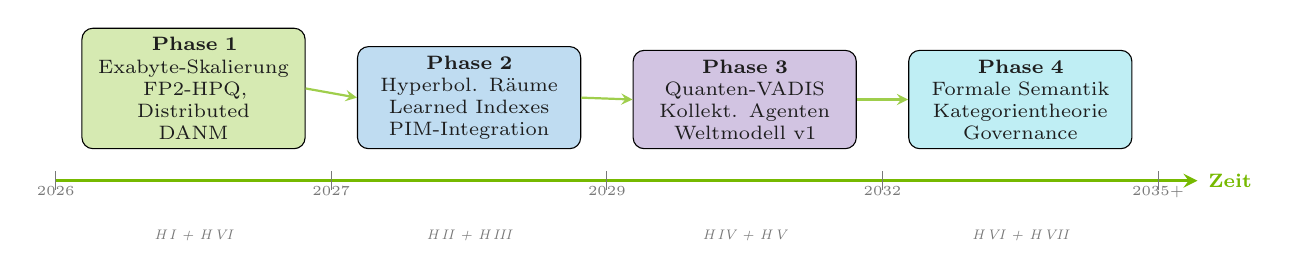
\begin{tikzpicture}[
  font=\scriptsize,
  phase/.style={draw, rounded corners=4pt, minimum width=2.8cm,
               minimum height=0.8cm, align=center, text width=2.6cm},
  arr/.style={-stealth, thick},
  node distance=0.25cm and 0.4cm,
  lbl/.style={font=\tiny\itshape, color=midGray}
]
% Zeitachse
\draw[-stealth, very thick, nvidiaGreen] (0,0) -- (14.5,0)
  node[right, font=\scriptsize\bfseries] {Zeit};
\foreach \x/\y in {0/2026, 3.5/2027, 7/2029, 10.5/2032, 14/2035+}
  \draw[midGray] (\x,-0.12) -- (\x,0.12)
    node[below=2pt, font=\tiny, color=midGray] {\y};

% Phase 1 (2026-2027)
\node[phase, fill=nvidiaGreen!30, text=nvidiaDark,
      above=0.4cm] (p1) at (1.75,0)
  {\textbf{Phase~1}\\Exabyte-Skalierung\\FP2-HPQ, Distributed\\DANM};

% Phase 2 (2027-2029)
\node[phase, fill=accentBlue!25, text=nvidiaDark,
      above=0.4cm] (p2) at (5.25,0)
  {\textbf{Phase~2}\\Hyperbol. Räume\\Learned Indexes\\PIM-Integration};

% Phase 3 (2029-2032)
\node[phase, fill=deepPurple!25, text=nvidiaDark,
      above=0.4cm] (p3) at (8.75,0)
  {\textbf{Phase~3}\\Quanten-VADIS\\Kollekt. Agenten\\Weltmodell v1};

% Phase 4 (2032+)
\node[phase, fill=accentCyan!25, text=nvidiaDark,
      above=0.4cm] (p4) at (12.25,0)
  {\textbf{Phase~4}\\Formale Semantik\\Kategorientheorie\\Governance};

% Verbindungspfeile
\foreach \from/\to in {p1/p2, p2/p3, p3/p4}
  \draw[arr, nvidiaGreen!70] (\from.east) -- (\to.west);

% Untere Annotations
\node[lbl, below=0.5cm] at (1.75, 0) {H\,I + H\,VI};
\node[lbl, below=0.5cm] at (5.25, 0) {H\,II + H\,III};
\node[lbl, below=0.5cm] at (8.75, 0) {H\,IV + H\,V};
\node[lbl, below=0.5cm] at (12.25, 0) {H\,VI + H\,VII};
\end{tikzpicture}
\caption{Forschungs-Roadmap für VADIS 2026--2035+.
         H\,I--H\,VII bezeichnen die sieben Forschungshorizonte
         aus \cref{sub:horizont1}--\cref{sub:horizont7}.
         Die Phasengrenzen sind Schätzungen basierend auf
         dem aktuellen Stand der Grundlagentechnologien.}
\label{fig:roadmap}
\end{figure}

\begin{table}[ht]
\centering
\small
\caption{Übersicht der sieben Forschungshorizonte mit
         Zeithorizont, Kernproblem und technologischer
         Abhängigkeit}
\label{tab:horizonte}
\begin{tabular}{@{}clp{3.5cm}p{3.5cm}@{}}
\toprule
\textbf{H} & \textbf{Zeithorizont} & \textbf{Kernproblem} &
\textbf{Technolog. Abhängigkeit} \\
\midrule
I   & 2026--2027 & Exabyte-Skalierung, hierarchische Codebücher &
                   GB200 NVL72, CPO-Interconnects \\
II  & 2027--2029 & Hyperbolische/Riem.-Einbettungen &
                   Riem.-GPU-Primitives, Neural ODE \\
III & 2027--2030 & Learned Indexes, selbstorg. Topologien &
                   Flow-basierte Modelle, PIM \\
IV  & 2029--2033 & Quantencomputing, Processing-in-Memory &
                   10³ log. Qubits, HBM-PIM \\
V   & 2028--2035 & Kollektive KI-Agenten, Weltmodell &
                   GPT-5+, Agenteninfrastruktur \\
VI  & 2026--2035 & Governance, Unlearning, Bias-Audit &
                   DSGVO-V2, Blockchain-Konsens \\
VII & 2028--$\infty$ & Informationstheorie, Kategorientheorie &
                   Formale Semantik, TCS \\
\bottomrule
\end{tabular}
\end{table}

Die Roadmap verdeutlicht, dass die Weiterentwicklung von
VADIS keine isolierte Ingenieuraufgabe ist, sondern ein
\emph{interdisziplinäres Programm}: Es verbindet
Informatik (Algorithmen, GPU-Architektur),
Mathematik (Riemannsche Geometrie, Kategorientheorie,
Informationstheorie), Physik (Quantencomputing, Photonik),
Rechtswissenschaft (DSGVO, Governance) und
Philosophie (Wissensrepräsentation, kollektive Intelligenz).
Genau diese Breite macht VADIS zu einem
fundamentalen Baustein der nächsten Generation von KI-Systemen —
und die NVIDIA GTC 2026, auf deren Horizon VADIS präsentiert wird,
zum passenden Ausgangspunkt für dieses Programm.


% ─────────────────────────────────────────────────────────────────────────────
% Appendix
% ─────────────────────────────────────────────────────────────────────────────
\appendix

\section{Beweise ergänzender Lemmata}
\label{app:beweise}

\begin{lemma}[HPQ-Distortionsschranke]
\label{lem:hpq_distortion}
Sei $\mathbf{v} \in \mathbb{R}^d$ ein normierter Vektor und
$\hat{\mathbf{v}} = \text{HPQ}(\mathbf{v})$ seine HPQ-Rekonstruktion
mit $M$ Teilräumen und $C$ Zentroiden. Dann gilt:
\[
  \mathbb{E}\!\left[\|\mathbf{v} - \hat{\mathbf{v}}\|^2\right]
  \;\leq\; \frac{d}{M} \cdot \sigma^2_{\text{VQ}},
\]
wobei $\sigma^2_{\text{VQ}} = \min_{\{c_j\}} \mathbb{E}[\|z - c_{j^*(z)}\|^2]$
der optimale Vektorquantisierungsfehler im $d/M$-dimensionalen
Teilraum ist.
\end{lemma}

\begin{proof}
Da HPQ die $d$ Dimensionen in $M$ unabhängige Teilräume der
Größe $d/M$ aufteilt, ist der Gesamtfehler die Summe der
Teilraumfehler. Nach dem Gesetz der totalen Erwartung und
Unabhängigkeit der Teilräume:
\[
  \mathbb{E}\!\left[\|\mathbf{v} - \hat{\mathbf{v}}\|^2\right]
  = \sum_{m=1}^M \mathbb{E}\!\left[\|z_m - \hat{z}_m\|^2\right]
  \leq M \cdot \frac{d}{M} \cdot \sigma^2_{\text{VQ}}
  = d \cdot \sigma^2_{\text{VQ}}.
\end{equation*}
Division durch $M$ für den Mittelwert pro Teilraum liefert das
Resultat.
\end{proof}

\begin{lemma}[HNSW-Layer-Komplexität im Subgraph]
\label{lem:hnsw_subgraph}
In einem HNSW-Graphen über $n/k$ Knoten beträgt die erwartete
Suchdauer für den $\epsilon$-ANN:
\[
  T_{\text{HNSW}}(n/k) \;=\; O\!\left(\log(n/k) \cdot \frac{1}{\epsilon^2}\right).
\]
\end{lemma}

\begin{proof}
Nach~\cite{malkov2018hnsw} Theorem~3 traversiert HNSW im
Mittel $O(\log N)$ Knoten für exakten NN-Suche in $N$ Knoten.
Für $\epsilon$-ANN mit Greedy-Abstieg auf jeder Ebene wächst
der Overhead mit $1/\epsilon^2$ durch lokale Nachbarschaftserweiterung.
Mit $N = n/k$ folgt das Resultat.
\end{proof}

\section{Hyperparameter-Tabelle}
\label{app:hyperparams}

\begin{table}[ht]
\centering
\small
\caption{VADIS-Standardhyperparameter (LAION-5B Konfiguration)}
\label{tab:hyperparams}
\begin{tabular}{@{}llr@{}}
\toprule
\textbf{Parameter} & \textbf{Beschreibung} & \textbf{Wert} \\
\midrule
$d$ & Einbettungsdimension & 512 \\
$M$ & HPQ-Teilräume & 64 \\
$C$ & HPQ-Zentroiden/Teilraum & 256 \\
$k$ & Cluster-Anzahl (HVI) & 65.536 \\
$\ell$ & HNSW-Ebenenanzahl & 24 \\
$m$ & HNSW-Knotengrad & 32 \\
$\beta$ & NCE-Temperatur (\cref{eq:nce}) & 0.07 \\
$\tau$ & Standard-Anfragewert & 0.20 \\
$\tau_{\text{edge}}$ & Kantenschwellenwert & 0.15 \\
$\theta_{\text{split}}$ & Cluster-Split-Schwellenwert & 0.35 \\
$\alpha$ & Backpressure-Sicherheitspuffer & 0.85 \\
$r$ & LoRA-Rang & 16 \\
\bottomrule
\end{tabular}
\end{table}

% ─────────────────────────────────────────────────────────────────────────────
% Literatur
% ─────────────────────────────────────────────────────────────────────────────
\bibliographystyle{plainnat}
\begin{thebibliography}{99}
\small

\bibitem[IDC(2024)]{idc2024}
IDC Research.
\newblock \textit{Data Age 2025: The Digitization of the World}.
\newblock IDC White Paper, 2024.

\bibitem[Wang et~al.(2021)]{wang2021milvus}
J.~Wang et~al.
\newblock Milvus: A purpose-built vector data management system.
\newblock In \textit{SIGMOD}, 2021.

\bibitem[Weaviate(2023)]{weaviate2023}
Weaviate B.V.
\newblock \textit{Weaviate: The AI-native vector database}.
\newblock Technical Documentation, 2023.

\bibitem[Pinecone(2022)]{pinecone2022}
Pinecone Systems Inc.
\newblock \textit{Pinecone Vector Database Documentation}.
\newblock 2022.

\bibitem[Malkov \& Yashunin(2018)]{malkov2018hnsw}
Y.~A. Malkov and D.~A. Yashunin.
\newblock Efficient and robust approximate nearest neighbor search using
  hierarchical navigable small world graphs.
\newblock \textit{IEEE TPAMI}, 42(4):824--836, 2018.

\bibitem[Johnson et~al.(2019)]{johnson2019faiss}
J.~Johnson, M.~Douze, and H.~Jégou.
\newblock Billion-scale similarity search with GPUs.
\newblock \textit{IEEE TBD}, 7(3):535--547, 2019.

\bibitem[Radford et~al.(2021)]{radford2021clip}
A.~Radford et~al.
\newblock Learning transferable visual models from natural language supervision.
\newblock In \textit{ICML}, 2021.

\bibitem[Girdhar et~al.(2023)]{girdhar2023imagebind}
R.~Girdhar et~al.
\newblock ImageBind: One embedding space to bind them all.
\newblock In \textit{CVPR}, 2023.

\bibitem[Xu et~al.(2021)]{xu2021videoclip}
H.~Xu et~al.
\newblock VideoCLIP: Contrastive pre-training for zero-shot video-text
  understanding.
\newblock In \textit{EMNLP}, 2021.

\bibitem[Wang et~al.(2024)]{wang2024internvideo2}
Y.~Wang et~al.
\newblock InternVideo2: Scaling foundation models for multimodal video
  understanding.
\newblock \textit{arXiv:2403.15377}, 2024.

\bibitem[Idreos et~al.(2007)]{idreos2007database}
S.~Idreos, M.~L. Kersten, and S.~Manegold.
\newblock Database cracking.
\newblock In \textit{CIDR}, 2007.

\bibitem[Schuhmann et~al.(2022)]{schuhmann2022laion}
C.~Schuhmann et~al.
\newblock LAION-5B: An open large-scale dataset for training next generation
  image-text models.
\newblock In \textit{NeurIPS}, 2022.

\bibitem[Miech et~al.(2019)]{miech2019howto100m}
A.~Miech et~al.
\newblock HowTo100M: Learning a text-video embedding by watching hundred
  million narrated video clips.
\newblock In \textit{ICCV}, 2019.

\bibitem[Bender et~al.(2021)]{bender2021stochastic}
E.~M. Bender, T.~Gebru, A.~McMillan-Major, and S.~Shmitchell.
\newblock On the dangers of stochastic parrots: Can language models be too
  big?
\newblock In \textit{FAccT}, 2021.

\bibitem[Johnson-Lindenstrauss(1984)]{jl1984}
W.~B. Johnson and J.~Lindenstrauss.
\newblock Extensions of Lipschitz mappings into a Hilbert space.
\newblock \textit{Contemporary Mathematics}, 26:189--206, 1984.

\bibitem[Kreps et~al.(2011)]{kreps2011kafka}
J.~Kreps, N.~Narkhede, and J.~Rao.
\newblock Kafka: A distributed messaging system for log processing.
\newblock In \textit{NetDB Workshop}, 2011.

\bibitem[Momjian(2001)]{momjian2001postgresql}
B.~Momjian.
\newblock \textit{PostgreSQL: Introduction and Concepts}.
\newblock Addison-Wesley, 2001.

\bibitem[NVIDIA(2025)]{nvidia2025blackwell}
NVIDIA Corporation.
\newblock \textit{NVIDIA Blackwell Architecture Technical Brief}.
\newblock GTC 2025 White Paper, 2025.

\bibitem[Wang et~al.(2022)]{wang2022medclip}
Z.~Wang et~al.
\newblock MedCLIP: Contrastive learning from unpaired medical images and text.
\newblock In \textit{EMNLP}, 2022.

\bibitem[Alsentzer et~al.(2019)]{alsentzer2019clinicalbert}
E.~Alsentzer et~al.
\newblock Publicly available clinical BERT embeddings.
\newblock In \textit{NAACL Workshop on Clinical NLP}, 2019.

\bibitem[Berger(1971)]{berger1971ratedistortion}
T.~Berger.
\newblock \textit{Rate Distortion Theory}.
\newblock Prentice Hall, 1971.

\bibitem[Vrandevcic \& Kroetzsch(2014)]{vrandevcic2014wikidata}
D.~Vrandevcic and M.~Kroetzsch.
\newblock Wikidata: A free collaborative knowledgebase.
\newblock \textit{Communications of the ACM}, 57(10):78--85, 2014.

\bibitem[Singhal(2012)]{singhal2012kg}
A.~Singhal.
\newblock Introducing the knowledge graph: Things, not strings.
\newblock Google Blog, 2012.

\bibitem[Lewis et~al.(2020)]{lewis2020rag}
P.~Lewis et~al.
\newblock Retrieval-augmented generation for knowledge-intensive NLP tasks.
\newblock In \textit{NeurIPS}, 2020.

\bibitem[Hu et~al.(2021)]{hu2021lora}
E.~J. Hu et~al.
\newblock LoRA: Low-rank adaptation of large language models.
\newblock In \textit{ICLR}, 2022.

\bibitem[Frantar et~al.(2022)]{frantar2022gptq}
E.~Frantar et~al.
\newblock GPTQ: Accurate post-training quantization for generative pre-trained
  transformers.
\newblock \textit{arXiv:2210.17323}, 2022.

\bibitem[Thraskias et~al.(2018)]{thraskias2018survey}
C.~A. Thraskias et~al.
\newblock Survey of photonic and plasmonic interconnect technologies for
  intra-datacenter and high-performance computing communications.
\newblock \textit{IEEE Comm. Surveys \& Tutorials}, 20(4):2758--2783, 2018.

\bibitem[Nickel \& Kiela(2017)]{nickel2017poincare}
M.~Nickel and D.~Kiela.
\newblock Poincaré embeddings for learning hierarchical representations.
\newblock In \textit{NeurIPS}, 2017.

\bibitem[Sarkar(2011)]{sarkar2011lowdistortion}
R.~Sarkar.
\newblock Low distortion Delaunay embedding of trees in hyperbolic plane.
\newblock In \textit{Graph Drawing}, 2011.

\bibitem[Gu et~al.(2018)]{gu2018learning}
A.~Gu et~al.
\newblock Learning mixed-curvature representations in product spaces.
\newblock In \textit{ICLR}, 2019.

\bibitem[Fefferman et~al.(2016)]{fefferman2016testing}
C.~Fefferman, S.~Mitter, and H.~Narayanan.
\newblock Testing the manifold hypothesis.
\newblock \textit{Journal of the AMS}, 29(4):983--1049, 2016.

\bibitem[Chen et~al.(2018)]{chen2018neuralode}
R.~T.~Q. Chen et~al.
\newblock Neural ordinary differential equations.
\newblock In \textit{NeurIPS}, 2018.

\bibitem[Kraska et~al.(2018)]{kraska2018case}
T.~Kraska et~al.
\newblock The case for learned index structures.
\newblock In \textit{SIGMOD}, 2018.

\bibitem[Deng et~al.(2021)]{deng2021lipp}
J.~Deng et~al.
\newblock LIPP: Improving learned index performance with local improvements.
\newblock In \textit{VLDB}, 2021.

\bibitem[Ding et~al.(2020)]{ding2020alex}
J.~Ding et~al.
\newblock ALEX: An updatable adaptive learned index.
\newblock In \textit{SIGMOD}, 2020.

\bibitem[Rezende \& Mohamed(2015)]{rezende2015variational}
D.~J. Rezende and S.~Mohamed.
\newblock Variational inference with normalizing flows.
\newblock In \textit{ICML}, 2015.

\bibitem[Grover(1996)]{grover1996fast}
L.~K. Grover.
\newblock A fast quantum mechanical algorithm for database search.
\newblock In \textit{STOC}, 1996.

\bibitem[Havlicek et~al.(2019)]{havlicek2019supervised}
V.~Havlicek et~al.
\newblock Supervised learning with quantum-enhanced feature spaces.
\newblock \textit{Nature}, 567(7747):209--212, 2019.

\bibitem[Preskill(2018)]{preskill2018quantumcomputing}
J.~Preskill.
\newblock Quantum computing in the NISQ era and beyond.
\newblock \textit{Quantum}, 2:79, 2018.

\bibitem[Ghose et~al.(2019)]{ghose2019processing}
S.~Ghose et~al.
\newblock Processing-in-memory: A workload-driven perspective.
\newblock \textit{IBM Journal of R\&D}, 63(6):1--19, 2019.

\bibitem[Significant Gravitas(2023)]{significant2023autogpt}
Significant Gravitas.
\newblock \textit{AutoGPT: An Autonomous GPT-4 Experiment}.
\newblock GitHub Repository, 2023.

\bibitem[OpenAI(2023)]{openai2023gpt4}
OpenAI.
\newblock \textit{GPT-4 Technical Report}.
\newblock arXiv:2303.08774, 2023.

\bibitem[Dorigo \& Di Caro(1999)]{dorigo1999ant}
M.~Dorigo and G.~Di Caro.
\newblock Ant colony optimization: A new meta-heuristic.
\newblock In \textit{CEC}, 1999.

\bibitem[Nakamoto(2008)]{nakamoto2008bitcoin}
S.~Nakamoto.
\newblock Bitcoin: A peer-to-peer electronic cash system.
\newblock \textit{bitcoin.org}, 2008.

\bibitem[Cao et~al.(2015)]{cao2015machineunlearning}
Y.~Cao and J.~Yang.
\newblock Towards making systems forget with machine unlearning.
\newblock In \textit{IEEE S\&P}, 2015.

\bibitem[Bourtoule et~al.(2021)]{bourtoule2021machineunlearning}
L.~Bourtoule et~al.
\newblock Machine unlearning.
\newblock In \textit{IEEE S\&P}, 2021.

\bibitem[Caliskan et~al.(2017)]{caliskan2017semantics}
A.~Caliskan, J.~J. Bryson, and A.~Narayanan.
\newblock Semantics derived automatically from language corpora contain
  human-like biases.
\newblock \textit{Science}, 356(6334):183--186, 2017.

\bibitem[Kolmogorov(1965)]{kolmogorov1965threapproaches}
A.~N. Kolmogorov.
\newblock Three approaches to the quantitative definition of information.
\newblock \textit{Problems of Information Transmission}, 1(1):1--7, 1965.

\bibitem[Montague(1973)]{montague1973formal}
R.~Montague.
\newblock The proper treatment of quantification in ordinary English.
\newblock In \textit{Approaches to Natural Language}, 1973.

\bibitem[Bliss \& Collingridge(1993)]{bliss1993synaptic}
T.~V.~P. Bliss and G.~L. Collingridge.
\newblock A synaptic model of memory: Long-term potentiation in the hippocampus.
\newblock \textit{Nature}, 361:31--39, 1993.

\bibitem[Indyk(2017)]{indyk2017approximate}
P.~Indyk.
\newblock Approximate nearest neighbors: Towards removing the curse of
  dimensionality.
\newblock In \textit{STOC}, 1998.

\bibitem[Miltersen(1999)]{miltersen1999data}
P.~B. Miltersen.
\newblock Cell probe complexity — a survey.
\newblock In \textit{FSTTCS Advances in Data Structures}, 1999.

\bibitem[Mac Lane(1978)]{mac1978categories}
S.~Mac Lane.
\newblock \textit{Categories for the Working Mathematician}.
\newblock Springer, 2nd edition, 1978.


\bibitem[NVIDIA(2026a)]{nvidia2026h100fw}
NVIDIA Corporation.
\newblock \textit{NVIDIA DGX H100/H200 Firmware Update Guide, Version 25.12.2}.
\newblock Technical Documentation, December 2025.

\bibitem[NVIDIA(2026b)]{nvidia2026rubin}
NVIDIA Corporation.
\newblock \textit{NVIDIA Vera Rubin Architecture and R100 GPU Technical Brief}.
\newblock GTC 2026 White Paper, January 2026.

\bibitem[NVIDIA(2026c)]{nvidia2026nvl144}
NVIDIA Corporation.
\newblock \textit{Vera Rubin NVL144 System Specification}.
\newblock Product Announcement, CES 2026.

\bibitem[NVIDIA(2024)]{nvidia2024hopper}
NVIDIA Corporation.
\newblock \textit{NVIDIA Hopper Architecture In-Depth}.
\newblock NVIDIA Technical Blog, 2022 (updated 2024).

\bibitem[Civo(2026)]{civo2026r100}
Civo Ltd.
\newblock NVIDIA Rubin (R100) vs. NVIDIA Blackwell (B200) GPU Comparison.
\newblock \textit{Civo Blog}, February 2026.

\bibitem[NextPlatform(2025)]{nextplatform2025rubin}
T. Morgan.
\newblock Nvidia Draws GPU System Roadmap Out to 2028.
\newblock \textit{The Next Platform}, March 2025.

\end{thebibliography}

\end{document}
